%%% use 10pt options with the asme2ej format
\documentclass[10pt]{asme2ej}

\usepackage{graphicx,epsfig,color,textcomp,amssymb,amsmath,mathrsfs,cancel,bbm,ulem}

%% The class has several options
%  onecolumn/twocolumn - format for one or two columns per page
%  10pt/11pt/12pt - use 10, 11, or 12 point font
%  oneside/twoside - format for oneside/twosided printing
%  final/draft - format for final/draft copy
%  cleanfoot - take out copyright info in footer leave page number
%  cleanhead - take out the conference banner on the title page
%  titlepage/notitlepage - put in titlepage or leave out titlepage
%  
%% The default is oneside, onecolumn, 10pt, final


\title{Mechanical Modeling of a Neuron Embedded in Collagenous Tissue}

%%% first author
\author{Victor W. L. Chan
    \affiliation{
	Scientific Computation Research Center,\\
	Rensselaer Polytechnic Institute,\\
	Low Center for Industrial Innovation, CII-4011,\\
	110 8th Street,\\
	Troy, NY 12180
    }	
}

%%% second author
%%% remove the following entry for single author papers
%%% add more entries for additional authors
\author{William R. Tobin 
    \affiliation{ Scientific Computation Research Center,\\
	Rensselaer Polytechnic Institute,\\
	Low Center for Industrial Innovation, CII-4011,\\
	110 8th Street,\\
	Troy, NY 12180
    }
}

%%% third author
%%% remove the following entry for single author papers
%%% add more entries for additional authors
\author{Sijia Zhang
    \affiliation{ Department of Bioengineering,\\
        University of Pennsylvania,\\
	240 Skirkanich Hall,\\
        210 South 33rd Street,\\
         Philadelphia, PA 19104
    }
}

\author{Beth A. Winkelstein
    \affiliation{ Department of Bioengineering,\\
        University of Pennsylvania,\\
	240 Skirkanich Hall,\\
        210 South 33rd Street,\\
         Philadelphia, PA 19104
    }
}

\author{Victor H. Barocas
    \affiliation{ Department of Biomedical Engineering,\\
        University of Minnesota,\\
	7-105 Nils Hasselmo Hall,\\
        312 Church Street SE,\\
        Minneapolis, MN 55455
    }
}

\author{Mark S. Shephard
    \affiliation{ Scientific Computation Research Center,\\
	Rensselaer Polytechnic Institute,\\
	Low Center for Industrial Innovation, CII-4011,\\
	110 8th Street,\\
	Troy, NY 12180
    }
}

\author{Catalin R. Picu
       \thanks{Address all correspondence for other issues to this author.} 
        \affiliation{ Scientific Computation Research Center,\\
	Rensselaer Polytechnic Institute,\\
	Low Center for Industrial Innovation, CII-4011,\\
	110 8th Street,\\
	Troy, NY 12180\\
	email: picuc@rpi.edu
    }
}



\begin{document}

\maketitle    

%%%%%%%%%%%%%%%%%%%%%%%%%%%%%%%%%%%%%%%%%%%%%%%%%%%%%%%%%%%%%%%%%%%%%%
\begin{abstract}
{\it 
Needs to be filled in.
}
\end{abstract}

%%%%%%%%%%%%%%%%%%%%%%%%%%%%%%%%%%%%%%%%%%%%%%%%%%%%%%%%%%%%%%%%%%%%%%
\section{Introduction}

Excessive loading in facet capsule ligament (FCL) induces damage to collagen network and axons of innervating neurons [references].``Although injurious ligament loading is known to activate nociceptors for pain signaling, the local biomechanical mechanisms by which neurons are injured, their biomechanical vulnerability, and the resulting physiological dysfnction are still poorly understood \cite{Zhang:2016ga}.'' Recently, an integrated experimental and modeling approach was employed to examine the responses of neurons and the surrounding collagen fibers to ligamentous matrix loading. This approach provided initial understanding of how macroscopic deformation is translated to neuronal loading and signaling \cite{Zhang:2016ga}. In this paper, we build on the work of Zhang et al. \cite{Zhang:2016ga} and examine the mechanical interaction between neuron and surrounding collagen gel.  In order to capture the fibrillar microstructure of the collagen gel surrounding the neuron, we use a volume-averaged multi-scale model \cite{Chandran:2007hy,Stylianopoulos:2007dp}. The multi-scale model has been previously used to model the passive mechanical contribution of cells in collagen gel, where the cell was represented with a simple spherical geometry \cite{Lai:2013fp}. In this paper, we expand on the previous work by considering a realistic geometry of the neuron, which is reconstructed from images taken experimentally. The multi-scale model is implemented in the adaptive multi-scale simulation infrastructure (AMSI) [reference for AMSI?].

%%%%%%%%%%%%%%%%%%%%%%%%%%%%%%%%%%%%%%%%%%%%%%%%%%%%%%%%%%%%%%%%%%%%%%
\section{Materials and Methods}
To investigate the mechanical interaction between neuron and surrounding collagen gel, a geometric model and its corresponding finite-element mesh is generated from confocal images of an individual neuron from a neuronal culture that was developed to mimic innervation of collagenous tissue (see Ref.\ \citenum{Zhang:2016ga} for preparation of neuronal culture). Thereby, the complex geometry of the neuron is incorporated into our simulations and enables us to extend our findings to realistic physiological environments. In this section, the details for modeling a neuron that is embedded in a collagen gel is provided. 

%=========================================================================================================
\subsection{Generation of Model and Finite-Element Mesh from Experimental Images}
Confocal images were taken from a neuronal culture that was developed to mimic innervation of collagenous tissue. Briefly, dissociated dorsal root ganglion neurons were embedded in three-dimensional collagen I gels. Immunocytochemistry was performed with an antibody against the cytoskeletal protein $\beta$III-tubulin (Abcam Cambridge, MA) to label for neuronal structure. Z-stack Images (2-micron thick) were taken by a Zeiss LSM 510 confocal microscope (Carl Zeiss Inc., Thornwood, NY) using a 40X objective and with a resolution of 0.22 micron/pixel. The segmented stack of confocal images are shown schematically in Fig.\ \ref{fig:image_to_model}(a). The confocal images are converted to a geometric model using Simmetrix's \textit{ImageToModel} tool \cite{Klaas_chapter, Klaas_conference, simmetrix} and its corresponding mesh was generated using Simmetrix meshing tools \cite{simmetrix,Shephard:2000vc}. The neuron-in-gel model and its corresponding mesh is shown in Figs.\ \ref{fig:image_to_model}(b) and (c), respectively. 
%
% (a) Schematic of image stack - images from N2P30/Neuron/sample2 folder. 
% (b) Neuron-in-gel model. Image generated by simModeler.
% (c) Neuron-in-gel mesh. Image generated by Paraview. N2P178/3-Neuron_FT
\begin{figure}[ht]
\begin{center}
$
\begin{array}{ccc}
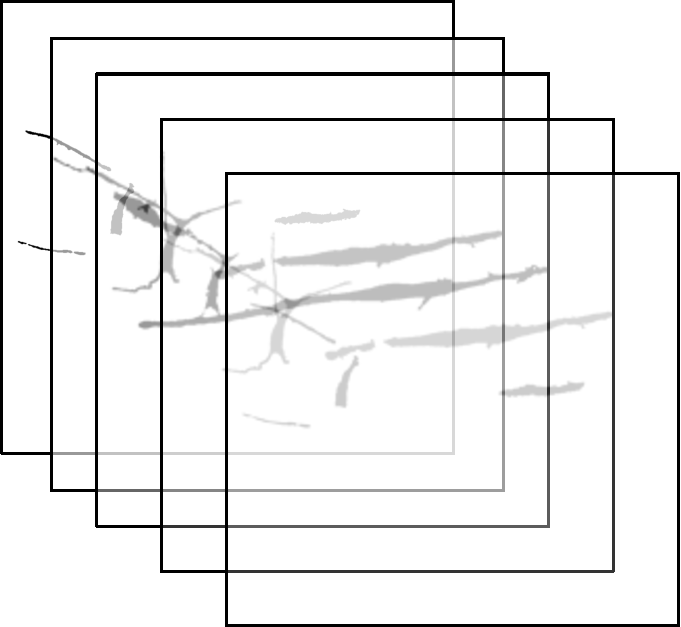
\includegraphics[height=3.5cm]{figure/ImageStack.pdf} & 
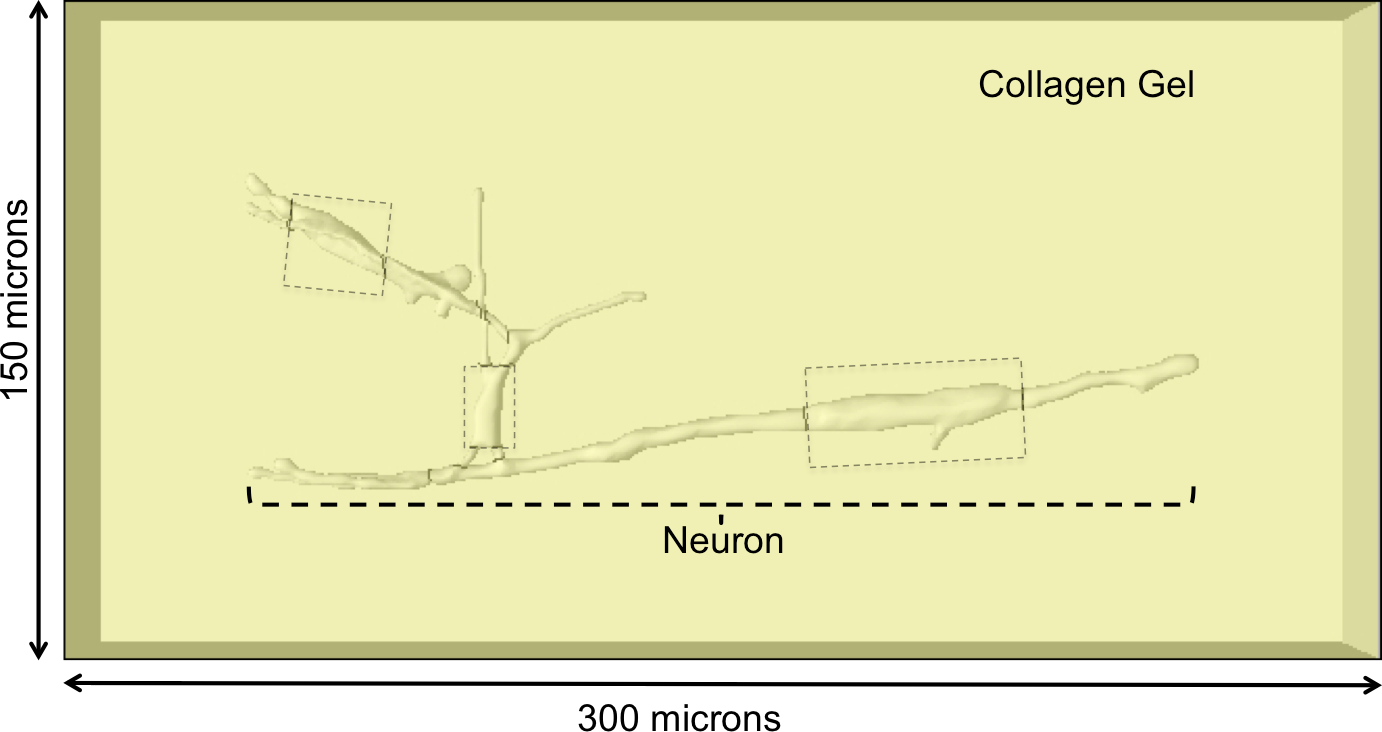
\includegraphics[height=3.5cm]{figure/neuron-in-gel_labels.pdf} &
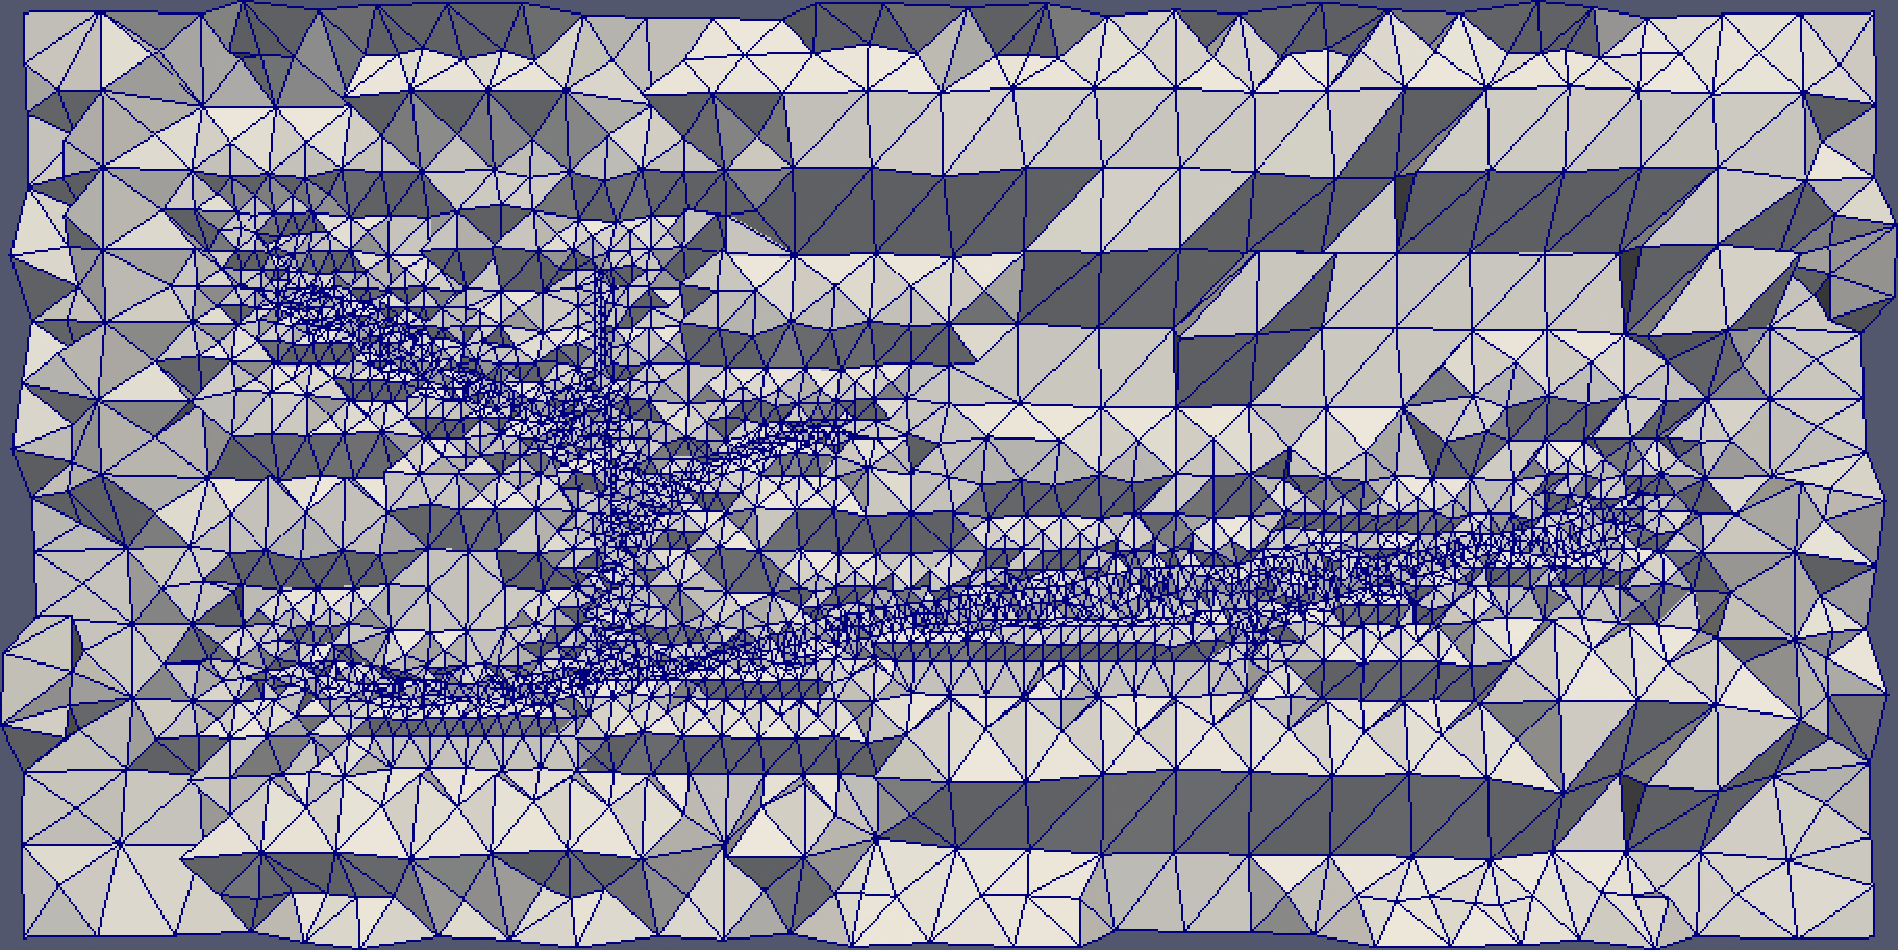
\includegraphics[height=3.5cm]{figure/neuron-in-gel_mesh.pdf} \\
(a) & (b) & (c)
\end{array}
$
\end{center}
\caption{\label{fig:image_to_model} (a) Stack of confocal images of a neuron from neuronal culture. (b) Model of neuron embedded in collagen gel that is generated from Simmetrix's \textit{ImageToModel} tool \cite{Klaas_chapter, Klaas_conference, simmetrix}. Regions in the neuron that are marked with dashed rectangles are the cell bodies, while those that are not marked constitute the axons of the neuron. The region enclosing the neuron is the collagen gel. (c) Cut in neuron-in-gel model showing the mesh generated from Simmetrix meshing tools \cite{simmetrix,Shephard:2000vc}. A mesh of ~80k tetrahedral elements is used for simulations in this work.}
\end{figure}
%

%=========================================================================================================
\subsection{Multi-Scale Modeling of Collagen Gel}
Soft biological tissue consisting of collagen I has been adequately modeled using a multi-scale formulation based on volume-averaging \cite{Chandran:2007hy,Stylianopoulos:2007dp,Barocas:2007gk,Lai:2012ji,Lake:2012jm}. The multi-scale formulation consists of two scales: the microscopic scale that represents the fiber level and the macroscopic scale that represents the tissue level. The mathematical formulation for the volume-averaged multi-scale method is summarized here. For a detailed formulation, see Refs.\ \citenum{Chandran:2007hy,Stylianopoulos:2007dp}. The choice of input parameters for the multi-scale model, which are based on experimental values, is then described. 

%----------------------------------------------------------------------------------------------------------------------------------------------------------------------------------------
\subsubsection{Mathematical Formulation}
The microscopic scale is represented by a collagen network that defines the representative volume element (RVE). In our model, each RVE is generated from a Delaunay triangulation of randomly placed seed points - the edges of the triangulation represent the fibers of the network. Fiber networks with network density (total length of fibers/total number of fibers) of 100 ($\pm$ 1) were used in our simulations where the force on each fiber is
%
\begin{equation}
T_i^{(m)} = \frac{E_f A_f}{B} \left[ \exp(B\varepsilon_f^{(m)}) - 1\right],
\label{eq:fiber_force}
\end{equation}
%
where $E_f$ is the linear modulus of the collagen fiber, $A_f$ is the fiber cross-sectional area, $B$ is a constant, and $\varepsilon_f \equiv 0.5(\lambda_f - 1)$ is the fiber's Green strain, where $\lambda_f$ is the fiber stretch ratio.  The superscripts $(m)$ indicate values of the microscopic scale. The boundary deformations for each RVE is determined by the macroscopic deformation state of the macroscopic scale (down-scaling).

Upon solving for fiber-force equilibrium at each RVE, the microscopic scale is coupled to the macroscopic scale via volume averaging, where the elements of the macroscopic Cauchy stress tensor can be calculated from the equilibrium microscopic fiber forces by (up-scaling)\cite{Chandran:2007hy,Stylianopoulos:2007dp}
%
\begin{equation}
\sigma_{ij}^{(M)} = \frac{1}{V^{(m)}} \sum_{n \in bcl} {}^n x_i^{(m)} {}^n T_j^{(m)}.
\label{eq:macro_stress_discrete}
\end{equation}
%
In Eq.\ \eqref{eq:macro_stress_divergence}, ${}^nx_i^{(m)}$ is the $i^{th}$ coordinate of the $n^{th}$ cross-link on the boundary of the RVE ($bcl$) and ${}^nT_j^{(m)}$ is the $j^{th}$ component of the internal force of the $n^{th}$ cross-link on the boundary. The superscripts $(M)$ indicate values of the macroscopic scale. The Cauchy stress tensor obtained from the microscopic scale are used to solve the macroscopic force balance \cite{Chandran:2007hy,Stylianopoulos:2007dp}
%
\begin{equation}
\sigma_{ij,i}^{(M)} = \frac{1}{V^{(m)}} \int_{\partial V^{(m)}} \left( s_{ij}^{(m)} - \sigma_{ij}^{(M)} \right)u_{k,i}^{(m)} n_k dA^{(m)},
\label{eq:macro_stress_divergence}
\end{equation}
%
where $u_k^{(m)}$ is the displacement of the RVE boundary on the microscale, $n_k$ is the unit normal vector, and $s_{ij}^{(m)}$ are elements of the microscopic stress tensor. The right-hand side of Eq.\ \eqref{eq:macro_stress_divergence} accounts for the correlation between the inhomogeneous displacement of the RVE boundary and local inhomogeneities in the stress field. 

%----------------------------------------------------------------------------------------------------------------------------------------------------------------------------------------
\subsubsection{Parameterization of fiber network}
The RVEs used in the multi-scale simulations are generated in a unit-cube compute domain that ranges from -0.5 to 0.5. In order to couple the Cauchy stress from microscopic to the macroscopic scale, the compute RVE must be properly scaled to the physical domain. In this study, the scaling between the compute and physical domains is determined by comparing the average fiber length in the RVEs to that in reconstituted collagen type I networks \cite{Lindstrom:2013gd} with collagen concentration of 2g/L. The average fiber length in the RVEs is 0.26 while that in the reconstituted collagen type I network is 1.81 $\mu$m \cite{Lindstrom:2013gd}. Based on these average lengths, a unit length in the compute  domain (average length is 0.26) is equivalent to 7 $\mu$m in the physical domain (average length is 1.81 $\mu$m); the scaling of $L=7 \ \mu$m is determined from the ratio 1.81 $\mu m$ / 0.26. Along the same line of argument, the Cauchy stresses calculated in the compute domain are scaled by $1/L^2$ to obtain Cauchy stresses for the physical domain.

To solve the microscopic scale fiber-force problem, the parameters in Eq.\ \eqref{eq:fiber_force} must be specified. The value of $A_f$ is set according to Ref.\ \citenum{Dutov:2016gu} where the fiber radius of rat tail collagen I was measured to be 162 $\mu$m. The values for $E_f$ and $B$ are set by fitting to experimentally measured stress-strain curves of rat tail collagen I gels (see Ref.\ \citenum{Zhang:2016ga} for preparation of collagen samples). To obtain the stress-strain responses experimentally, collagen I gels underwent uniaxial tensile loading at 0.5m/s to 8mm using an Instron 5865 (Instron, Norwood, MA), as described in Ref.\ \citenum{Zhang:2016ga}. The Instron Bluehill software collected the force and displacement data at 1kHz during loading. \textcolor{red}{[ Need to describe how force-displacement data is converted to stress-strain data.]} The stress-strain curves calculated from simulation and measured experimentally are shown in Fig.\ \ref{fig:fiber_param}(a), where $E_f = 200$ kPa and $B=20$ for the RVEs used in the simulation. 
%
% (a) stress-strain curve from N2P178/1-NewParams_Cube/stress-strain folder.
% (b) fiber force curve from N2P177/LRT_Compression folder.
\begin{figure}[ht]
\begin{center}
$
\begin{array}{cc}
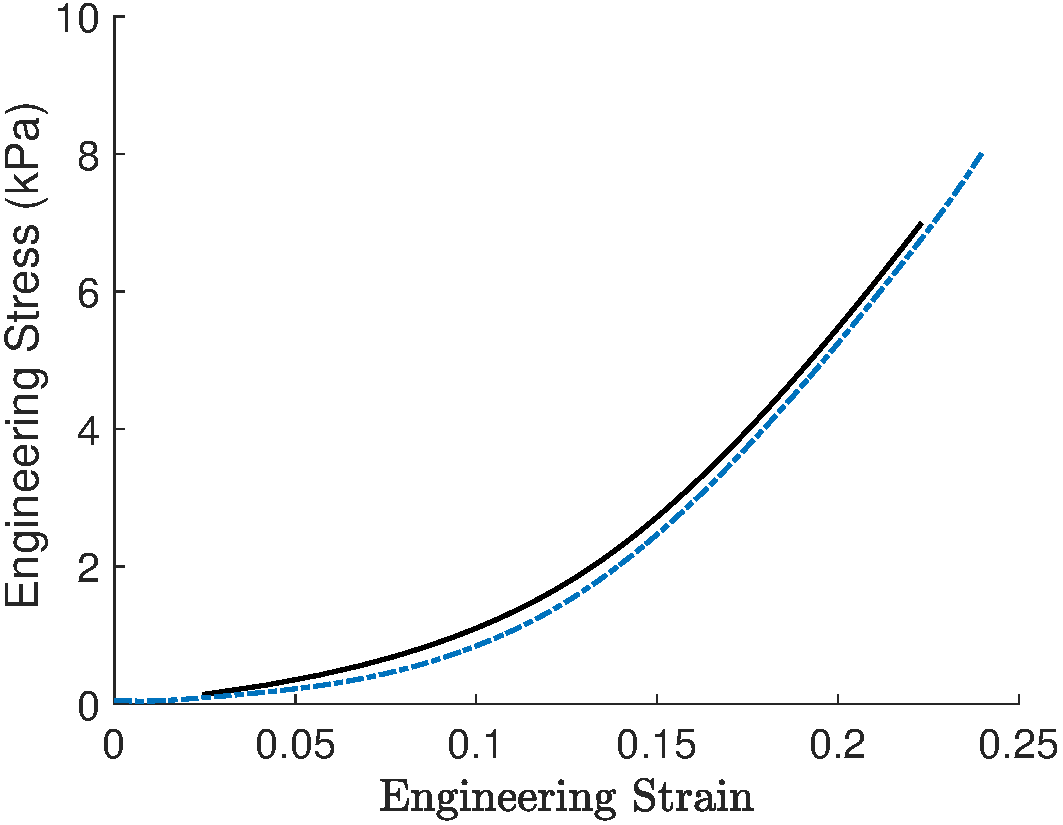
\includegraphics[height=5cm]{figure/stress_strain.pdf} &
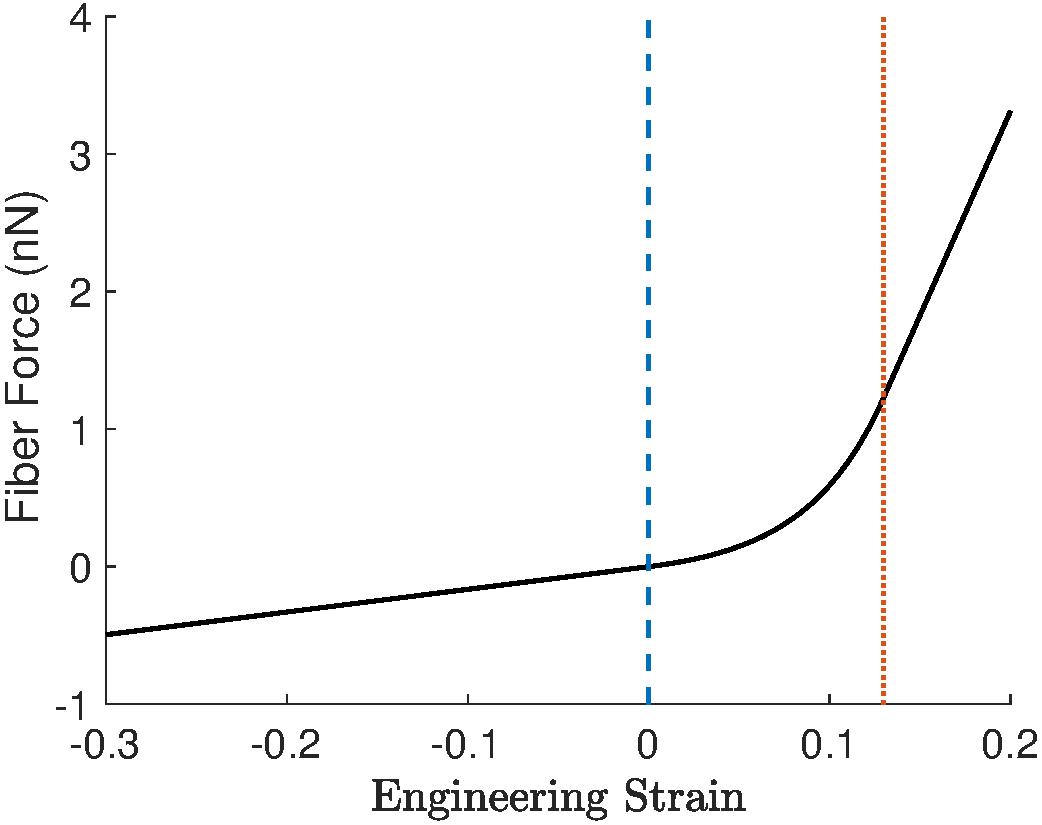
\includegraphics[height=5cm]{figure/FiberForceRelation.pdf} \\ 
(a) & (b) 
\end{array}
$
\end{center}
\caption{\label{fig:fiber_param} Plots of (a) stress-strain curve calculated from simulation (blue ``x'') and measured experimentally (black line),  and (b) fiber-force relationship for RVEs used in the simulation (blue ``x") and from Eq.\ \eqref{eq:fiber_force} (black line). The parameters of the fiber-force relationship (Eq.\ \eqref{eq:fiber_force}) are $E_f = 200$ kPa and $B=20$. The fiber force used in the simulation transitions to a linear fiber force at 13$\%$ fiber stretch - the stiffness in tension beyond 13$\%$ fiber stretch ($E_T$) is 29.7 kPa. The stiffness in compression ($E_C$) is set to the slope of Eq.\ \eqref{eq:fiber_force} at zero fiber stretch, which is 1.65 kPa.}
\end{figure}
%

In order to achieve the stress-strain fit shown in Fig.\ \ref{fig:fiber_param}(a), the exponential fiber force of Eq.\ \eqref{eq:fiber_force} is made to transition to a linear fiber-force relationship at a fiber stretch ratio of $13\%$ in tension;  the tensile stiffness for each fiber in the RVE stays constant at 29.7 kPa for fiber stretch ratios above $13\%$. Additionally, the fiber stiffness in compression is set the slope of Eq.\ \eqref{eq:fiber_force} at zero fiber stretch, which is 1.65 kPa in order to prevent the RVE fiber network from collapsing at large deformations; the fiber force from Eq.\ \eqref{eq:fiber_force} and that used in the simulations are shown in Fig.\ \ref{fig:fiber_param}(b).

The Poisson ratio is measured from the volume change of the domain via
%
\begin{equation}
\nu = \frac{1}{2}\left(1- \frac{\Delta V}{V_0}\frac{l_0}{\Delta l}\right).
\label{eq:poisson-ratio}
\end{equation}
%
The Poisson ratio as a function of applied bulk strain for the fiber-force relationship used to calculate the stress-strain curve in Fig.\ \ref{fig:fiber_param}(a) is plotted in Fig.\ \ref{fig:fiber_param2}(a). The Poisson ratio increases as a function of applied strain, and becomes larger than 0.5 at an applied strain of approximately $15\%$. The behavior of increasing Poisson ratio is consistent with experiments \cite{Vader:2009js}, however the values of Poisson ratio measured experimentally is significantly larger than what is seen in our simulations. \textcolor{red}{This difference in the Poisson ratio can be attributed to the inability of our continuum model to represent the mechanisms that arise in actual collagen fiber networks.}
%
% (a) Poisson ratio curve from N2P178/1-NewParams_Cube/poisson-ratio folder.
% (b) Alignment curve from N2P178/1-NewParams_Cube/alignment folder.
\begin{figure}[ht]
\begin{center}
$
\begin{array}{cc}
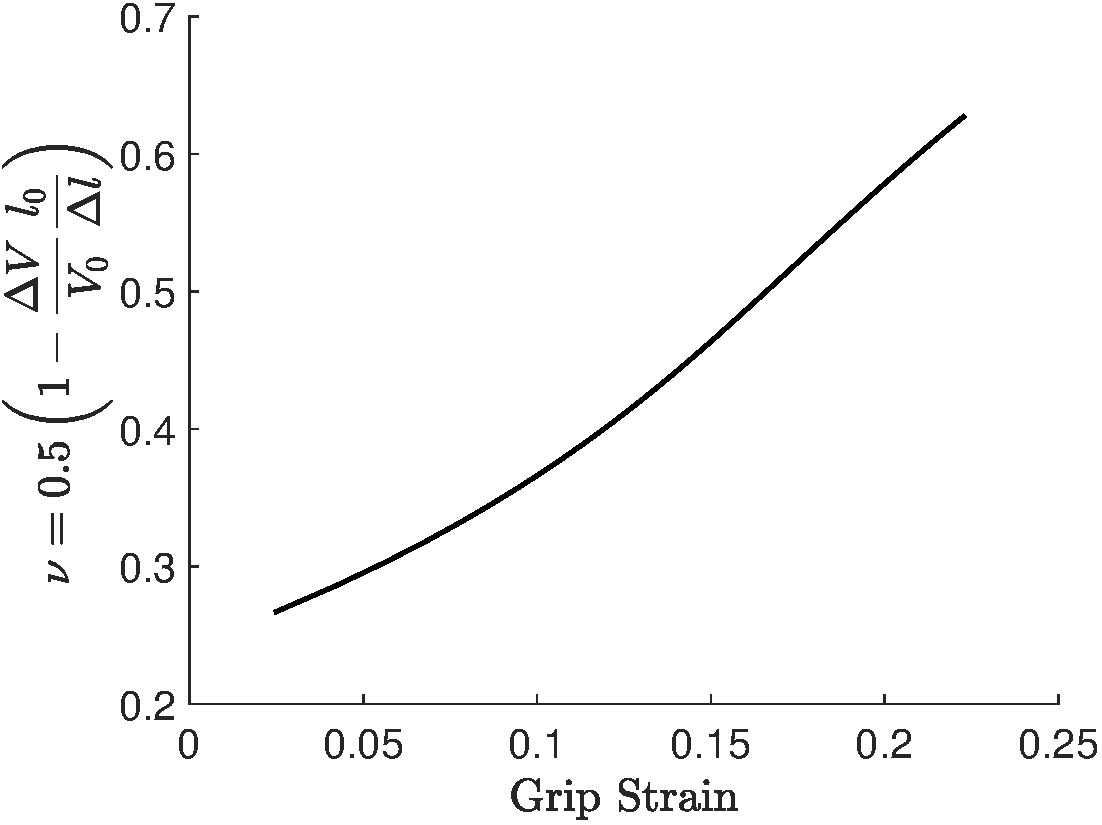
\includegraphics[height=5cm]{figure/PoissonRatio.pdf} &
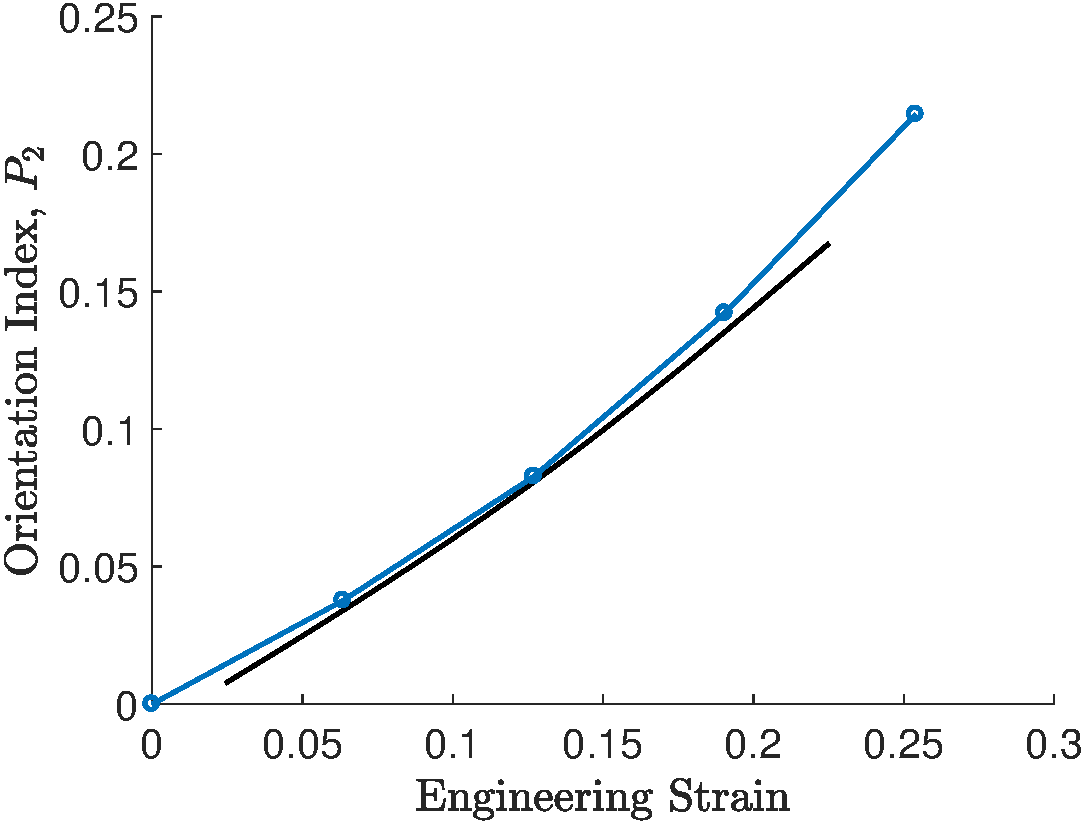
\includegraphics[height=5cm]{figure/alignment.pdf} \\ 
(a) & (b)
\end{array}
$
\end{center}
\caption{\label{fig:fiber_param2} Plots of (a) Poisson ratio calculated from simulation and (b) fiber alignment metric $P_2$ calculated from simulation (blue ``x") and measured experimentally (black line). Simulation results are calculated with fiber-force relationship used to obtain stress-strain curve in Fig.\ \ref{fig:fiber_param}.}
\end{figure}
%

The fiber alignment in innervated collagenous tissue was measured using the QPLI method \cite{Quinn:2009bf} where alignment angle $\alpha$ and retardation $\delta$ is measured in each pixel. Our customized QPLI system is comprised of a fiber-optic light source (Dolan-Jenner Industries Inc., Boxborough, MA), a motor-controlled linear polarizer (Edmund Optics, Barrington, NJ) that rotates at 750 rpm, and a circular analyzer mounted to a high-speed camera (Phantom-v9.1; Vision Research Inc, Wayne, NJ) \textcolor{red}{(Ref. 1)}. The QPLI system was integrated with the mechanical testing device, and collagen I gels were placed between the rotating polarizer and the circular analyzer. Polarized light images were acquired during tensile loading at 500 fps with 14.5 pixel/mm resolution and processed using harmonic analysis to extract the alignment angle and retardation (\textcolor{red}{ref: Tower, Neidert and Tranquillo 2002; Quinn and Winkelstein, 2008}).  To compare fiber alignment that is measured experimentally and calculated from simulations, the orientation index $P_2$ is considered. The value of $P_2$ is calculated from the angle $\theta$ between fibers and the direction of alignment
%
\begin{equation}
P_2 = \frac{3 <\cos^2\theta> - 1}{2},
\label{eq:P2_simulation}
\end{equation}
%
where $<a>$ denotes the average of $a$. The value of $P_2$ ranges from 1 ($\theta=0$ or $\pi$) in which the fibers are completely aligned to -1/2 ($\theta=\pi/2$) in which the fibers are orthogonal to the alignment direction. When $P_2=0$, the fiber network is randomly oriented. The orientation index $P_2$ can be calculated from $\alpha$ and $\delta$ of the QPLI method via
%
\begin{align}
&P_2 = \int_0^{\pi} p(\theta) \cos^2\theta d\theta \nonumber\\
&p(\theta) = \frac{1}{N} \sum_{i=1}^N \left[ \frac{1-2\delta_i}{\pi} + \frac{4 \delta_i}{\pi}\cos^2(\theta - \alpha_i)\right],
\label{eq:P2_experiment}
\end{align}
%
where $\delta_i$ and $\alpha_i$ are the retardation and alignment angle, respectively, of the $i^{th}$ pixel. The fiber alignment as a function of bulk applied strain calculated from simulation and measured experimentally is plotted in Fig.\ \ref{fig:fiber_param2}(b). As expected, the fibers become more aligned as applied strain increases - the alignment in the RVE is stronger than in experiment for the same amount applied strain. \textcolor{red}{[The stronger alignment in the RVE is likely due to the large coordination of Delaunay network used in our model.]}

%=========================================================================================================
\subsection{Constitutive Relationship to Model Neuron}
Cross-linked microtubule bundles that are axially aligned are a major structural feature of axons, giving rise to anisotropic mechanical behavior \cite{Peter:2012fc}. To account for such mechanical anisotropy, the axons are modeled as a transversely isotropic hyperelastic material \cite{JavierBonet:2008uxa,Bonet:1998vc}. The alignment of the microtubule bundles decrease within the cell bodies causing the mechanical behavior to become more isotropic \textcolor{red}{[Need to find references that supports this]}. To capture such behavior, the cell bodies are modeled as a transversely isotropic hyperelastic material where the axial stiffness is a function of distance from the cell-body/axon interface - the axial stiffness is lowest at the center of the cell body. 

%----------------------------------------------------------------------------------------------------------------------------------------------------------------------------------------
\subsubsection{Mathematical Formulation}
A compressible transversely isotropic neo-Hookean model is used to model \cite{Bonet:1998vc} the axons and cell bodies of the neuron. The elements of the Cauchy stress tensor and spatial elasticity tensor can be expressed in terms of neo-Hookean (nh) and transversely isotropic (trns) components \cite{Bonet:1998vc}
%
\begin{equation}
\sigma_{ij} = \sigma^{\text{nh}}_{ij} + \sigma^{\text{trns}}_{ij} \ \ \text{ and } \ \ c_{ijkl} = c^{\text{nh}}_{ijkl} + c^{\text{trns}}_{ijkl},
\end{equation}
%
respectively, where 
%
\begin{align}
&\sigma^{\text{nh}}_{ij} = \frac{\mu}{J}(b_{ij} - \delta_{ij}) + \lambda(J-1)\delta_{ij} \nonumber\\
%
&\sigma^{\text{trns}}_{ij} = \frac{2\beta}{J}(a_r a_r - 1)\delta_{ij} + \frac{2}{J}[\alpha+2\beta\ln J+2\gamma(a_r a_r -1)]a_i a_j - \frac{\alpha}{J}(b_{is}a_s a_j+a_i b_{jr}a_r) \nonumber\\
%
&c^{\text{nh}}_{ijkl} = \lambda(2J-1)\delta_{ij}\delta_{kl} + \frac{2}{J}[\mu - \lambda J(2J-1)]\delta_{ik}\delta_{jl} \nonumber\\
%
&c^{\text{trns}}_{ijkl} = \frac{8\gamma}{J}a_i a_j a_k a_l + \frac{4\beta}{J}(a_i a_j \delta_{kl} + \delta_{ij}a_k a_l) - \frac{\alpha}{J}(a_i a_l b_{jk} + b_{ik}a_j a_l) - \frac{4\beta}{J}(a_r a_r - 1)\delta_{ik}\delta_{jl}.
\label{eq:trns_iso}
\end{align}
%
The constants of Eq.\ \eqref{eq:trns_iso} are defined as
%
\begin{align}
&\lambda = \frac{2\mu (\nu+n\nu^2)}{m} \ \ \ \ \ \gamma = \frac{E_A(1-\nu)}{8m} - \frac{\lambda+2\mu}{8} + \frac{\alpha}{2} - \beta \nonumber\\
%
&\alpha = \mu - G_A \ \ \ \ \ \ \ \ \ \ \ \ \ \ m = 1 - \nu - 2 n\nu^2 \nonumber\\
%
&\beta = \frac{\mu \nu^2(1-n)}{2m} \ \ \ \ \ \ \ \ n = \frac{E_A}{2\mu(1+\nu)},
\label{eq:trns_iso_constants}
\end{align}
%
where $\mu$ is the shear modulus, $G_A$ is the axial shear modulus, $\nu$ is the Poisson ratio, and $E_A$ is axial Young's modulus. In the cell bodies, the axial Young's modulus decreases as one moves away from the cell-body/axon interface towards the interior of the cell body by 
%
\begin{equation}
E_A^{cell} = \left(1 - \frac{D}{a}\right)E_A,
\label{eq:cellEA}
\end{equation}
%
where $D$ is the distance of an interior point of the cell body to the closest cell-body/axon interface and $a$ is a constant that dictates how quickly $E_A$ decreases when moving from the cell-body/axon interface towards the interior of the cell body. The axial stiffness decreases more quickly for smaller values of $a$. In our simulations, $G_A$

%----------------------------------------------------------------------------------------------------------------------------------------------------------------------------------------
\subsubsection{Parameterization of cell body and axon}
The value of $E_A$ is based on the study by Peter and Mofrad \cite{Peter:2012fc}, where the mechanical behavior of axonal microtubule bundles under tension were simulated with a discrete bead-spring model. To apply their results for microtubule bundles to our neuron model, we assume that only the microtubule bundles carry force in the axon and that the stress of the microtubule bundles can be redistributed over the cross-sectional area of the axon. Based on these assumptions, the axial stiffness of the axon can be related to the axial stiffness of the microtubule bundles ($E_{MTb}$) by
%
\begin{equation}
E_A = \frac{E_{MTb} A_{MTb}}{A_A},
\label{eq:EA_EMTb_relation}
\end{equation}
%
where $A_{MTb}$ and $A_A$ are the cross-sectional areas of the microtubule bundle and axon, respectively. 

The cross-sectional areas and elastic moduli for the axon are listed in table \ref{table:axon_parameters}. The transverse stiffness of the cell body and axon is set to 1.5 kPa according to AFM measurements of the neuron soma from Simon et al. \cite{Simon:2016ig}. We assume that the axon and cell body have the same mechanical behavior in the transverse direction.
%%%%%%%%%%%%%%%%%%%%%%%%%%%%%%%%%%%%%%%%%%%%%%%%%%%%%%%%
\begin{table}[ht]
\begin{center}
\begin{tabular}{ l c l }
\hline \hline
$A_{MTb}$ & 0.344 $\mu$m${}^2$ & calculated according to schematic in Fig.\ \ref{fig:microtubule_bundle}. \\
$A_A$ & 19.6 $\mu$m${}^2$ & calculated from average axon diameter. \\
$E_{MTb}$ & $4\times 10^{4}$ kPa & this is an average value - the elastic modulus of the microtubule bundle increases linearly with strain \cite{Peter:2012fc}. \\
$E_A$ & 70 kPa  & calculated from Eq.\ \eqref{eq:EA_EMTb_relation}. \\
$G_A$ & 26.9 kPa & calculated from $E_A = 70$ kPa and $\nu = 0.3$. \\ \hline \hline
\end{tabular}
\end{center}
\caption{Parameters for axon structure.}
\label{table:axon_parameters}
\end{table}
%%%%%%%%%%%%%%%%%%%%%%%%%%%%%%%%%%%%%%%%%%%%%%%%%%%%%%%%
%
%image from BiotissueMeetings/Biotissue_Meeting_3_17_17
\begin{figure}[ht]
\begin{center}
$
\begin{array}{c}
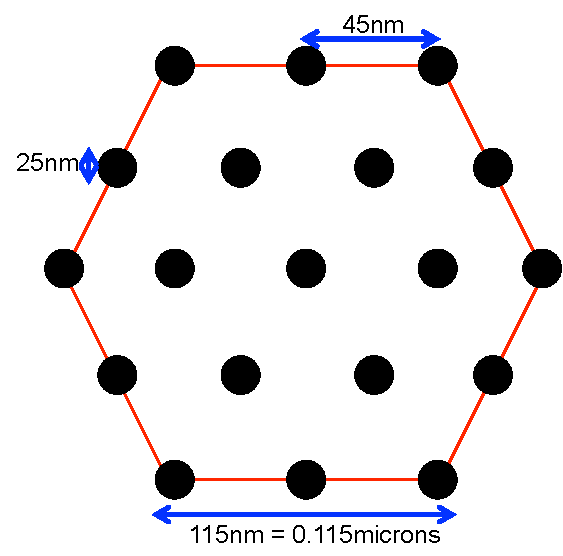
\includegraphics[height=5cm]{figure/microtubule_bundle.pdf} 
\end{array}
$
\end{center}
\caption{\label{fig:microtubule_bundle} Cross-section of microtubule bundle based on dimensions from Ref.\ \citenum{Peter:2012fc}. Diameter of a microtubule (black dot) is 25nm and edge-to-edge spacing between microtubules is 20nm. Figure is not drawn to scale. }
\end{figure}
%

%=========================================================================================================
\subsection{Multi-scale Implementation via AMSI}
\textcolor{red}{Bill can briefly describe implementation of AMSI here.}

%%%%%%%%%%%%%%%%%%%%%%%%%%%%%%%%%%%%%%%%%%%%%%%%%%%%%%%%%%%%%%%%%%%%%%
\section{Results and Discussion}
To gain insight about the interactions within innervated collagenous tissue, we examine the mechanical behavior of our embedded neuron model by deforming the surrounding collagen gel under different conditions. The effect of adjusting cell body stiffness is investigated by considering different values of $a$ in Eq.\ \eqref{eq:cellEA} (see Fig.\ \ref{fig:analysis_schematic}(b) for axial Young's modulus for $a=30$), while the effect of load direction is explored by considering different loading angles (see Fig.\ \ref{fig:analysis_schematic}(a)). 
%
%image for axial young's modulus from N2P178/3-Neuron_FT folder
\begin{figure}[ht]
\begin{center}
$
\begin{array}{cc}
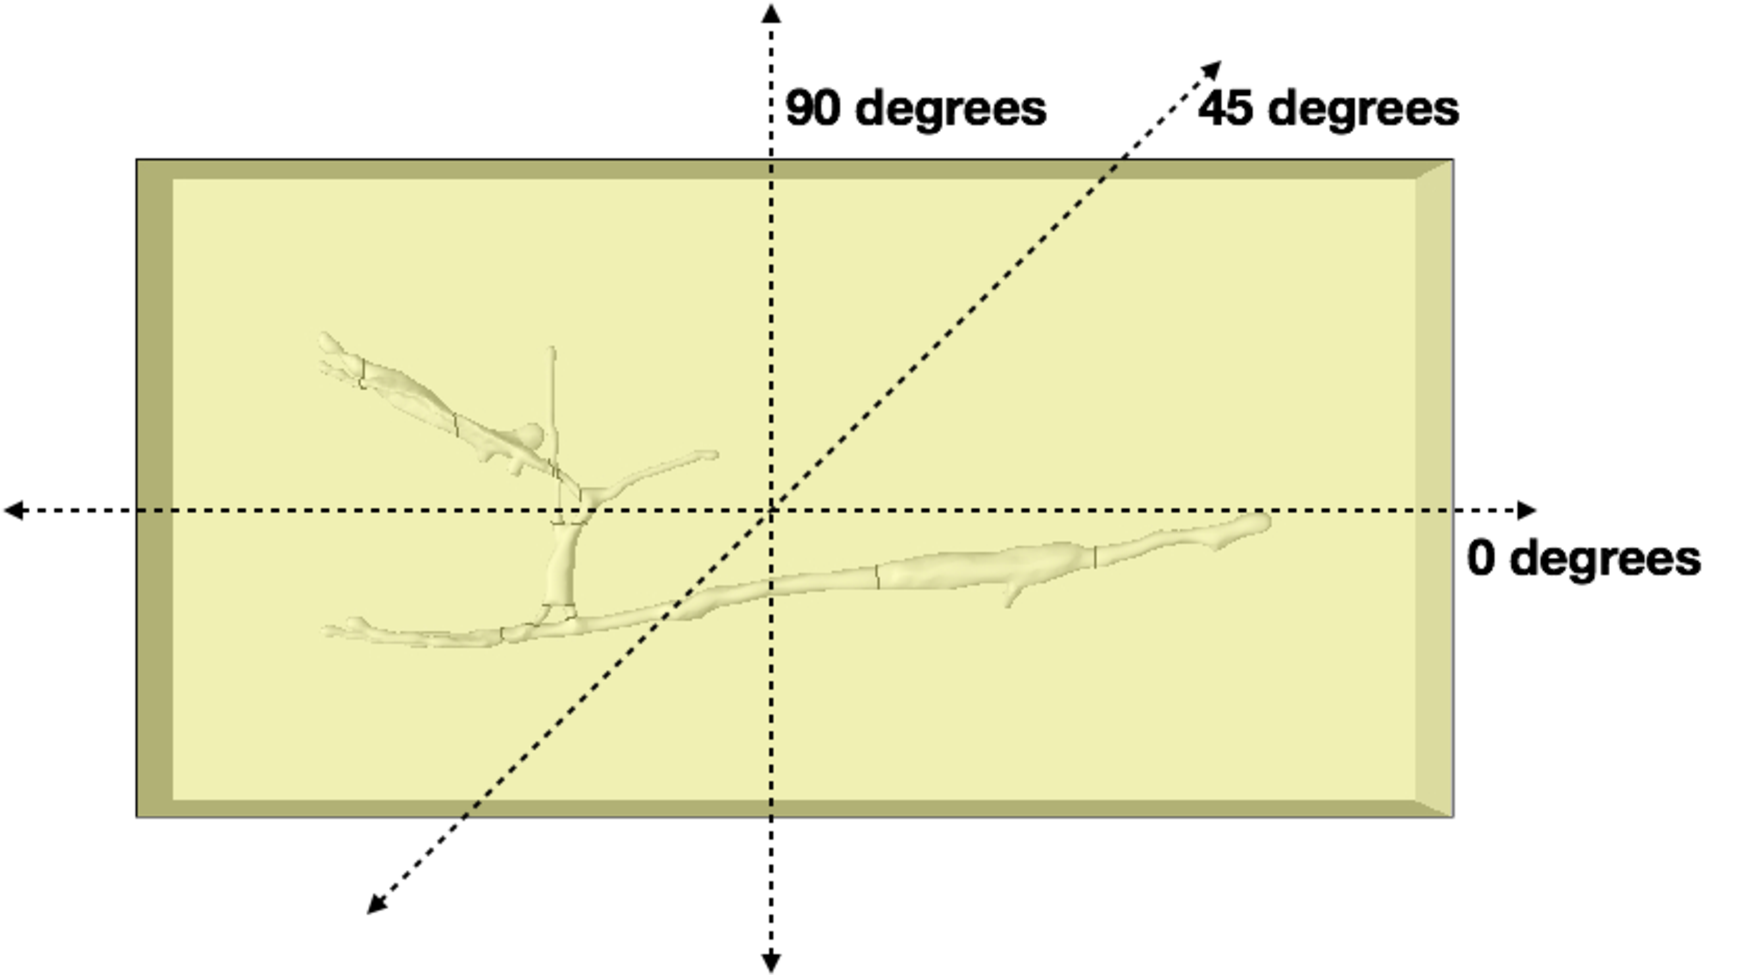
\includegraphics[height=4cm]{figure/AngleLoadingSchematic.pdf} &
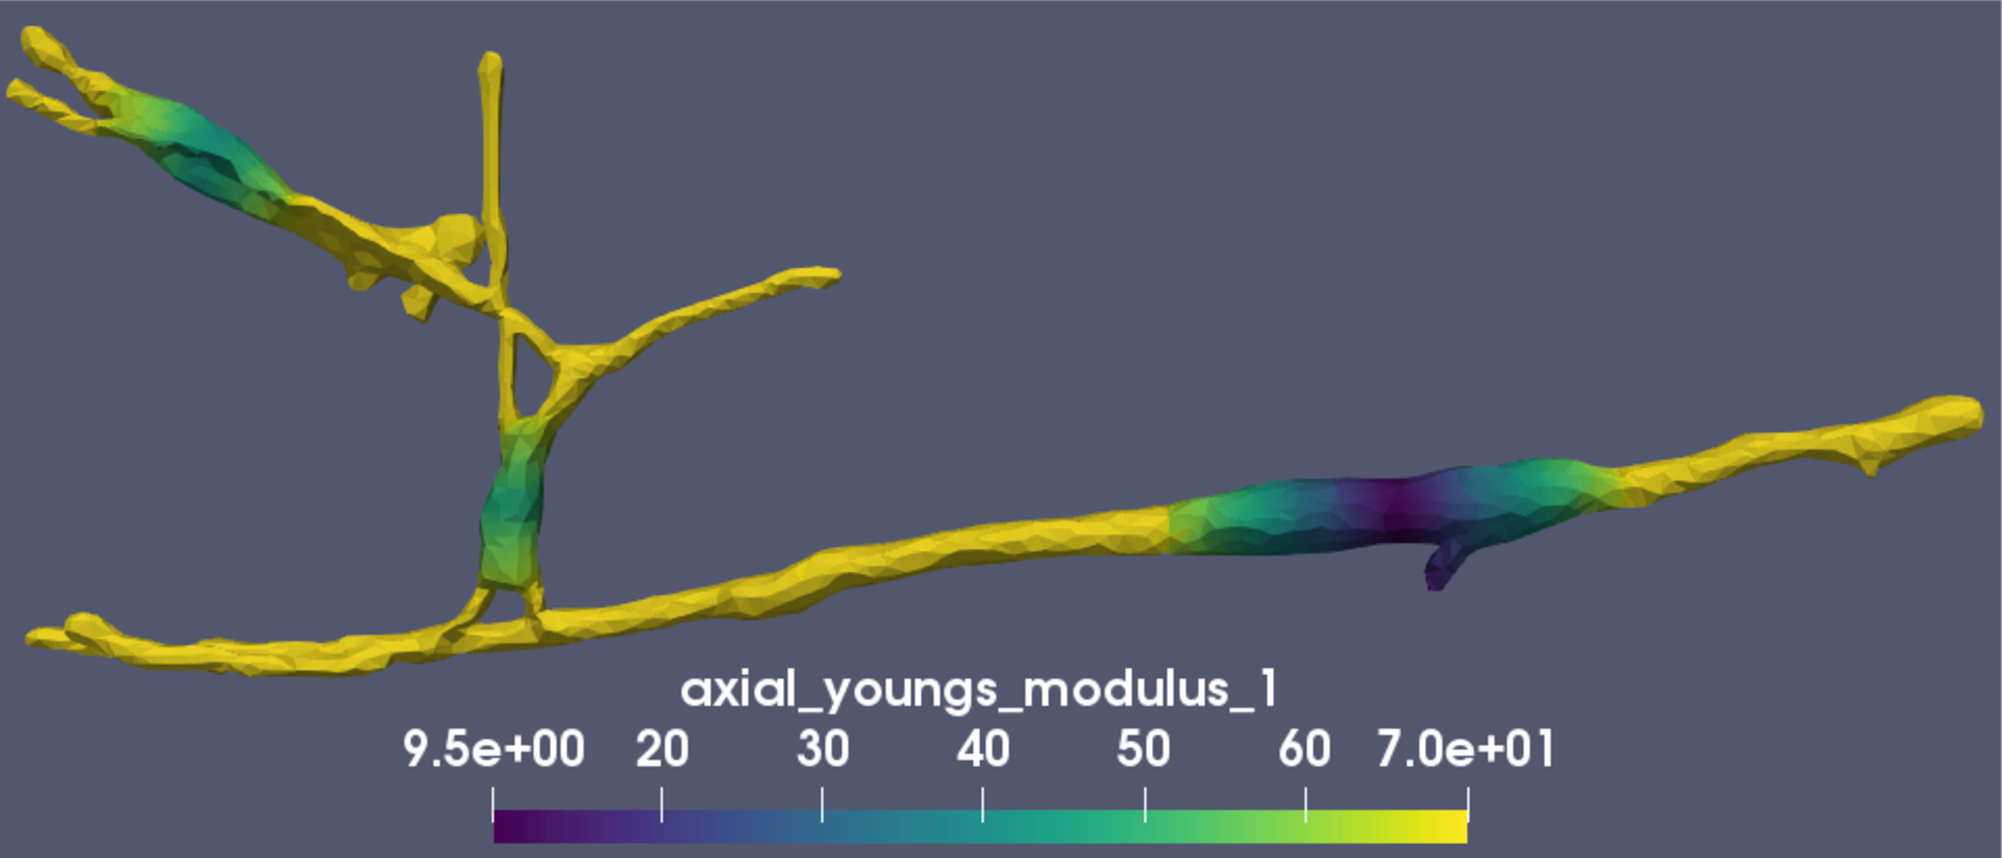
\includegraphics[height=3.5cm]{figure/axial_youngs_modulus_a30.pdf} \\
(a) & (b)
\end{array}
$
\end{center}
\caption{\label{fig:analysis_schematic} (a) Schematic showing load directions corresponding to 0 (solid black arrows), 45 (dotted arrows), and 90 (stripped arrows) degrees relative to the neuron structure. (b) Plot of axial Young's modulus for $a=30$ in Eq.\ \eqref{eq:cellEA} and $E_A=70$ kPa.}
\end{figure}
%
The strain distribution in the neuron is analyzed to identify loading conditions that may lead to neuronal damage. A cumulative distribution function (cdf) and its complement (ccdf) are employed for regions in the neuron that experience compressive and tensile strains, respectively. The cdf is defined as
%
\begin{equation}
cdf(x) = \sum_{i=1}^x f(i) = Pr[X \ge x],
\label{eq:cdf}
\end{equation}
%
where $f$ is a probability density function and $X$ is a random variable (i.e., a measure of strain). Equation \ref{eq:cdf} can be interpreted as measuring the probability that a region experiences a strain of \textit{at most} $x$. Such an interpretation is most suitable for compressive strains, which are negative in value. On the other hand, the complement of Eq.\ \eqref{eq:cdf} is
%
\begin{equation}
1 - cdf(x) = 1 - \sum_{i=1}^x f(i) = 1 - Pr[X \le x],
\label{eq:ccdf}
\end{equation}
%
and is the probability that a region experiences a strain of \textit{at least} $x$. Such an interpretation is suitable for tensile strains, which are positive in value. In our analysis, loads of up to 16$\%$, which is the pain threshold for ligament stretch \cite{Zhang:2016ga}, are considered. 

%=========================================================================================================
\subsection{Effect of Changing Cell Body Stiffness}
In our model, the cell body stiffness along the axial direction of adjacent axons depends on how quickly the microtubules in the neuron transition from aligned in the axon to unaligned in the cell body. The transition from aligned to unaligned is characterized by the variable $a$ in Eq.\ \eqref{eq:cellEA}. Therefore, the effect of such a transition from axon to microtubule on the overall mechanical behavior of the neuron can be explored by adjusting the value of $a$ in Eq.\ \eqref{eq:cellEA}. In this section three values of $a$ are considered: $a=$ 28, 30, and 50. A larger value of $a$ represents a more rapid transition from aligned to unaligned results in a softer cell body in the axial direction. The distributions of the maximum principal strain, $\epsilon_{\text{max}}$ for different cell body stiffnesses (different values of $a$) are plotted in Fig.\ \ref{fig:neuron_ccdf_vary_a}.
%
% Figures generated in N2P178/6-Neuron_CellStiffness/MaxPrnStrn folder
\begin{figure}[ht]
\begin{center}
$
\begin{array}{ccc}
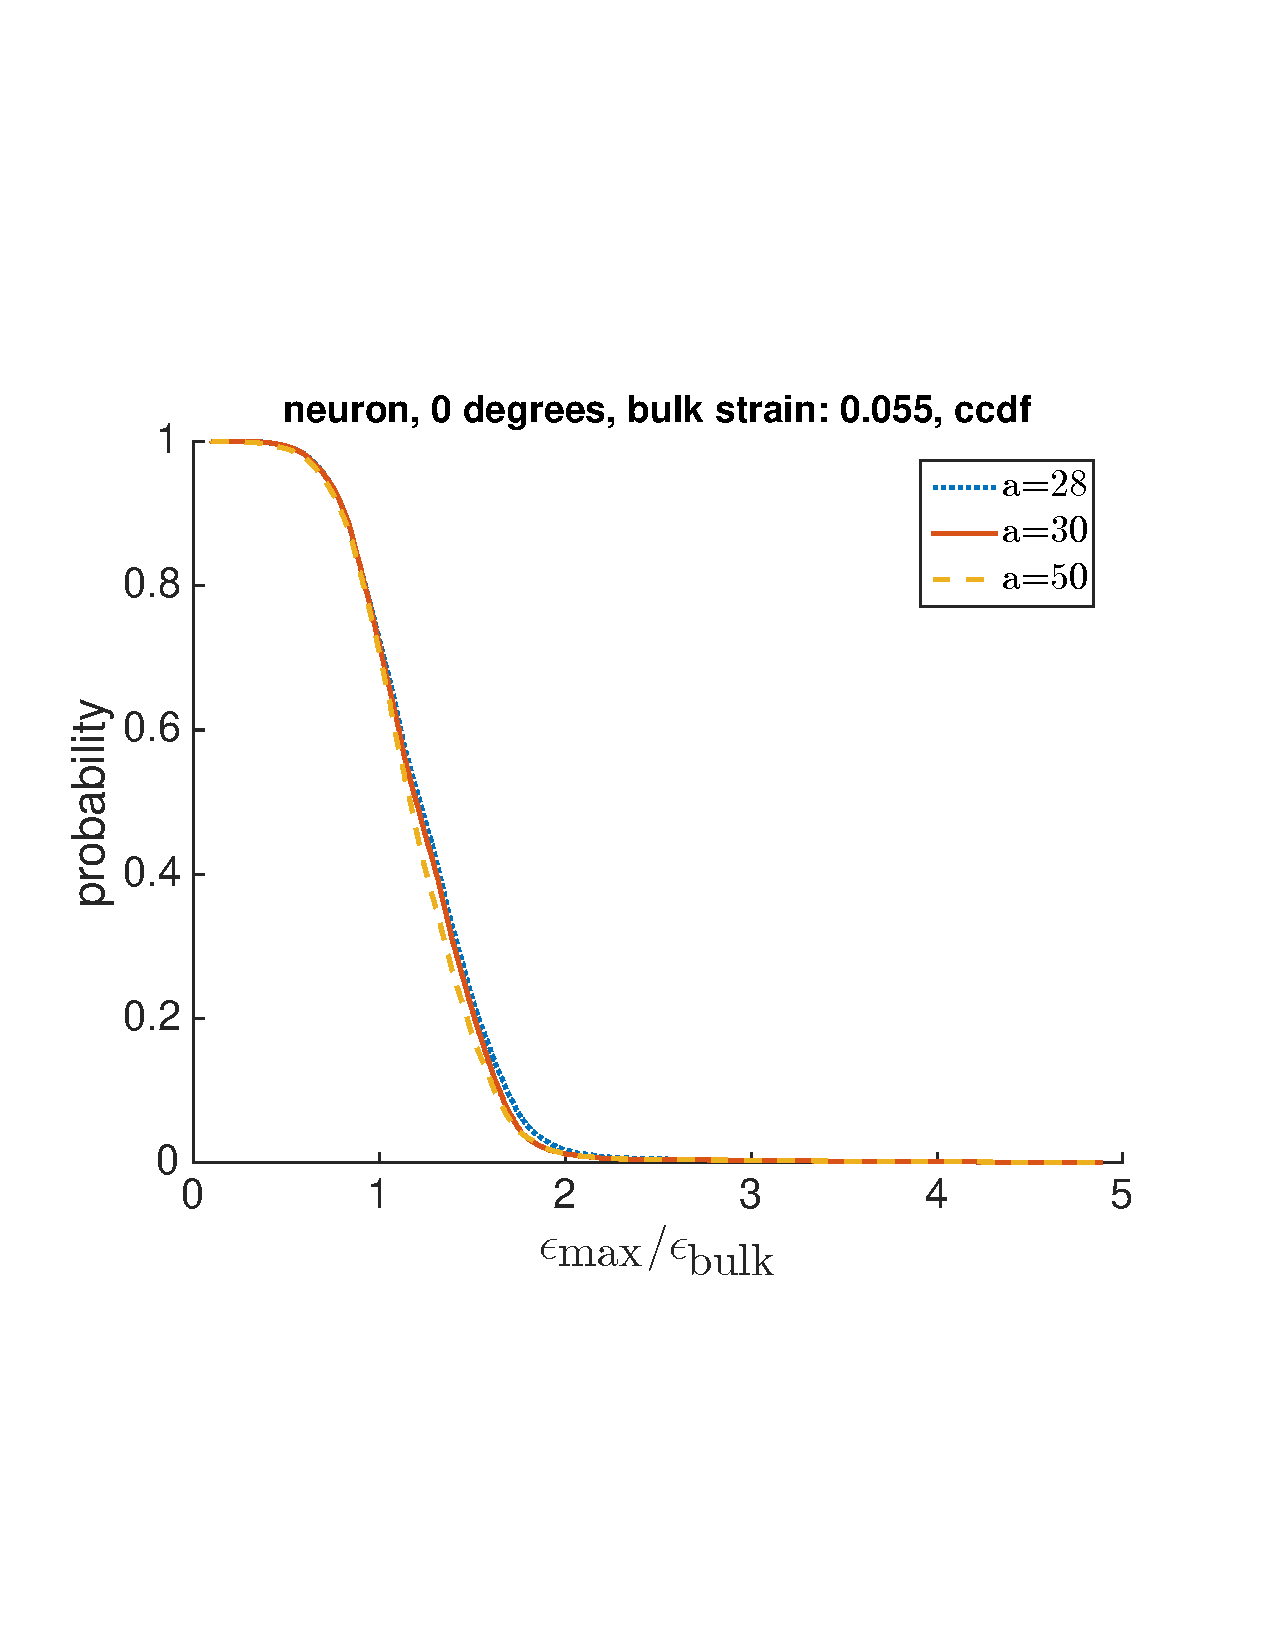
\includegraphics[height=4.5cm]{figure/rot0_FT_128_1920_ccdf_neuron_compare_a_strn0_055.pdf} &
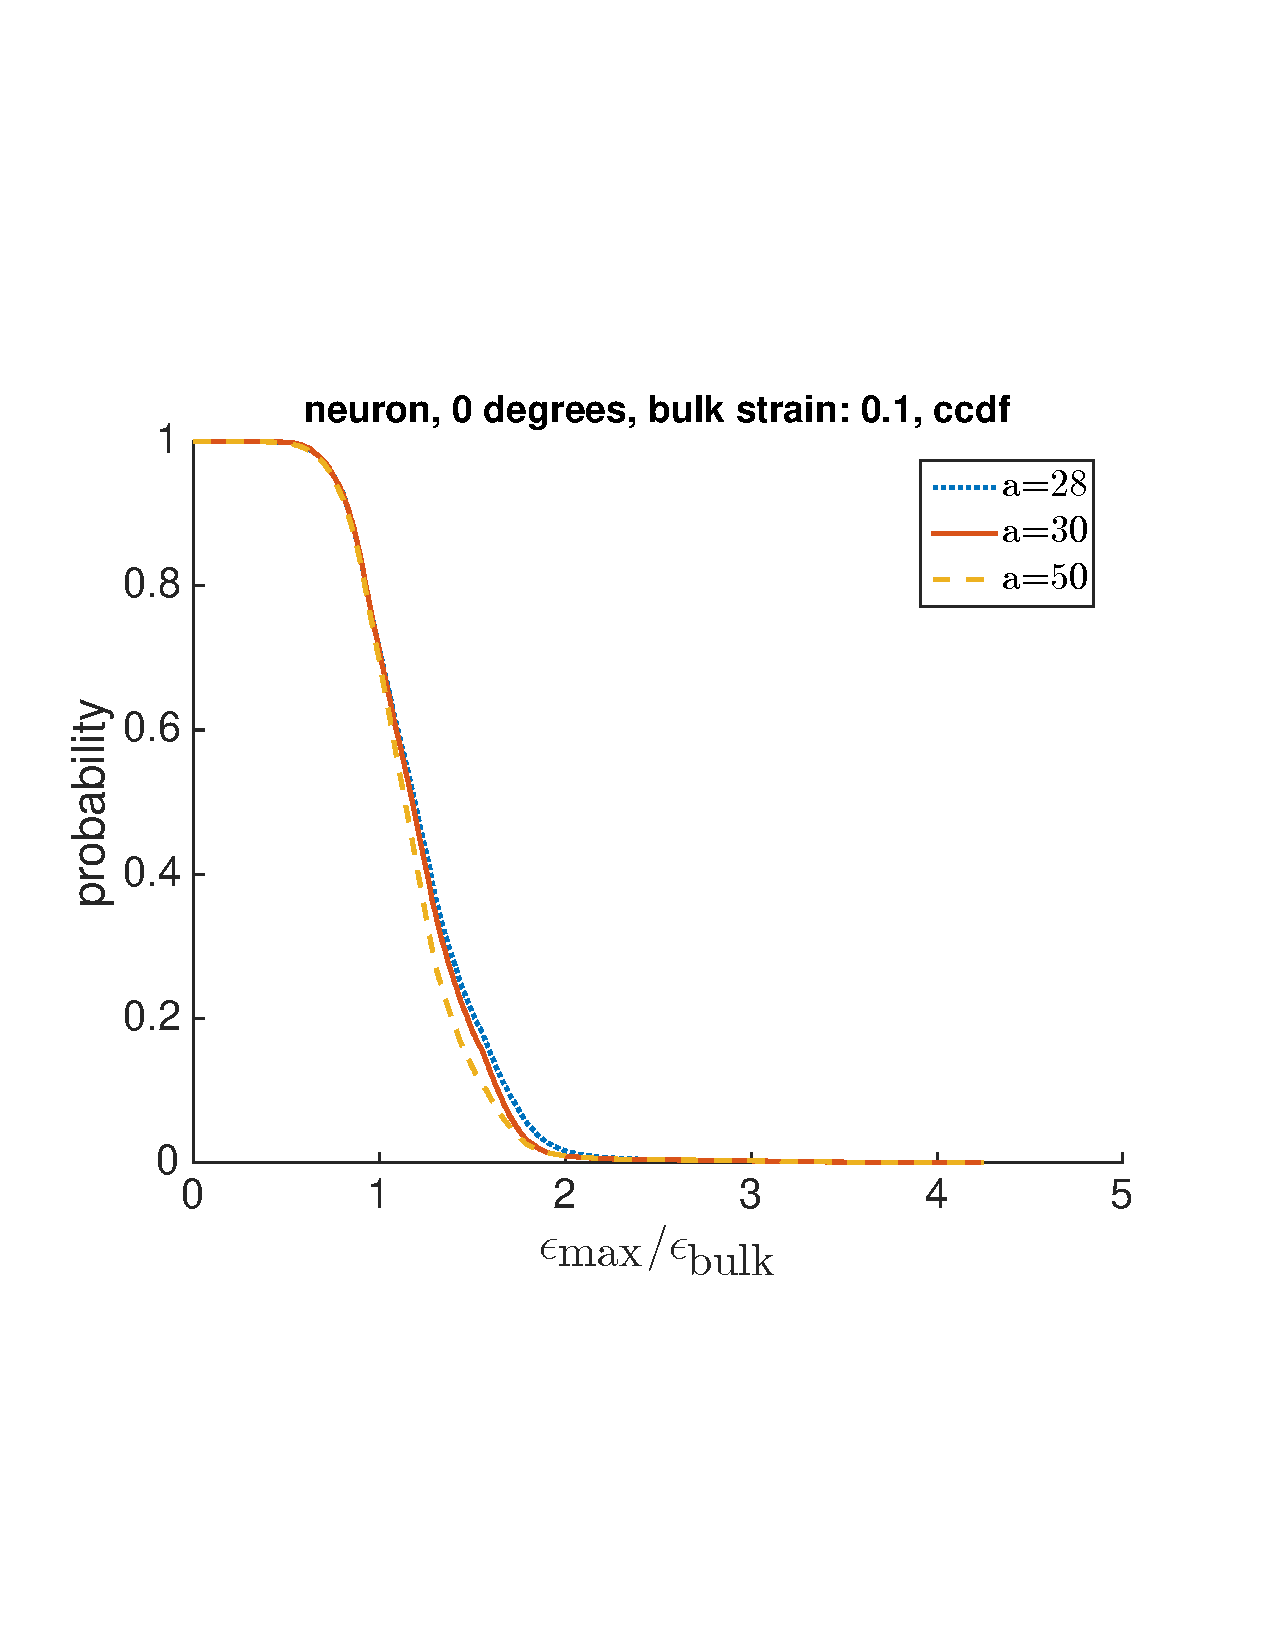
\includegraphics[height=4.5cm]{figure/rot0_FT_128_1920_ccdf_neuron_compare_a_strn0_1.pdf} &
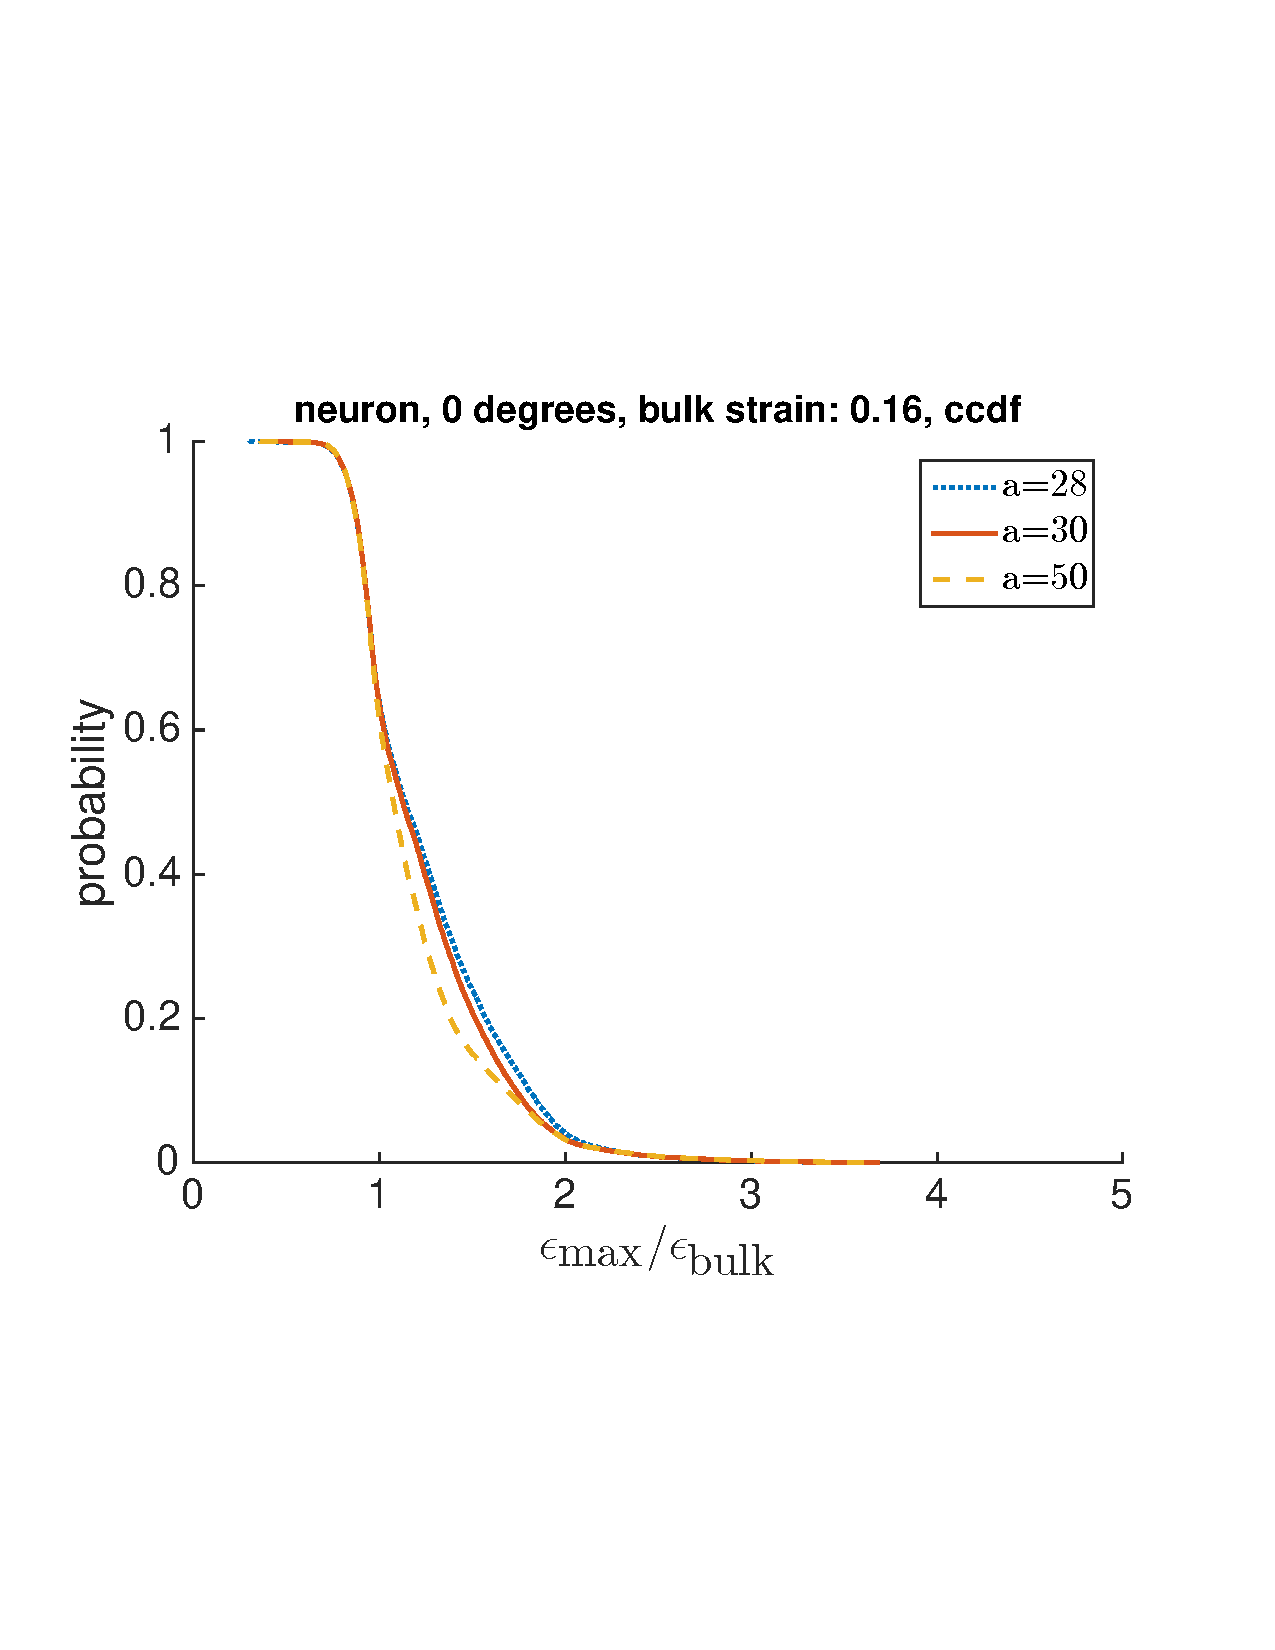
\includegraphics[height=4.5cm]{figure/rot0_FT_128_1920_ccdf_neuron_compare_a_strn0_16.pdf} \\
(a) & (b) & (c)
\end{array}
$
\end{center}
\caption{\label{fig:neuron_ccdf_vary_a} Distributions (ccdf) of maximum principal strain, $\epsilon_{\text{max}}$, in neuron for different cell body stiffnesses: a=28 (blue dotted line), 30 (red solid line), and 50 (dashed yellow line). Three different bulk strains are considered: $\epsilon_{\text{bulk}}=$ (a) 5.5$\%$, (b) 10 $\%$, and (c) 16$\%$. The $\epsilon_{\text{max}}$ values are normalized by the $\epsilon_{\text{bulk}}$. }
\end{figure}
%

As seen in Fig.\ \ref{fig:neuron_ccdf_vary_a}, increasing the cell body stiffness (increasing $a$) causes the distribution to shift to the left corresponding to a relatively stiffer neuron. The variations in the overall strain distribution caused by varying the cell body stiffness is fairly small \textcolor{red}{[Does this small variation mean anything physical?]}. The strain distributions of regions corresponding to cell bodies and axons are plotted in Fig.\ \ref{fig:rgns_ccdf_vary_a}. 
%
% Figures generated in N2P178/6-Neuron_CellStiffness/MaxPrnStrn folder
\begin{figure}[ht]
\begin{center}
$
\begin{array}{ccc}
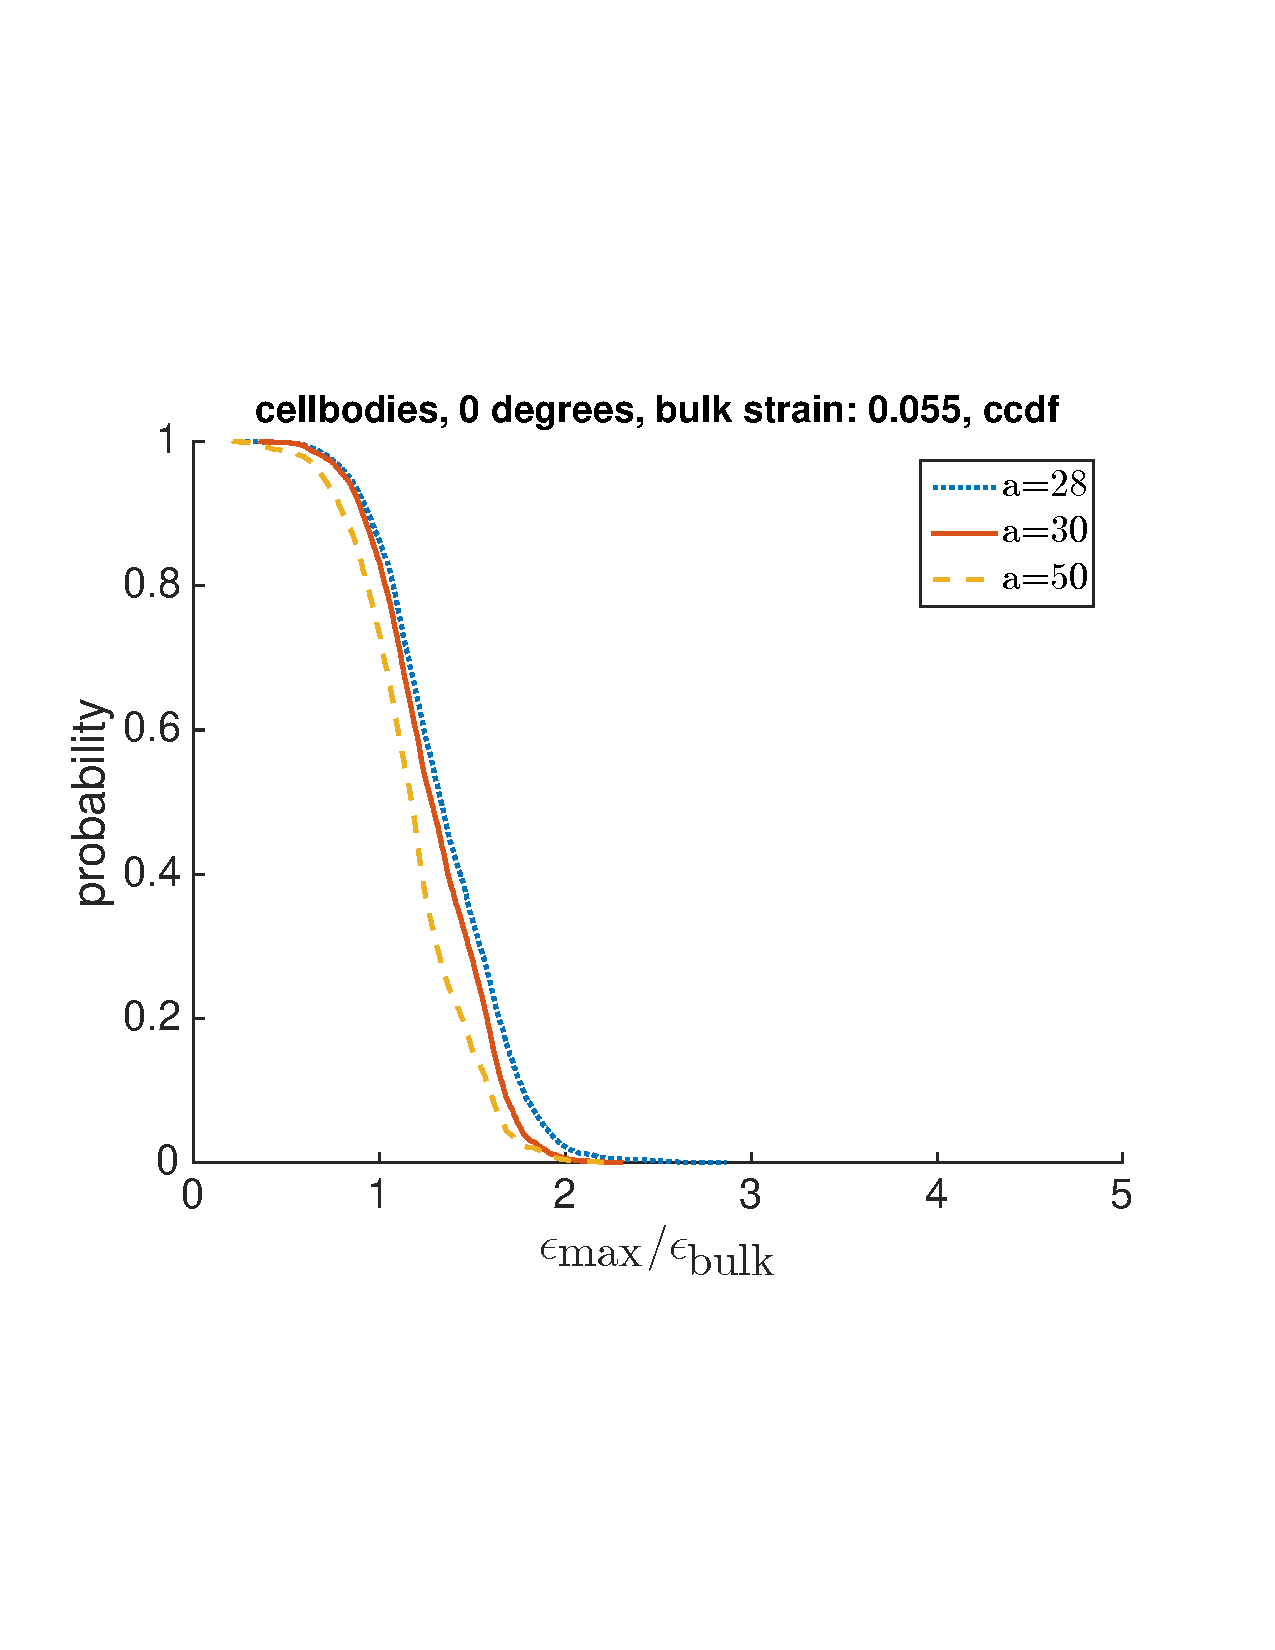
\includegraphics[height=4.5cm]{figure/rot0_FT_128_1920_ccdf_cellbodies_compare_a_strn0_055.pdf} &
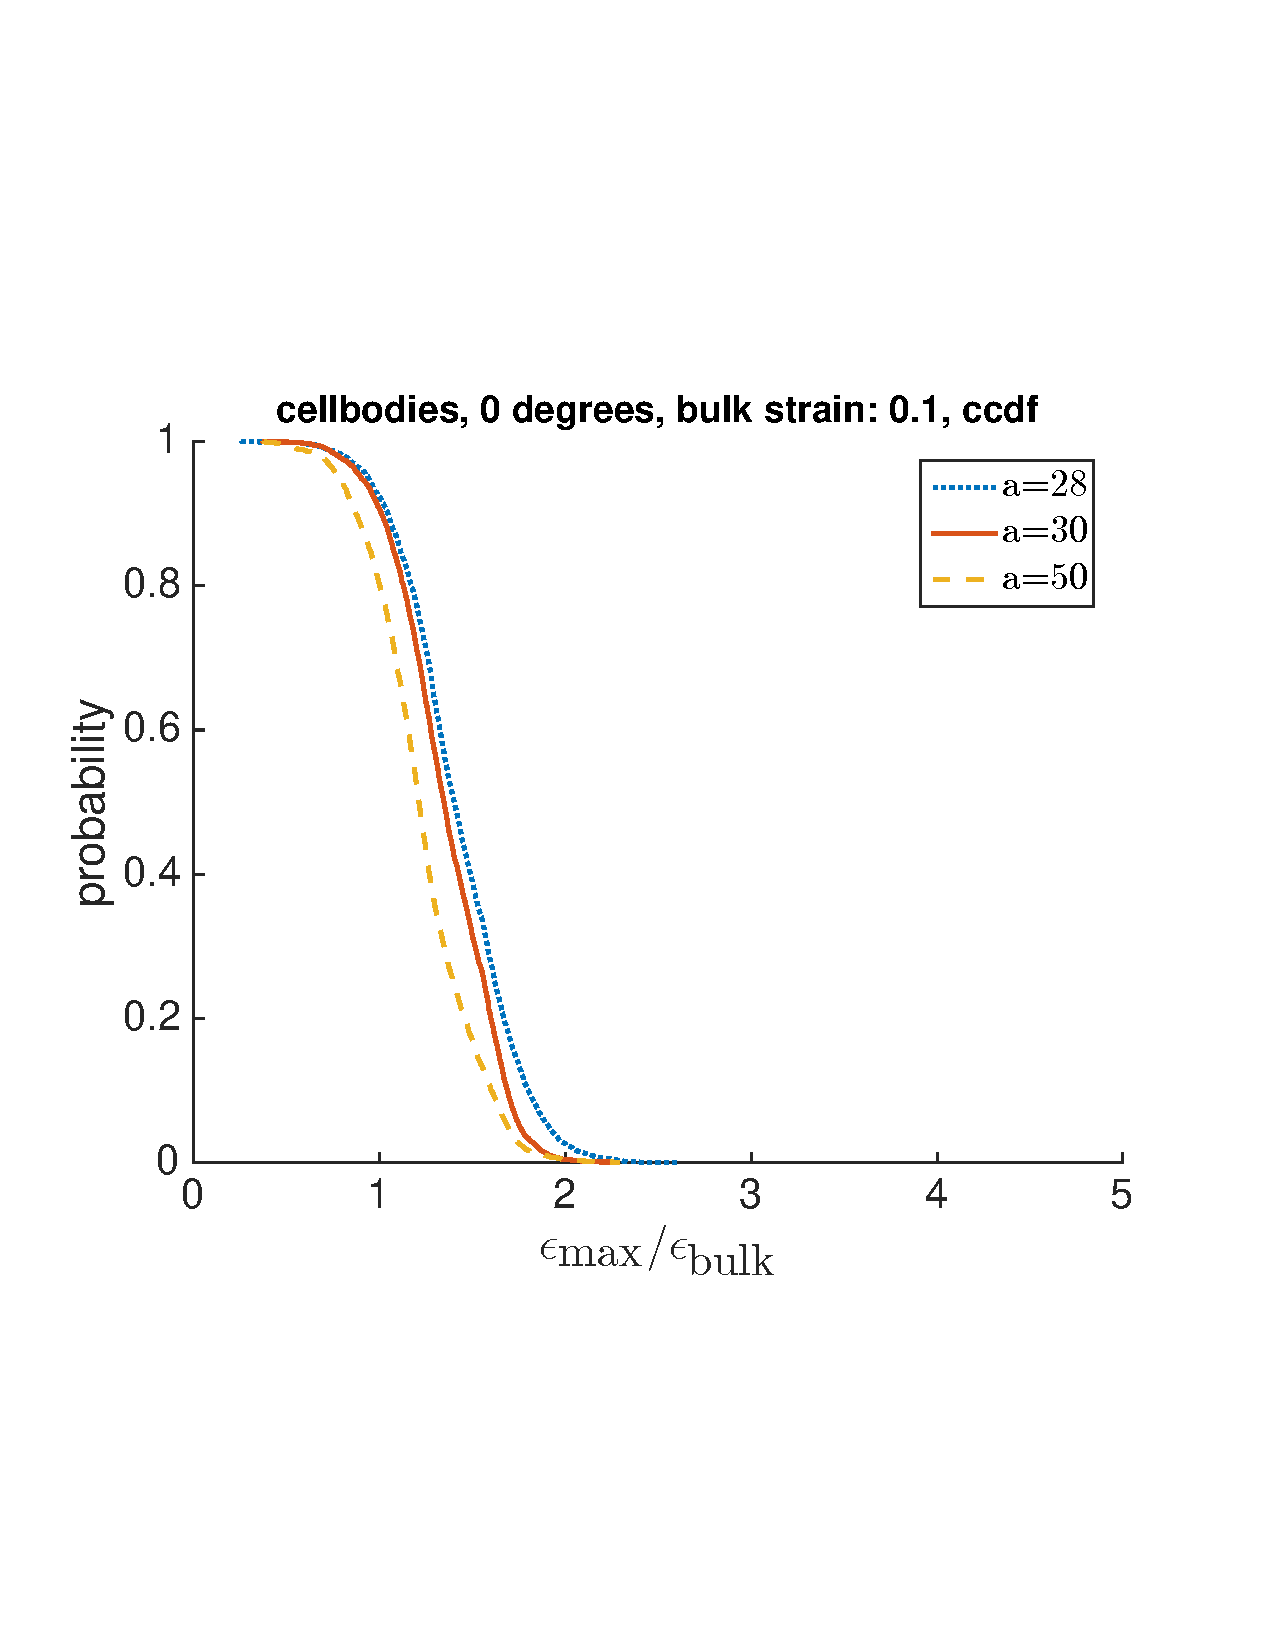
\includegraphics[height=4.5cm]{figure/rot0_FT_128_1920_ccdf_cellbodies_compare_a_strn0_1.pdf} &
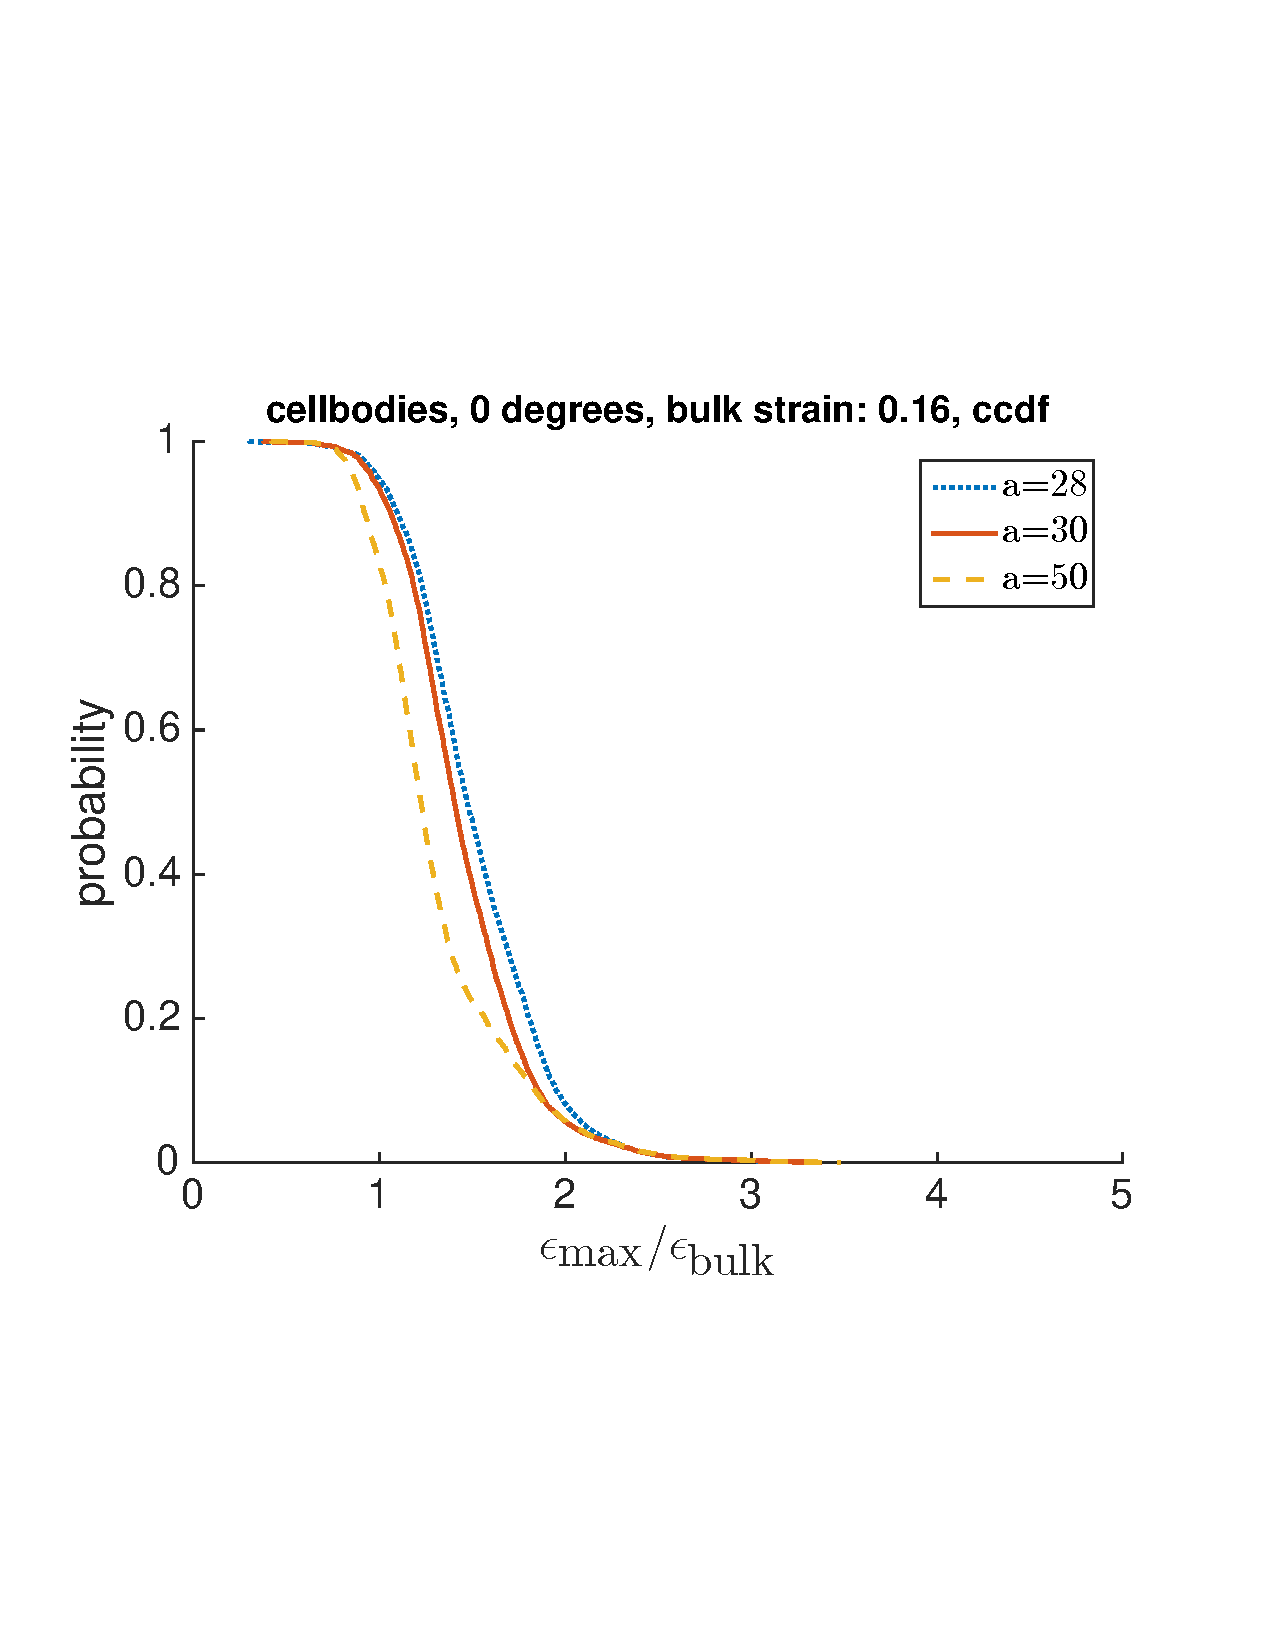
\includegraphics[height=4.5cm]{figure/rot0_FT_128_1920_ccdf_cellbodies_compare_a_strn0_16.pdf} \\
(a) & (b) & (c) \\
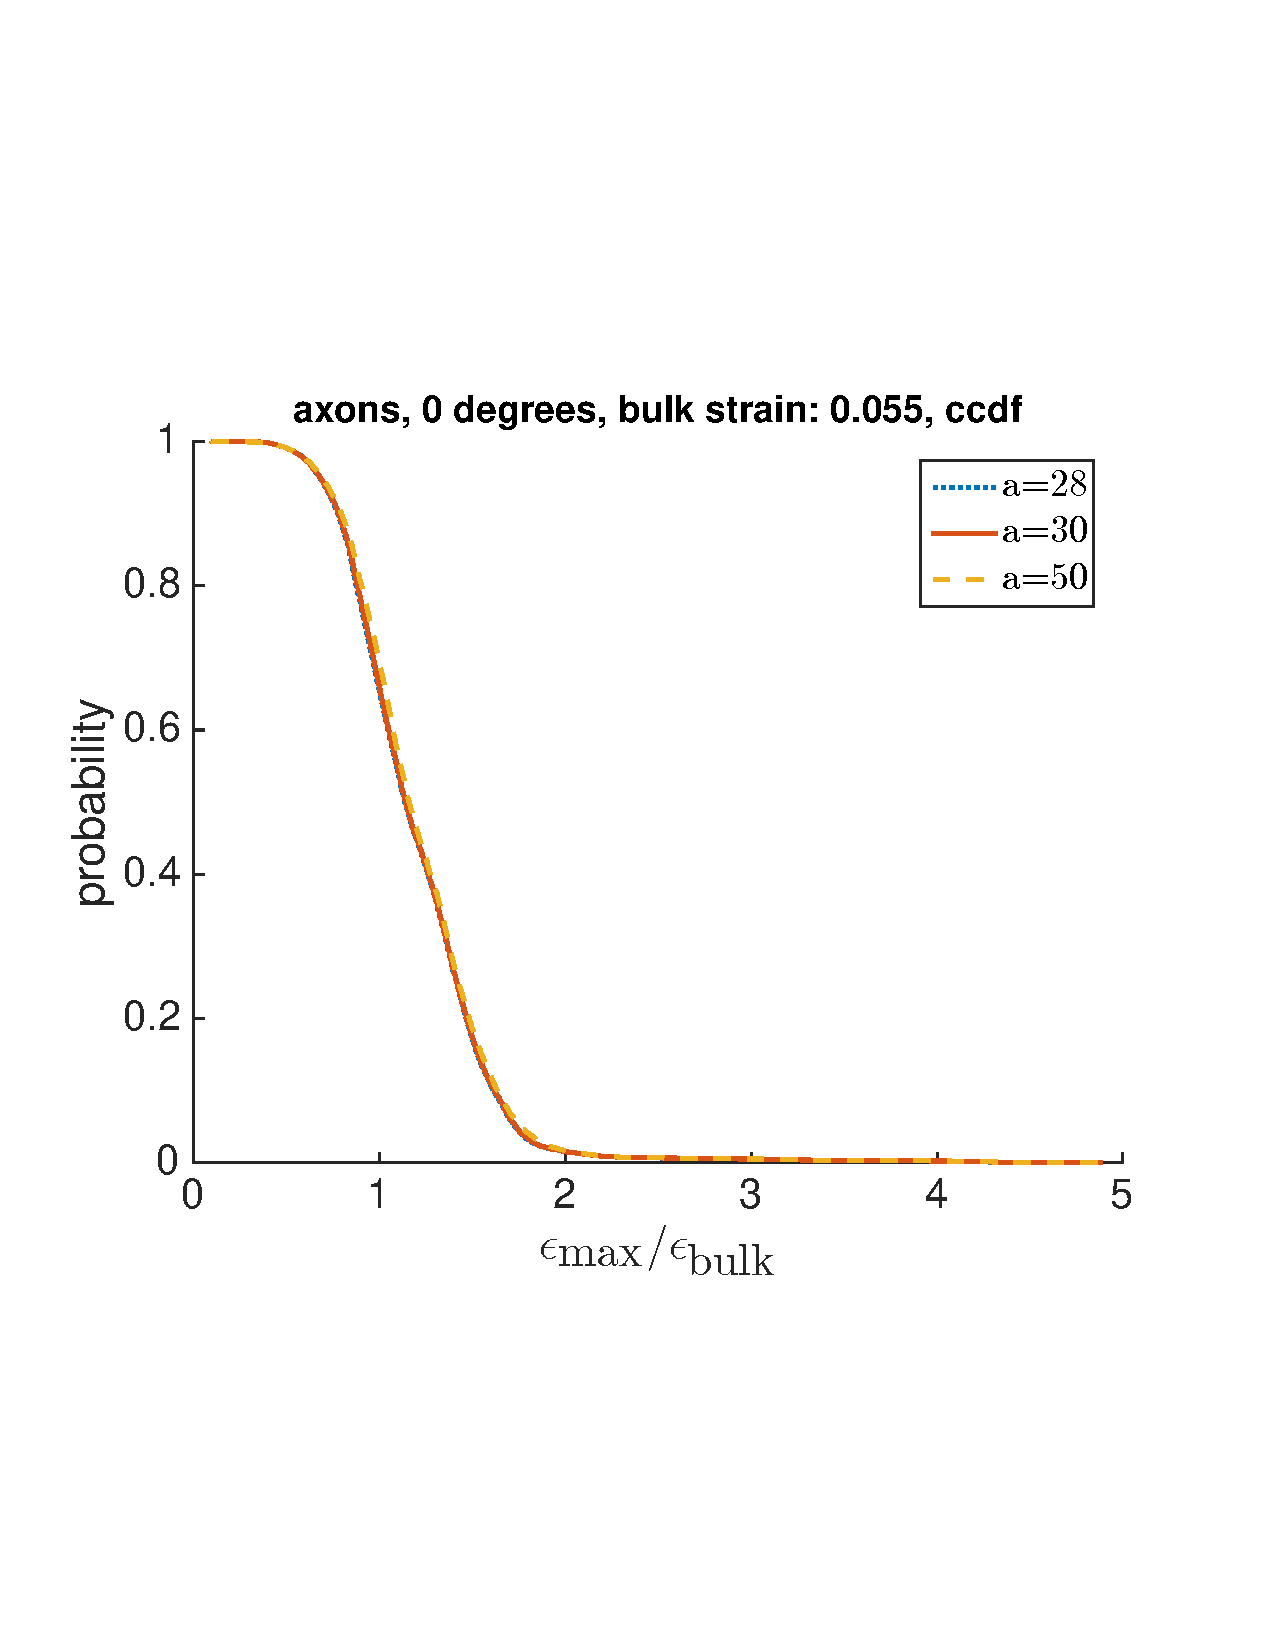
\includegraphics[height=4.5cm]{figure/rot0_FT_128_1920_ccdf_axons_compare_a_strn0_055.pdf} &
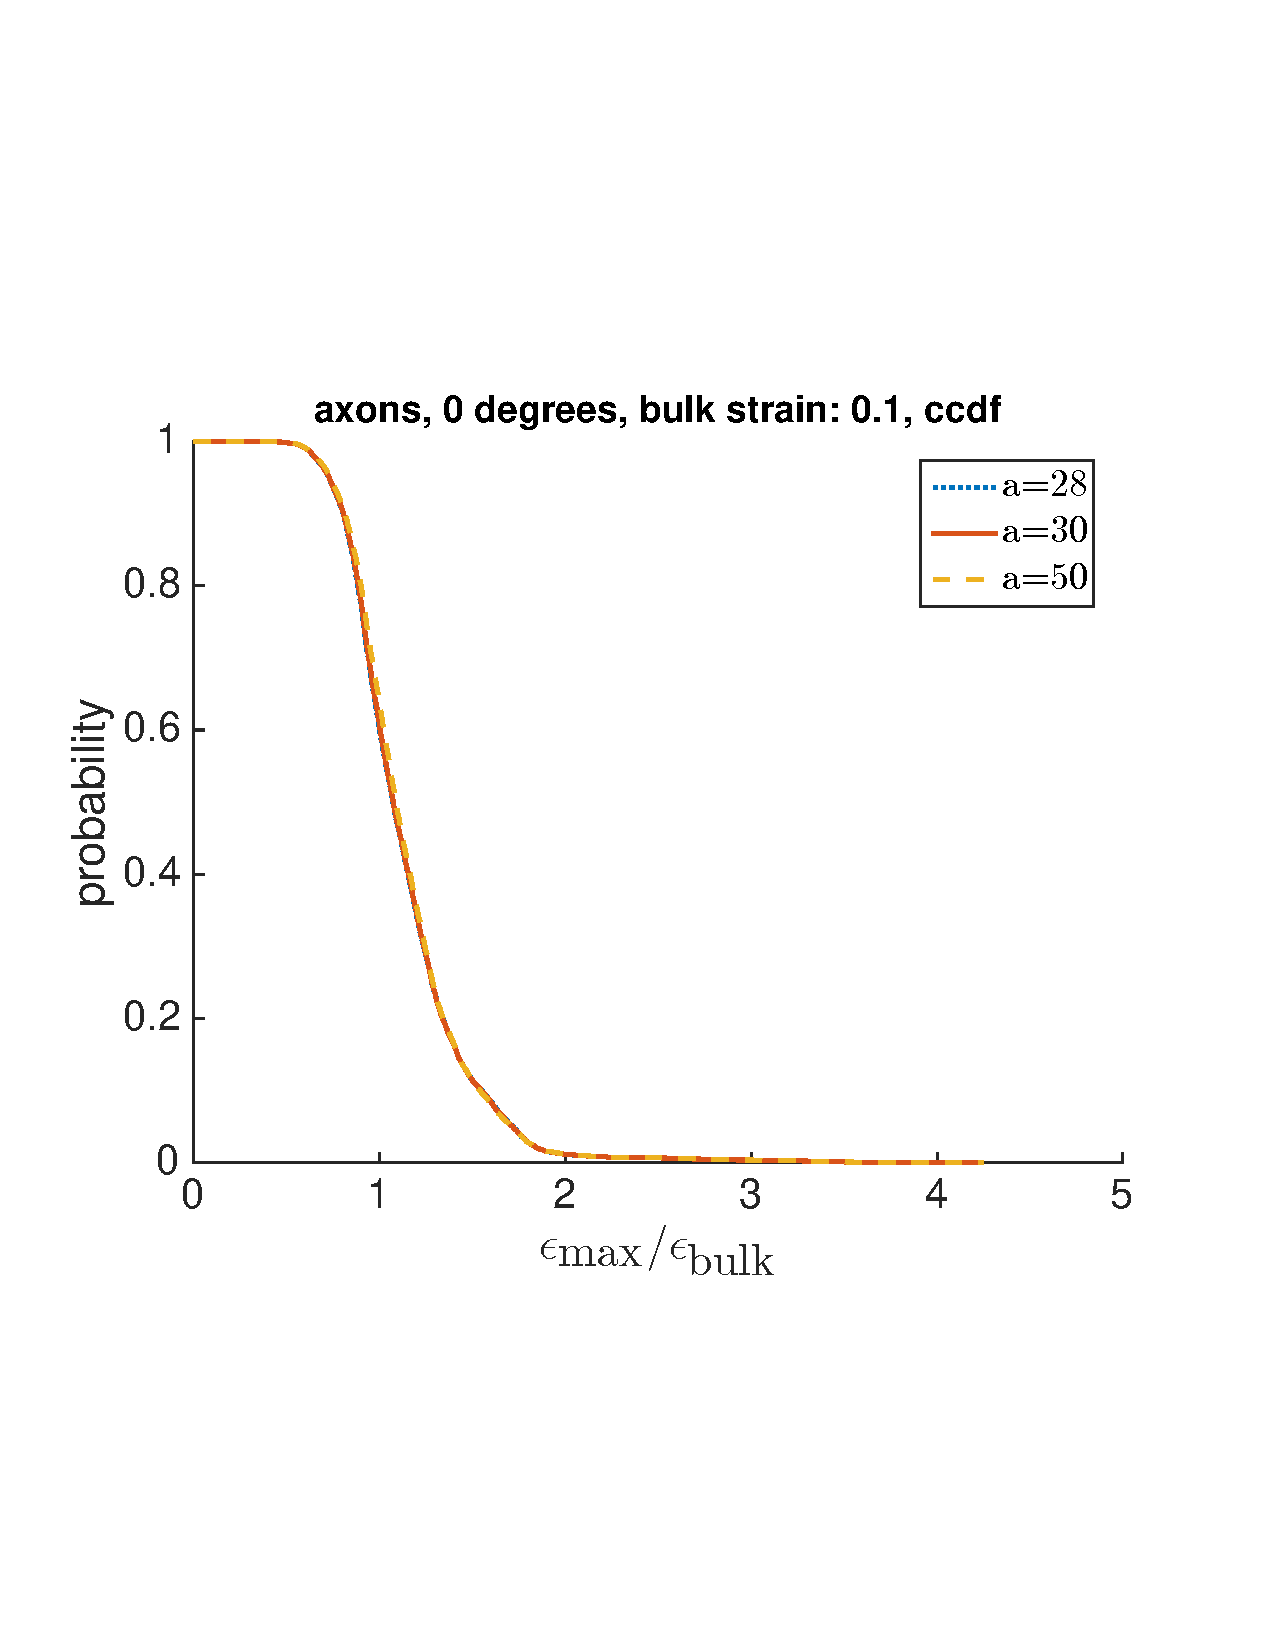
\includegraphics[height=4.5cm]{figure/rot0_FT_128_1920_ccdf_axons_compare_a_strn0_1.pdf} &
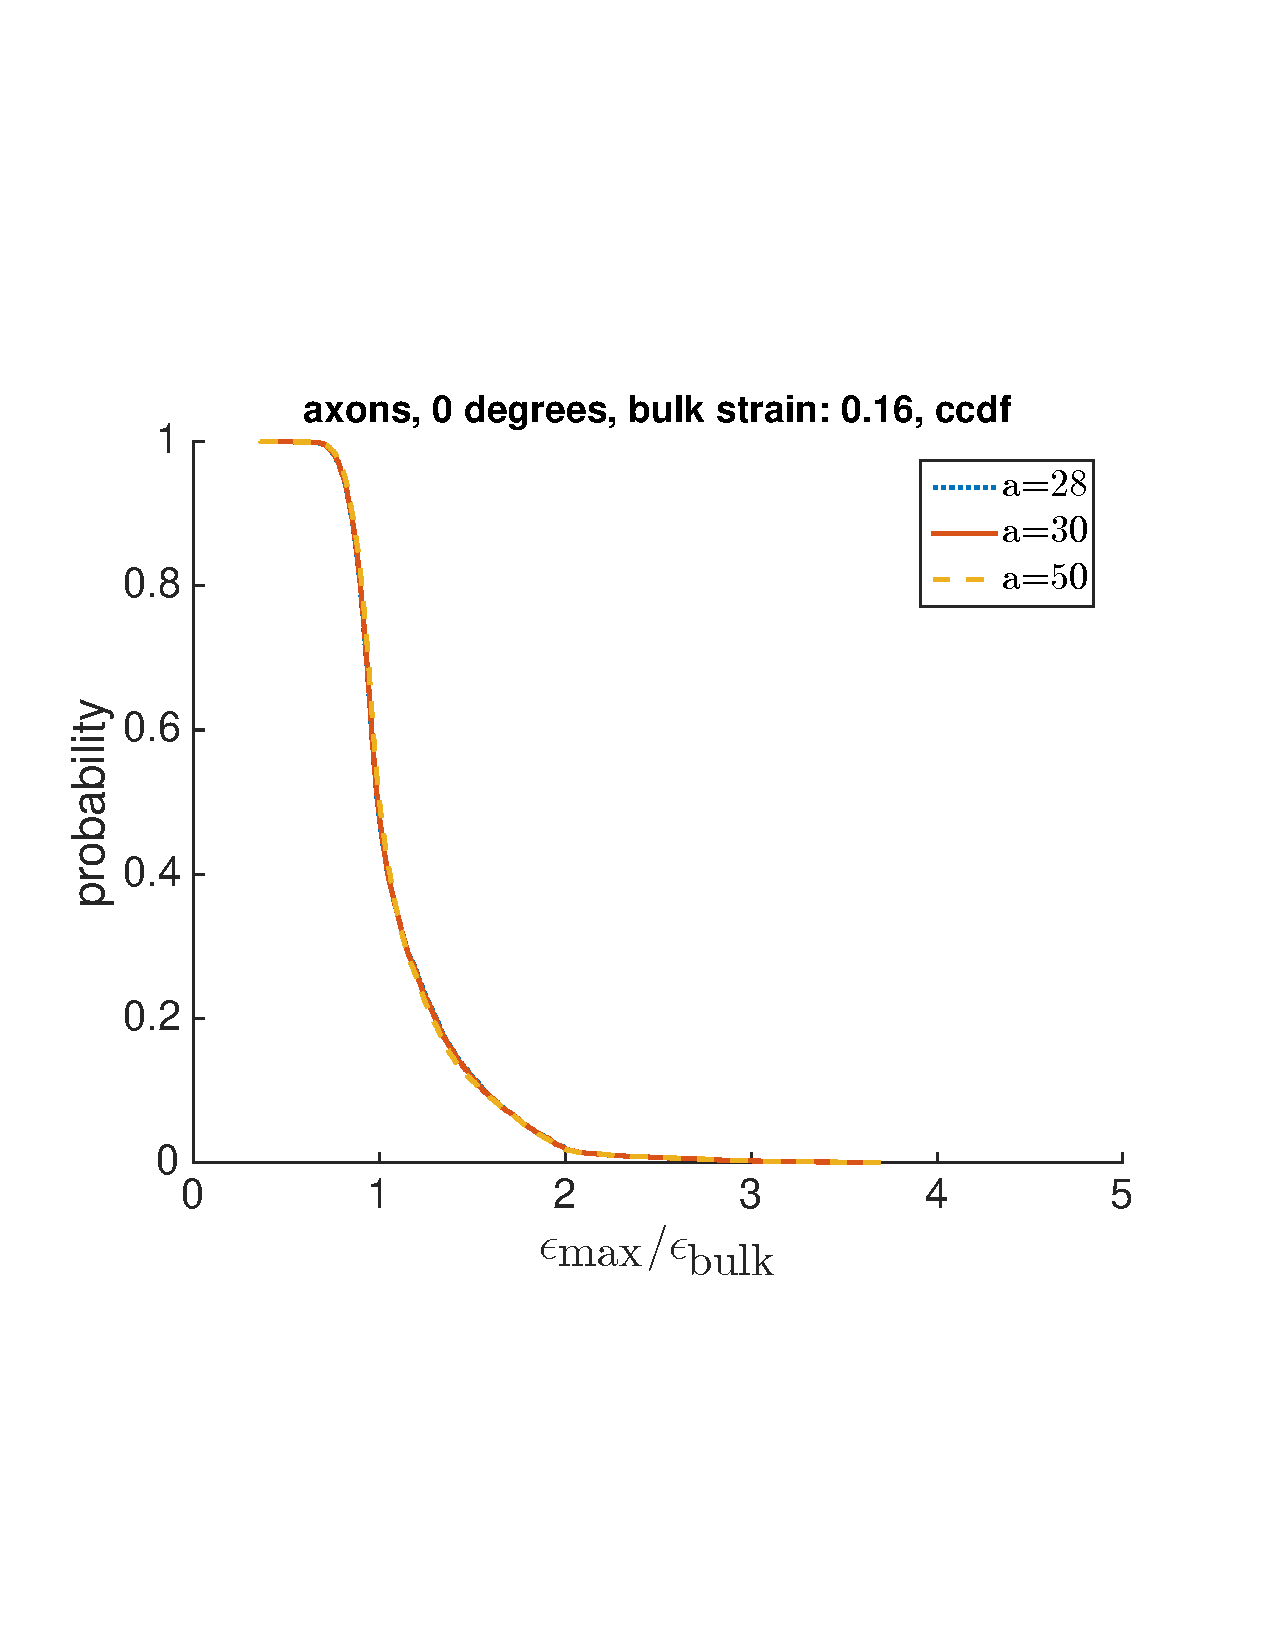
\includegraphics[height=4.5cm]{figure/rot0_FT_128_1920_ccdf_axons_compare_a_strn0_16.pdf} \\
(d) & (e) & (f)
\end{array}
$
\end{center}
\caption{\label{fig:rgns_ccdf_vary_a} Distributions (ccdf) of maximum principal strain, $\epsilon_{\text{max}}$, in cell bodies (top row) and axons (bottom row) for different cell body stiffnesses: a=28 (blue dotted line), 30 (red solid line), and 50 (dashed yellow line). Three different bulk strains are considered: $\epsilon_{\text{bulk}}=$ (a,d) 5.5$\%$, (b,e) 10 $\%$, and (c,f) 16$\%$. The $\epsilon_{\text{max}}$ values are normalized by the $\epsilon_{\text{bulk}}$. }
\end{figure}
%

As seen in Fig.\ \ref{fig:rgns_ccdf_vary_a}, the slight variations seen in the overall strain distribution for the neuron (Fig.\ \ref{fig:neuron_ccdf_vary_a}) is entirely due to variations in the strain of the cell body: the strain distributions in the axons are identical for all values of $a$ considered. As seen in the neuron, the strain distribution for the cell bodies shift to the left corresponding to the stiffening of the cell body, which is consistent with using larger values of $a$. These results suggests that the effects of adjusting the cell body stiffness has only a minimal effect on the overall strain distribution in the neuron. \textcolor{red}{[Amplification increases with increasing bulk strain. This point is further explored in later sections below.]}

%=========================================================================================================
\subsection{Effect of Changing Load Direction}
In this section, the effect of changing the loading angle is explored for cell stiffness corresponding to $a$=30 in Eq.\ \eqref{eq:cellEA}. The three loading angles of 0, 45, and 90 degrees are shown in the schematic of Fig.\ \ref{fig:analysis_schematic}(a). Color maps of the maximum principal strain on the neuron structure for different loading angles are plotted in Fig.\ \ref{fig:neuron_MPS} for two different bulk strains.
%
% Images from N2P178/4-Neuron_FT_trcBC folder.
\begin{figure}[ht]
\begin{center}
$
\begin{array}{cc}
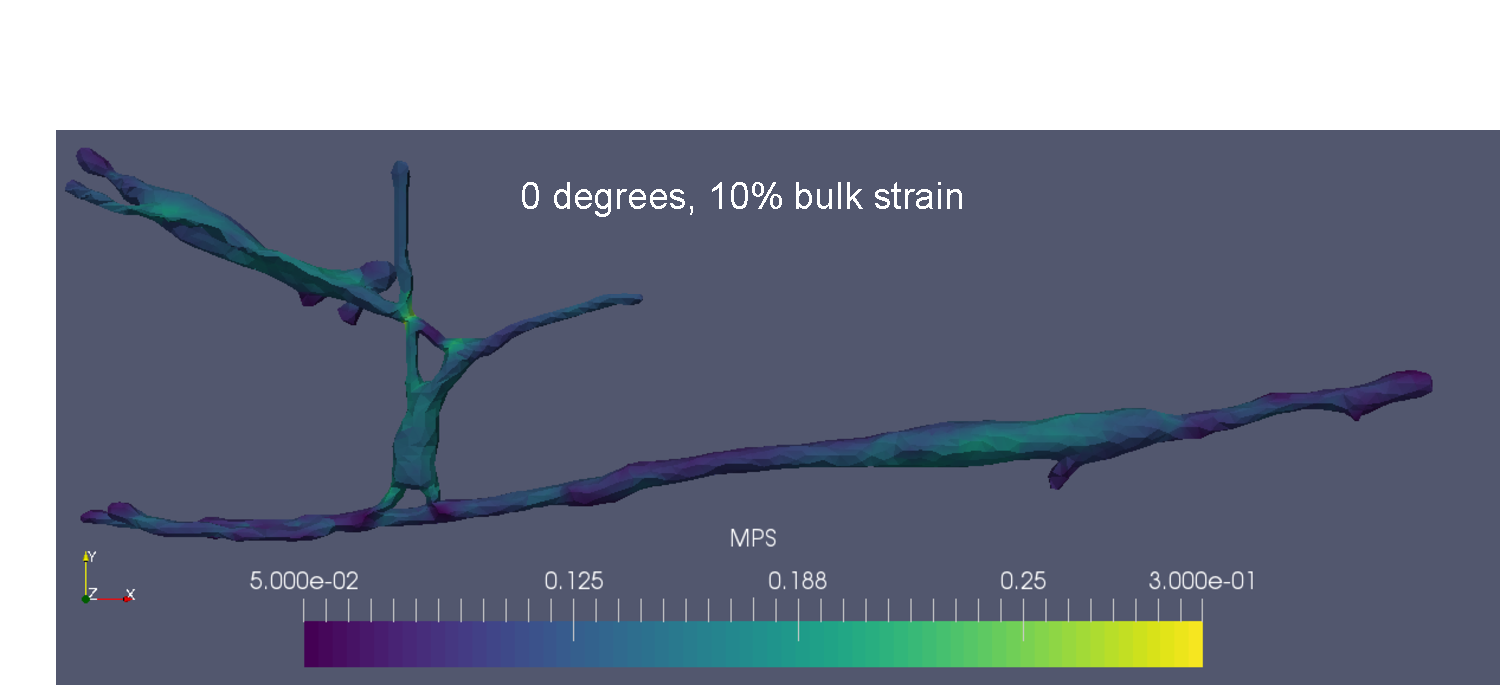
\includegraphics[width=8cm]{figure/MPS_rot0_strain10.pdf} & 
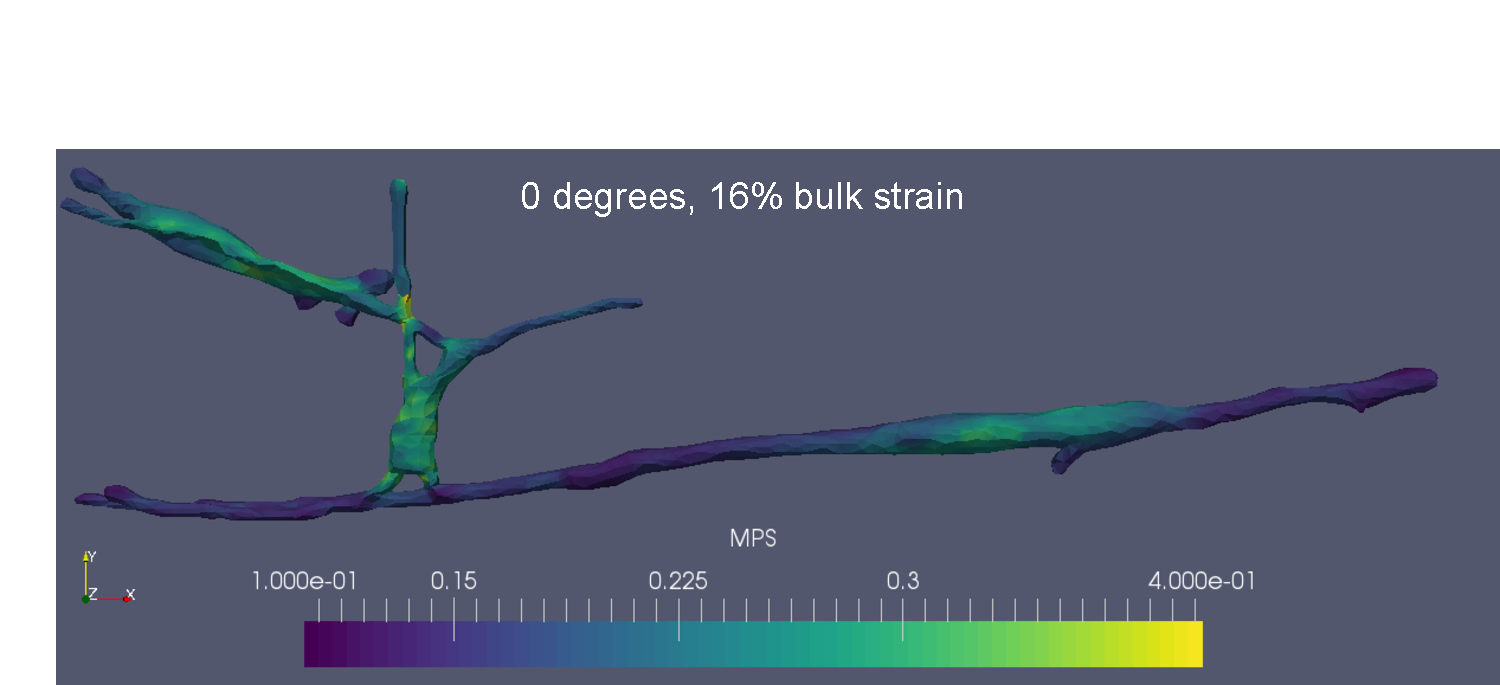
\includegraphics[width=8cm]{figure/MPS_rot0_strain16.pdf} \\
(a) & (b) \\ 
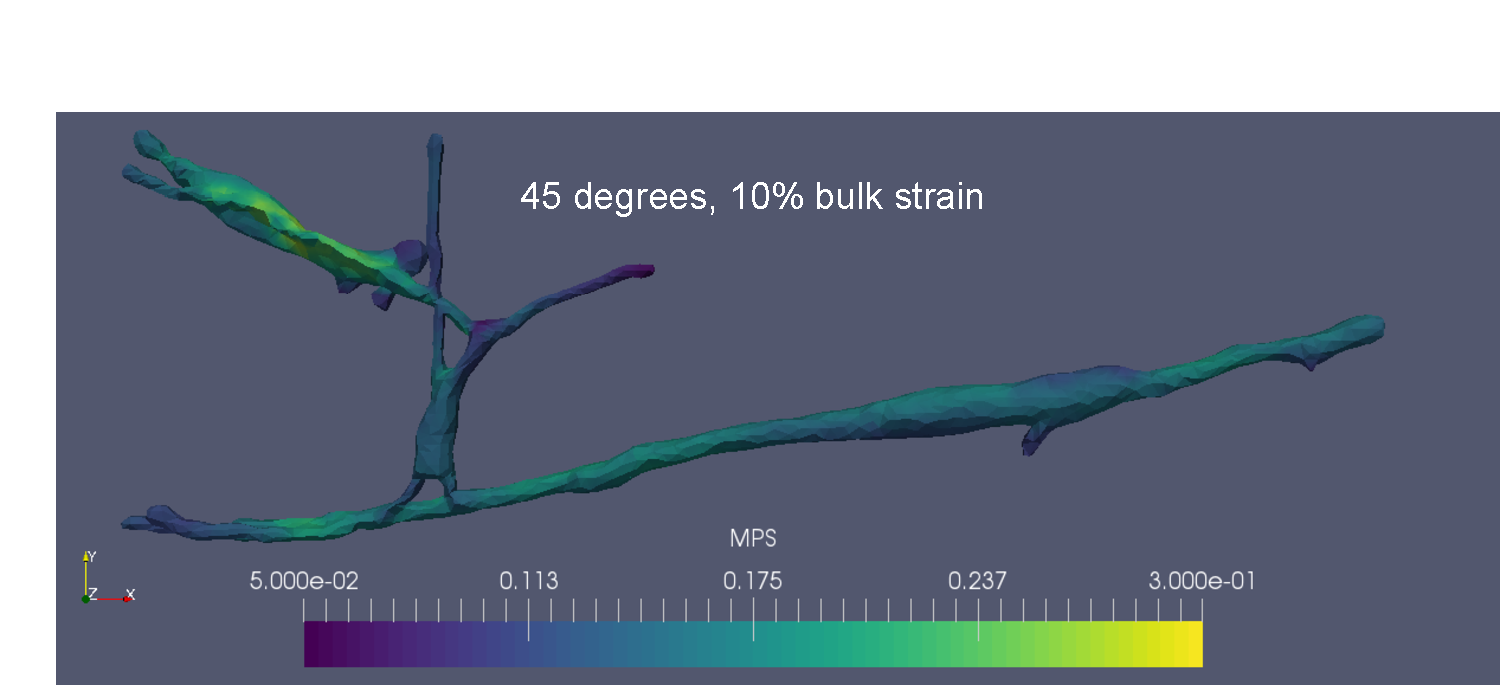
\includegraphics[width=8cm]{figure/MPS_rot45_strain10.pdf} &
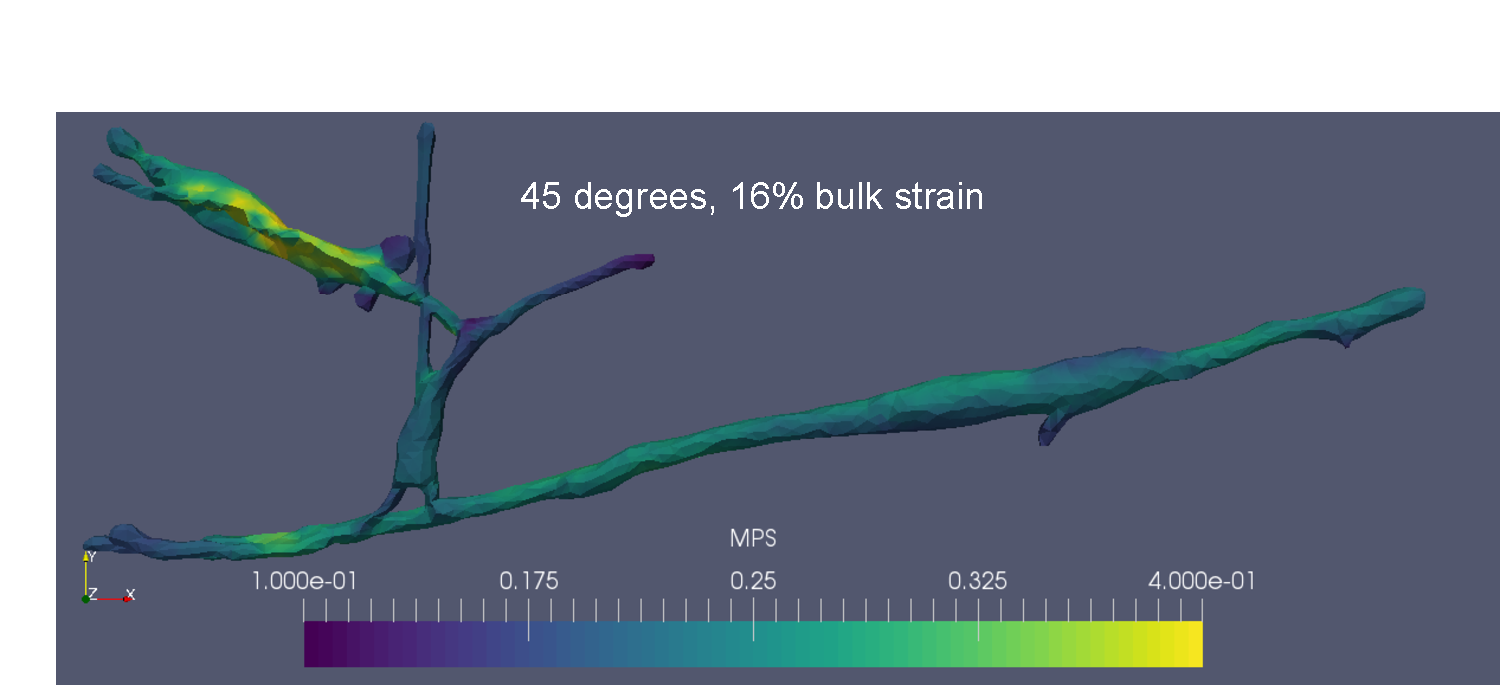
\includegraphics[width=8cm]{figure/MPS_rot45_strain16.pdf} \\
(c) & (d) \\
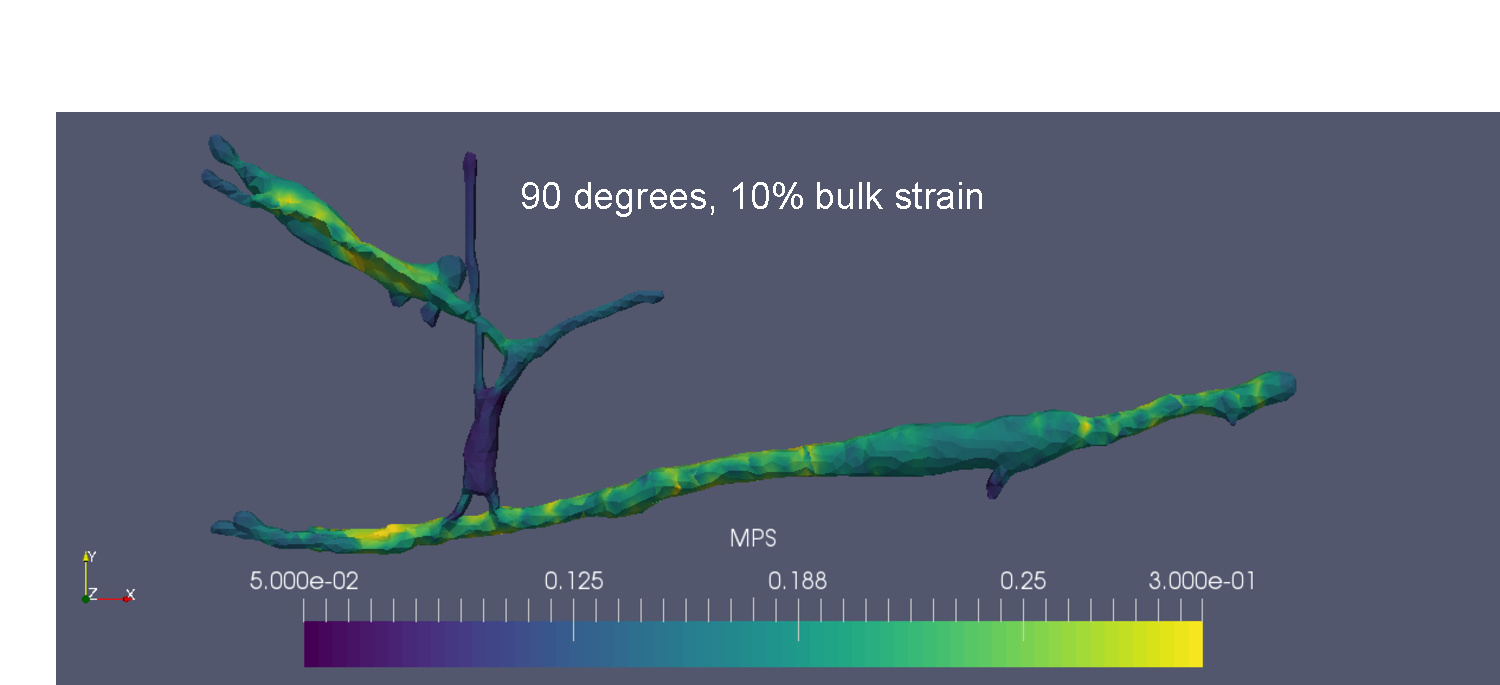
\includegraphics[width=8cm]{figure/MPS_rot90_strain10.pdf} & 
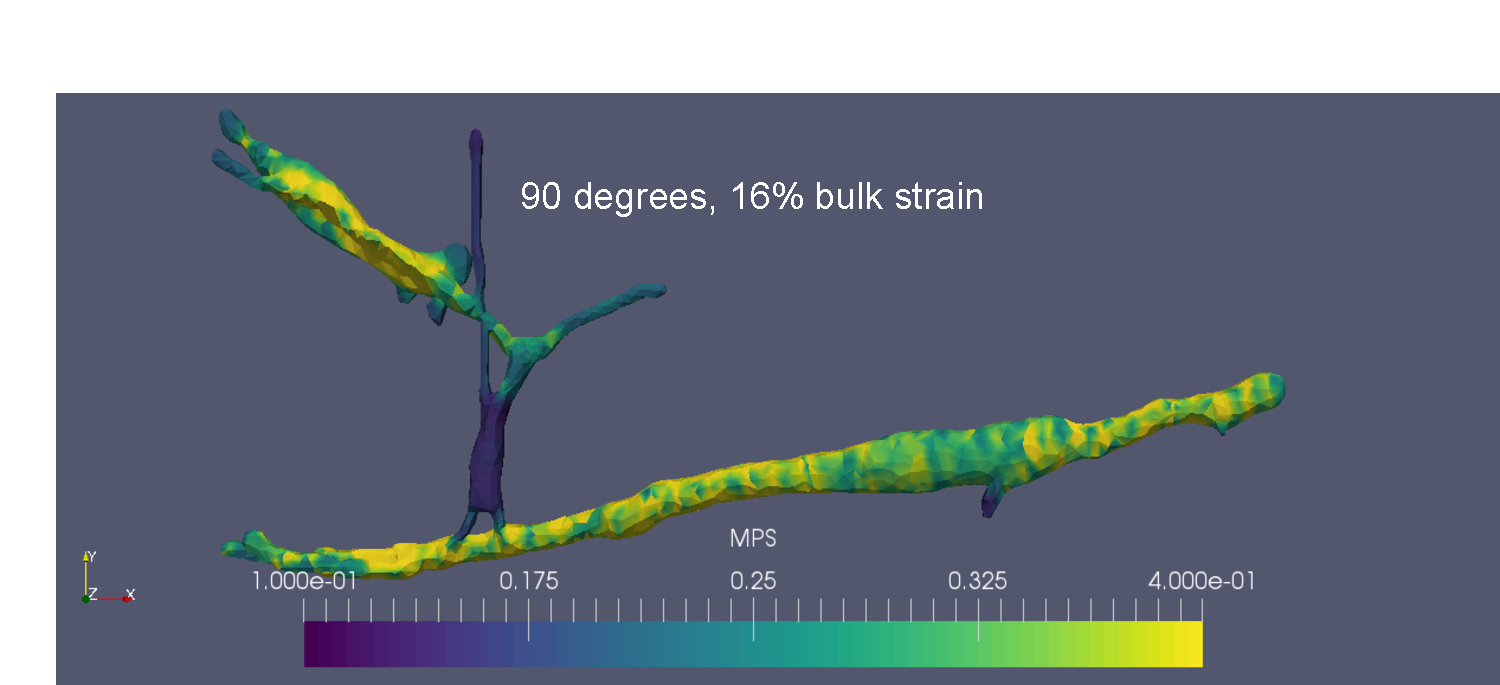
\includegraphics[width=8cm]{figure/MPS_rot90_strain16.pdf} \\
(e) & (f)
\end{array}
$
\end{center}
\caption{\label{fig:neuron_MPS} Color maps of maximum principal strain plotted on neuron structure for loading angles of 0 degrees (first row), 45 degrees (second row), and 90 degrees (third row). Bulk strains of 10$\%$ and 16$\%$ are considered. Note that the color bar ranges from 5$\%$ to 30$\%$ strain for bulk strain of 10$\%$ and from 10$\%$ to 40$\%$ for 16$\%$ bulk strain.}
\end{figure}
%
As seen in Fig.\ \ref{fig:neuron_MPS}, the deformation state varies significantly for different loading angles. In all scenarios, large portions of the neuron experience strains that are greater than the bulk strain that applied to the surrounding gel. This suggests that neurons can be damaged even when the surrounding tissue is loaded moderately. To gain a more quantitative understanding of the amplification of local strains in the neuron, distributions of the maximum principal strain for the neuron are plotted in Fig.\ \ref{fig:neuron_ccdf_mps} for the different loading angles.
%
%0 and 45 degree distributions from N2P178/4-Neuron_FT_trcBC/MaxPrnStrn/PrincipalStrainDistr.m
%90 degree distribution from N2P178/3-Neuron_FT/MaxPrnStrn/PrincipalStrainDistr_FarField.m
\begin{figure}[ht]
\begin{center}
$
\begin{array}{ccc}
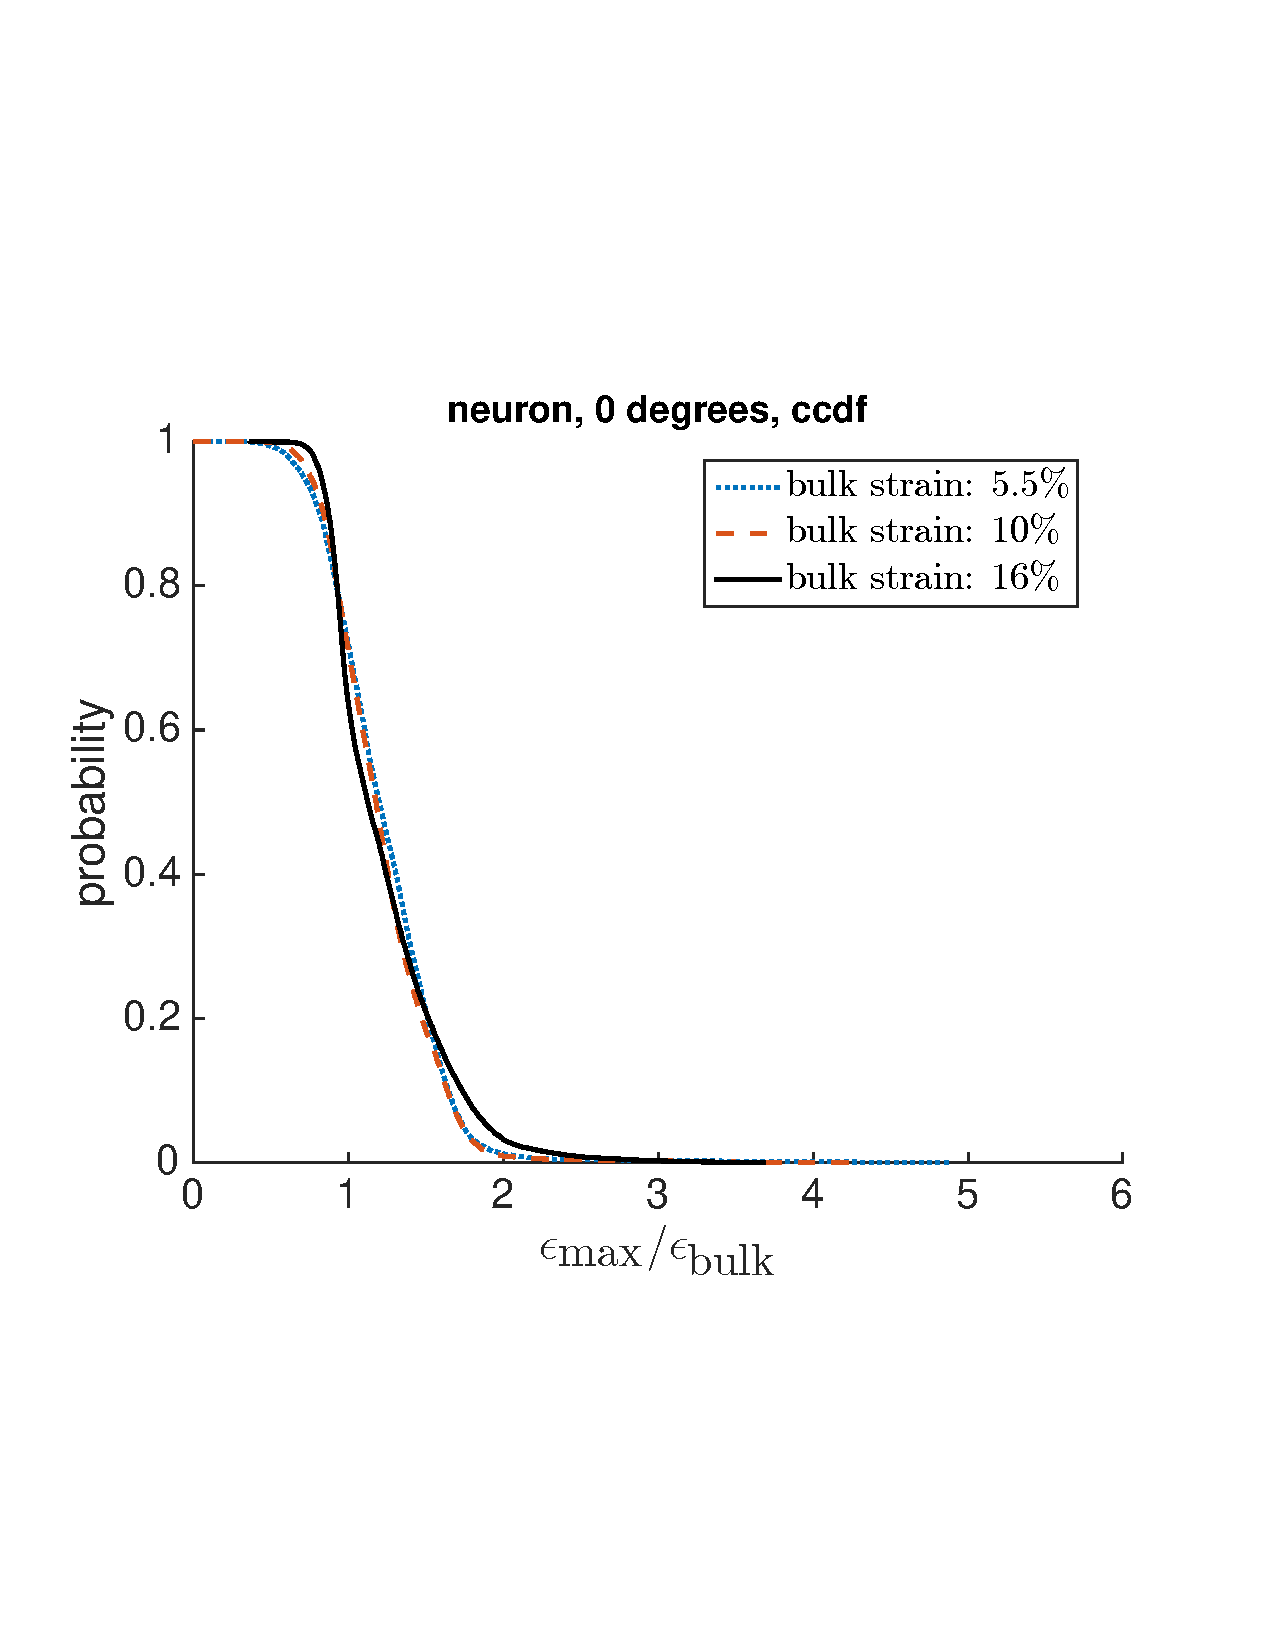
\includegraphics[height=4.5cm]{figure/rot0_FT50_128_1920_ccdf_neuron_compare_stps.pdf} &
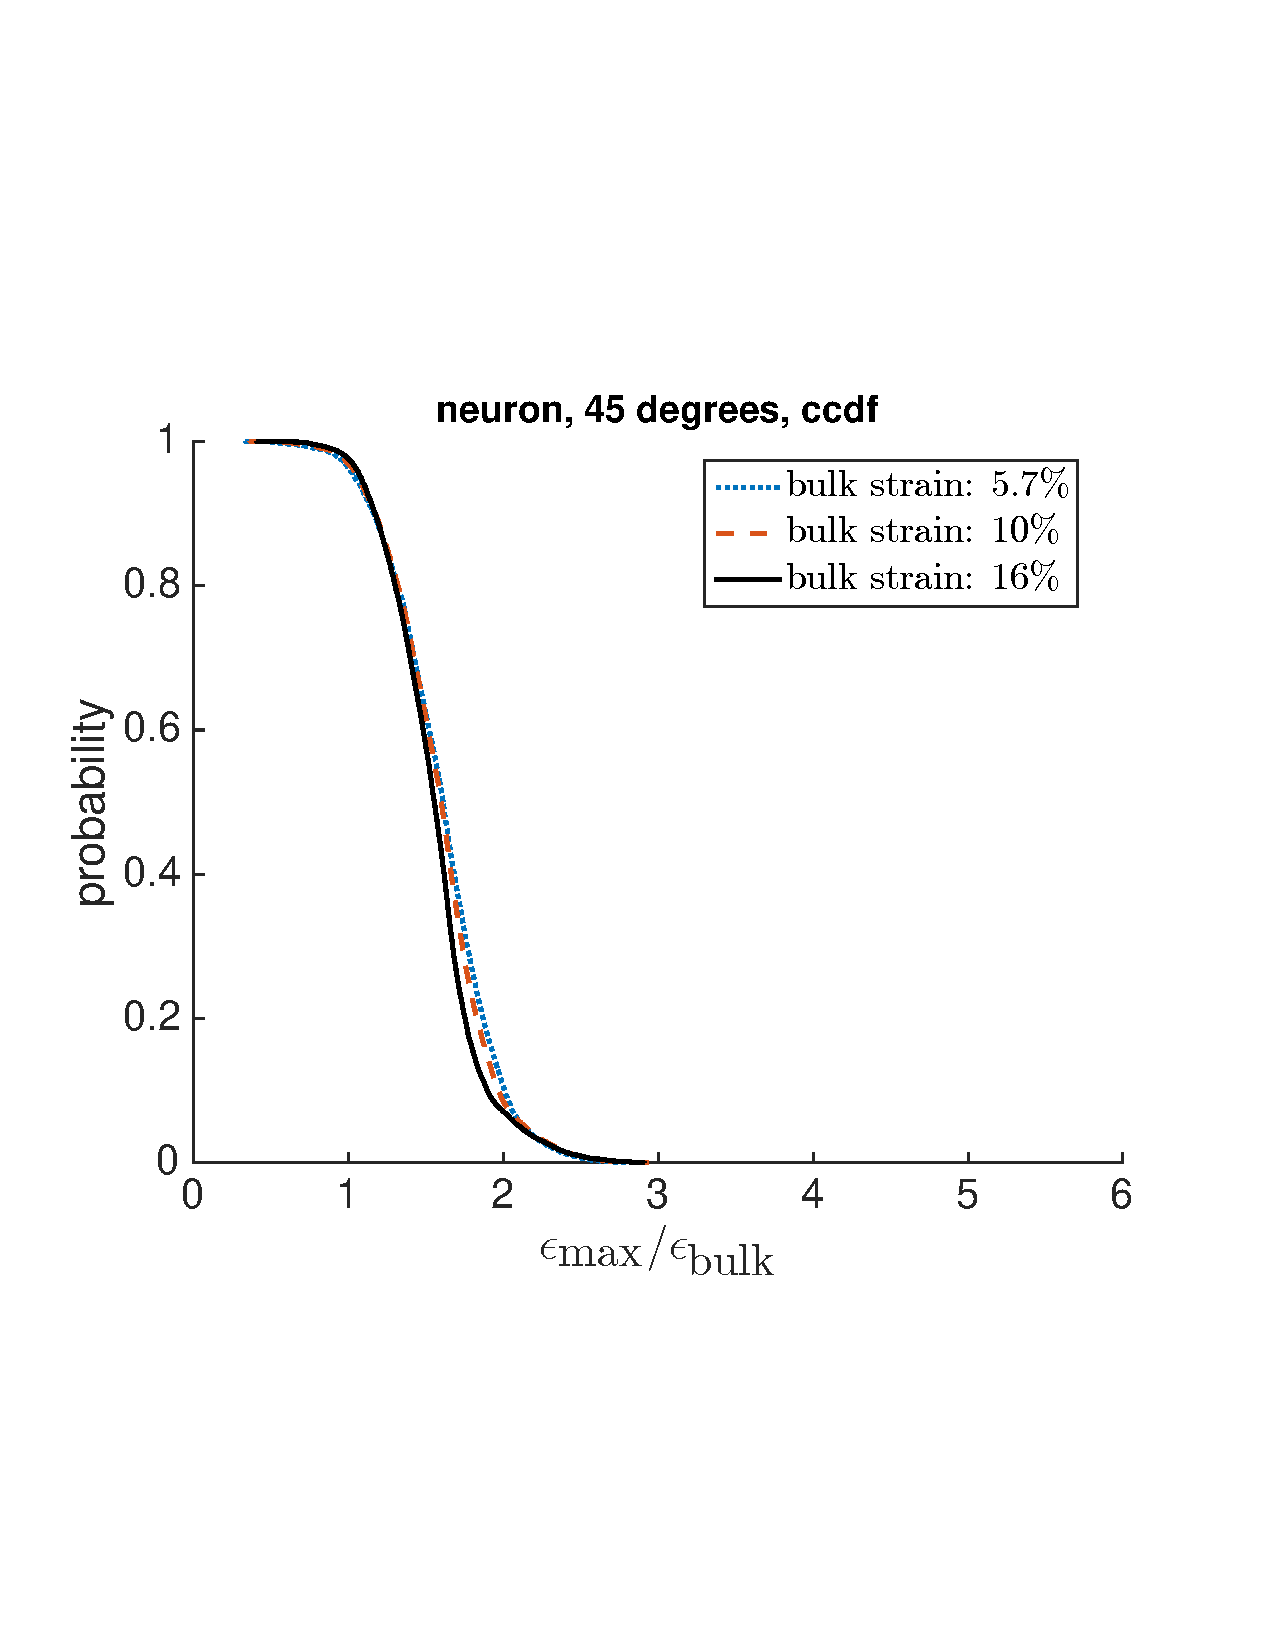
\includegraphics[height=4.5cm]{figure/rot45_FT50_128_1920_ccdf_neuron_compare_stps.pdf} &
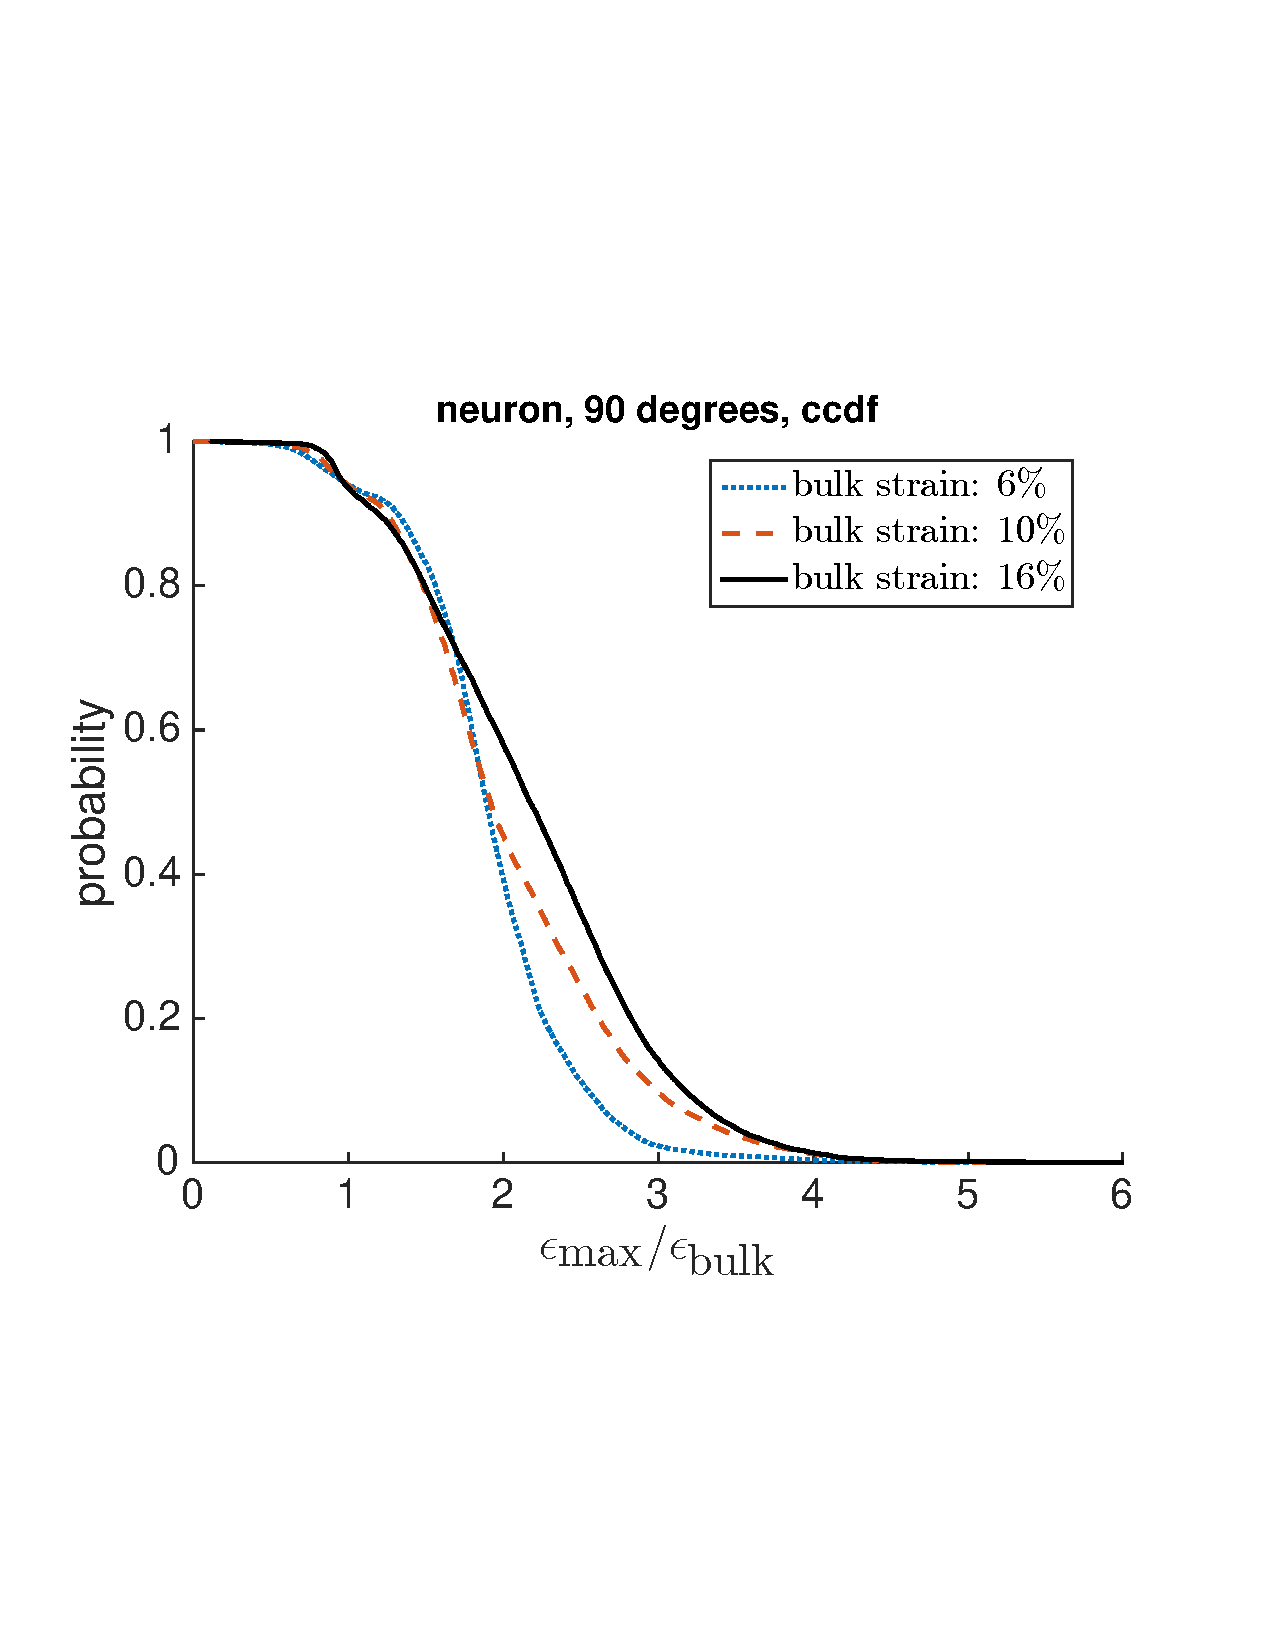
\includegraphics[height=4.5cm]{figure/rot90_FT_dspBC50_a30_128_1920_ccdf_neuron_compare_stps_farfield.pdf} \\
(a) & (b) & (c)
\end{array}
$
\end{center}
\caption{\label{fig:neuron_ccdf_mps} Distributions of maximum principal strain (ccdf) in neuron for loading angles of (a) 0 degrees, (b) 45 degrees, and (c) 90 degrees. For each loading angle, distributions for bulk strains of 5 - 6 $\%$ (dotted blue line), 10$\%$ (dashed red line), and 16$\%$ (solid black line) are plotted. The values of $\epsilon_{\text{max}}$ are normalized by the bulk strain, $\epsilon_{\text{bulk}}$.  }
\end{figure}
%

Consistent with the color maps seen in Fig.\ \ref{fig:neuron_MPS}, the tails of the distributions show that the neuron experiences local strains that are significantly larger than the applied load on the surrounding collagen gel for all loading directions. The amplification in local strain is at least 3 times that of the applied load in the most mild case of 45 degree loading and reaches an amplification of 6 times in the most severe case of the 90 degree loading.

Variation in the shape and spread of the neuron strain distributions at different bulk strains is greatest in the case of 90 degree loading, where the spread of the distributions increase with larger bulk strain. In contrast, the variations in shape and spread of the neuron strain distributions are small for the 0 and 45 degree loading cases. Additional insight can be gained by separating the neuron strain distribution into contributions from the cell bodies and axons. The distributions of maximum principal strain in the cell bodies and axons are plotted in Fig.\ \ref{fig:rgns_ccdf_mps}.
%
\begin{figure}[ht]
\begin{center}
$
\begin{array}{ccc}
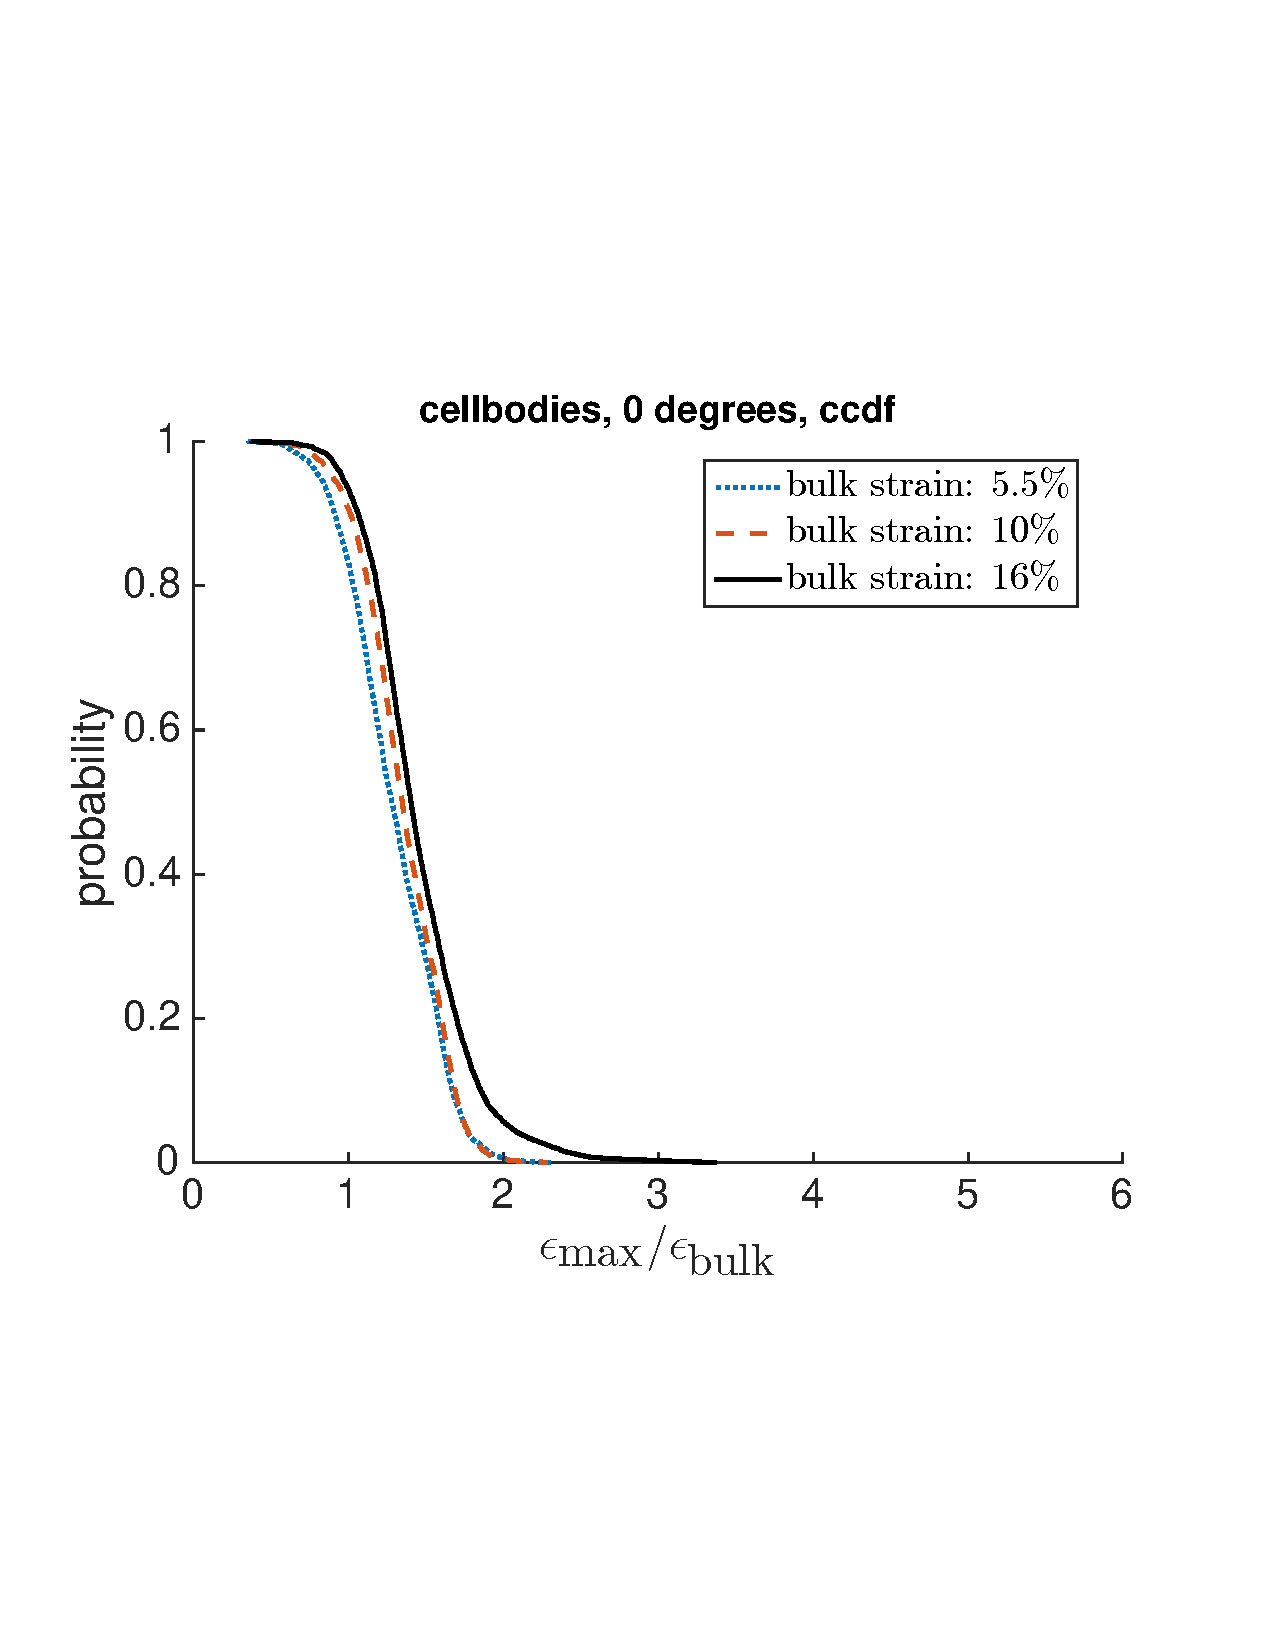
\includegraphics[height=4.5cm]{figure/rot0_FT50_128_1920_ccdf_cellbodies_compare_stps.pdf} & 
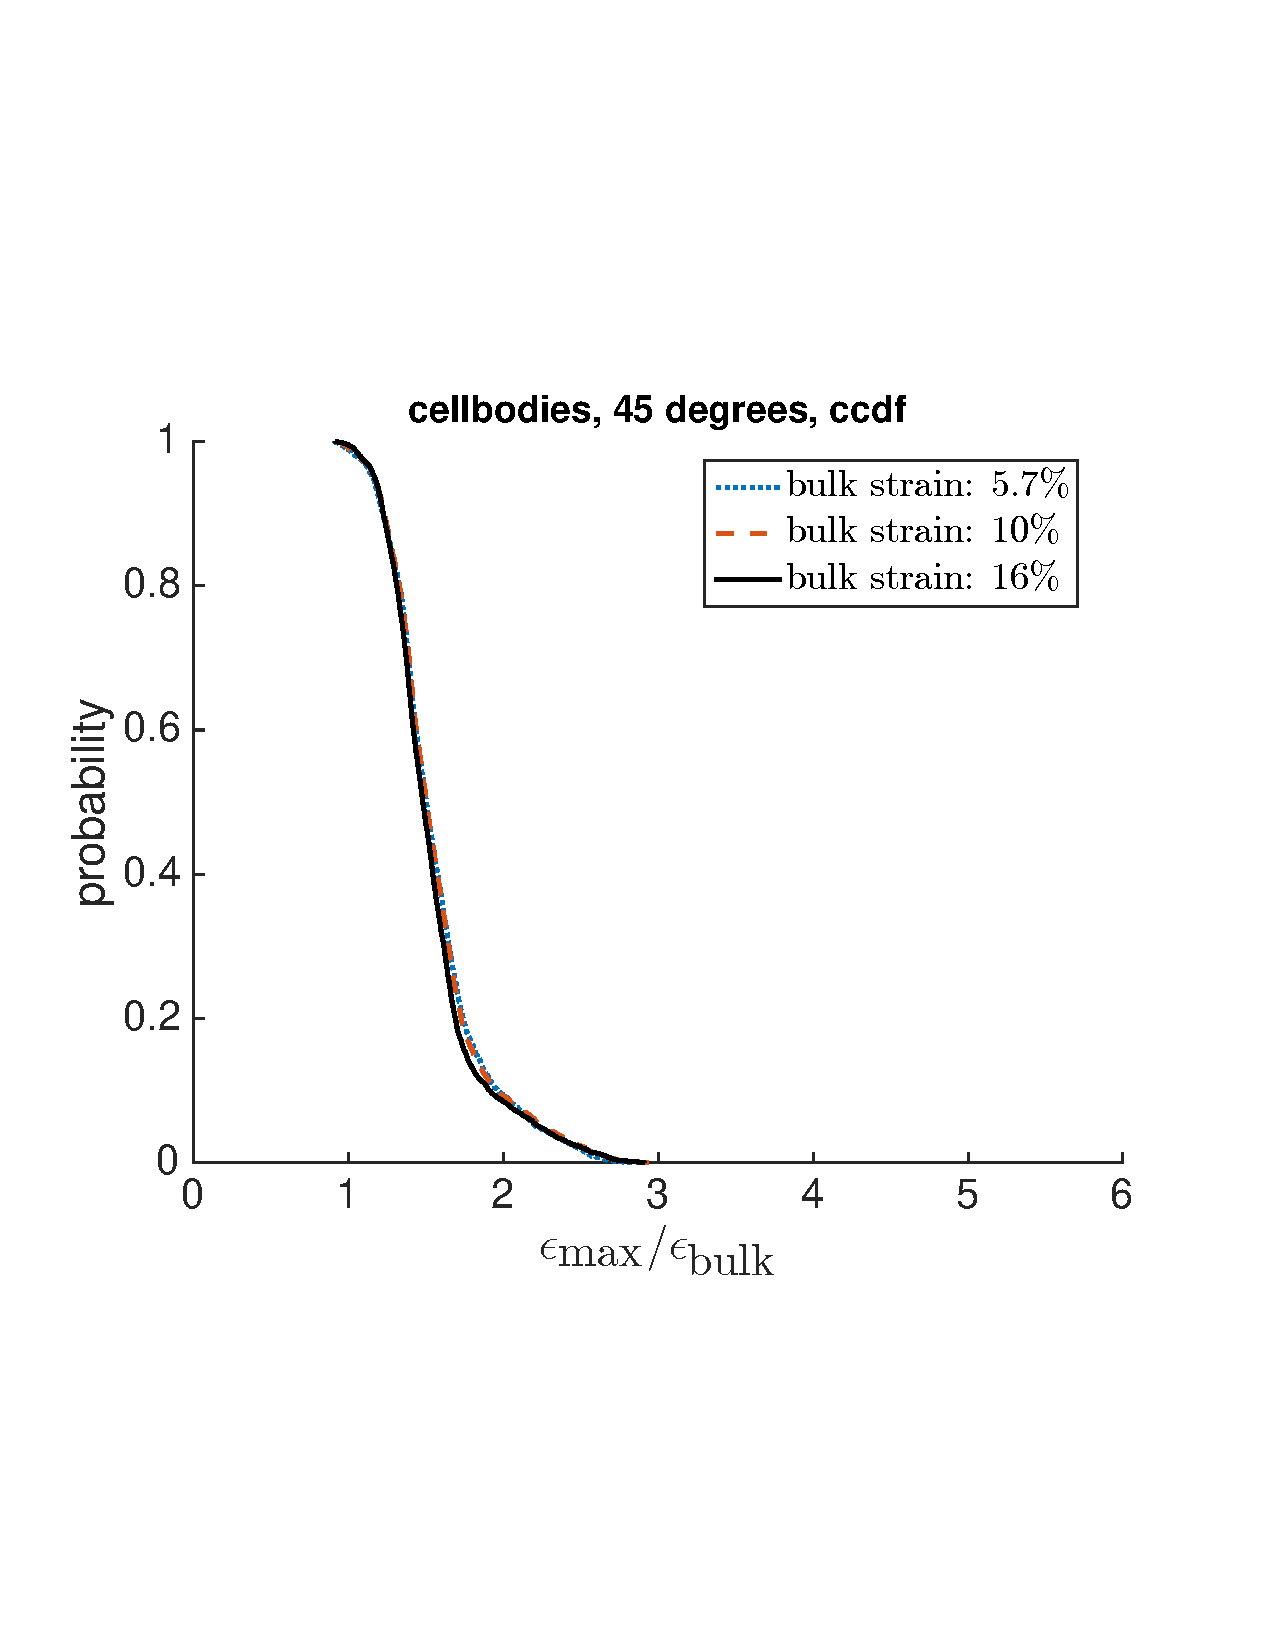
\includegraphics[height=4.5cm]{figure/rot45_FT50_128_1920_ccdf_cellbodies_compare_stps.pdf} & 
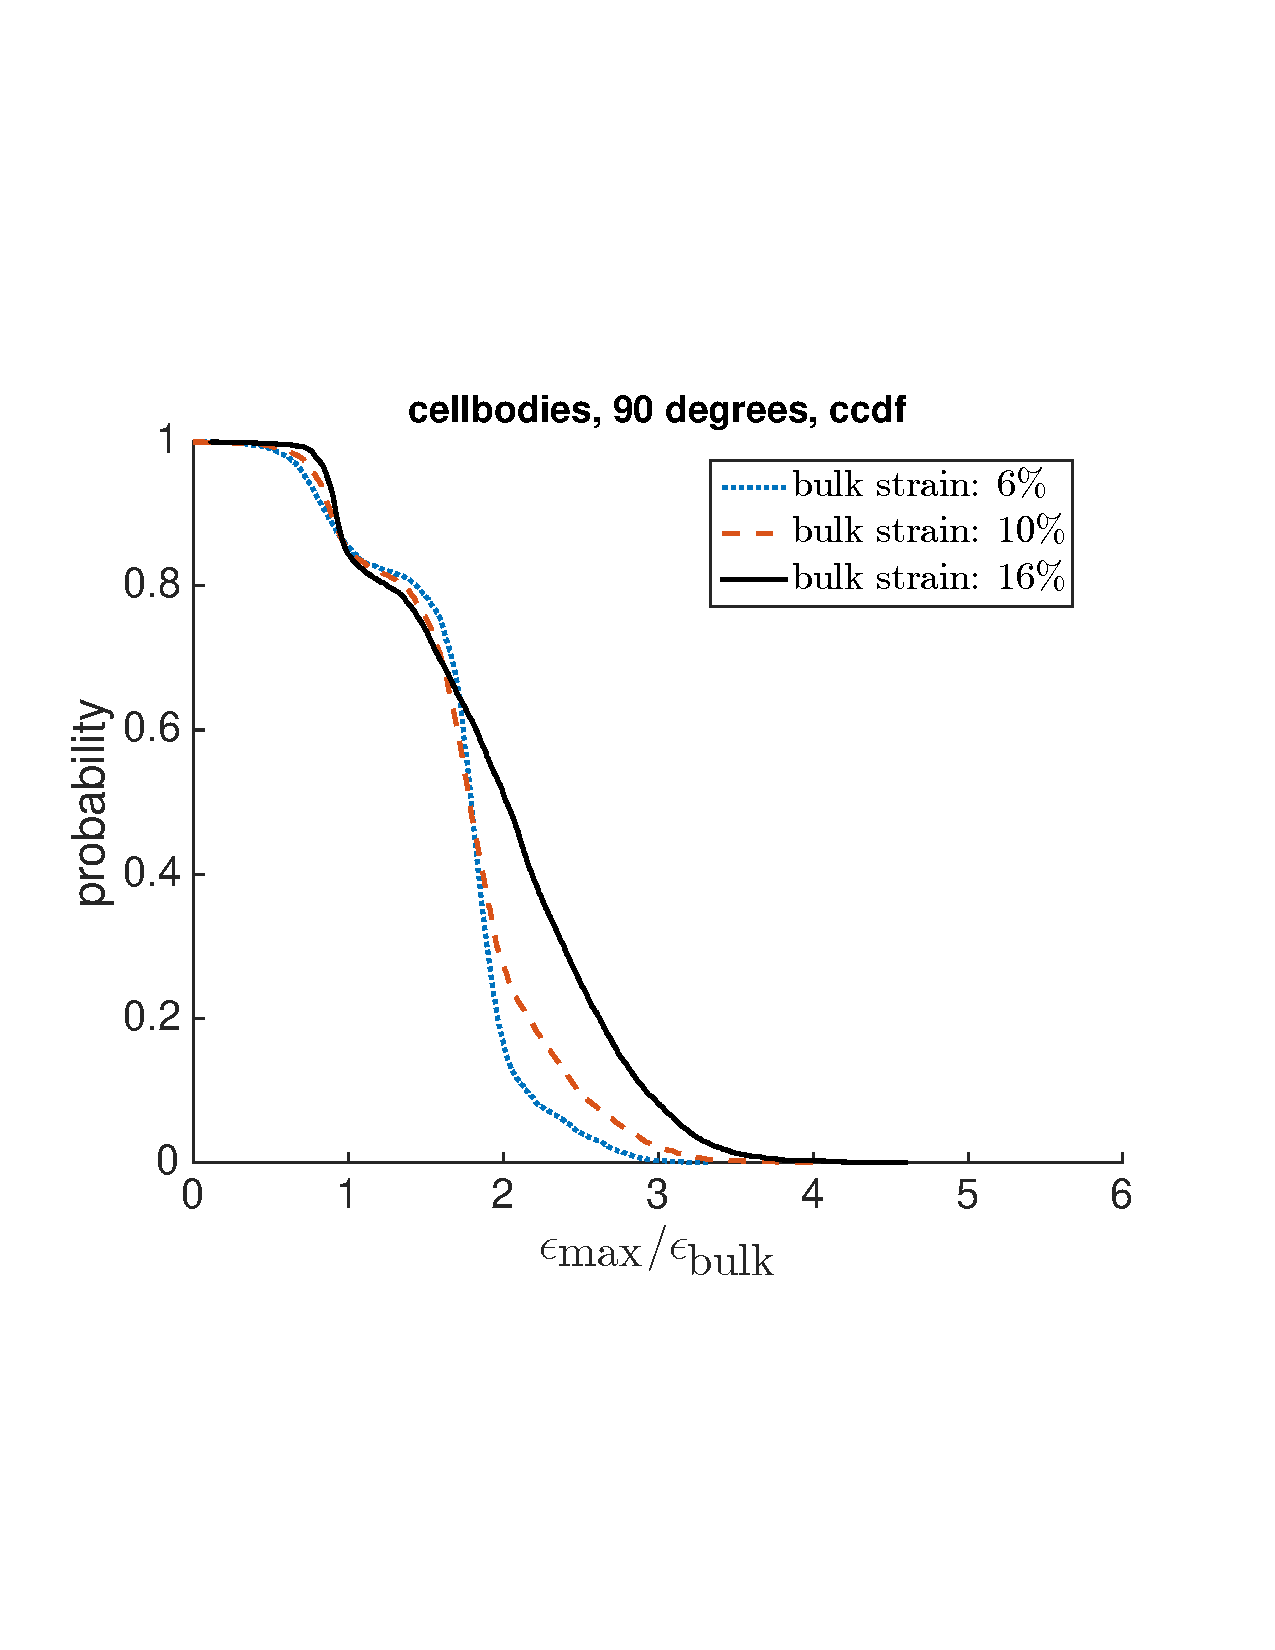
\includegraphics[height=4.5cm]{figure/rot90_FT_dspBC50_a30_128_1920_ccdf_cellbodies_compare_stps_farfield.pdf} \\
(a) & (b) & (c) \\
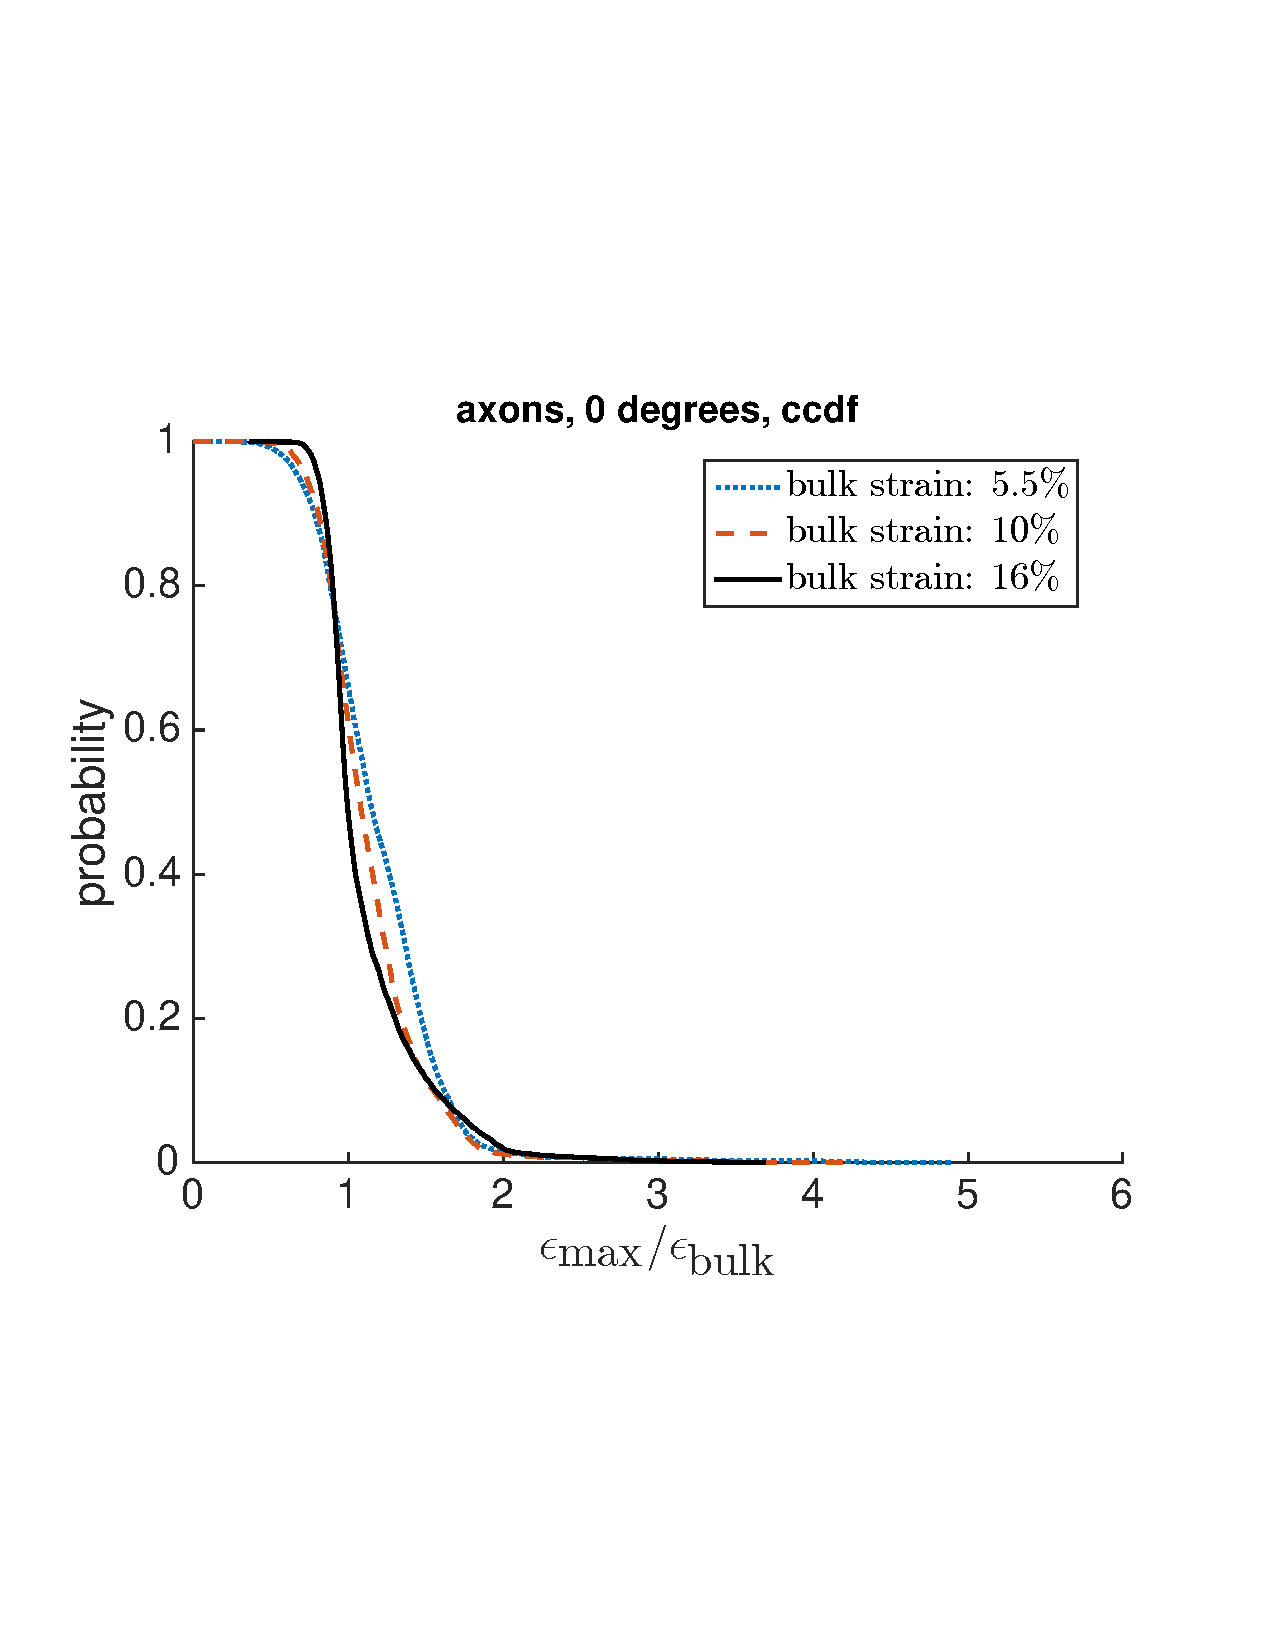
\includegraphics[height=4.5cm]{figure/rot0_FT50_128_1920_ccdf_axons_compare_stps.pdf} &
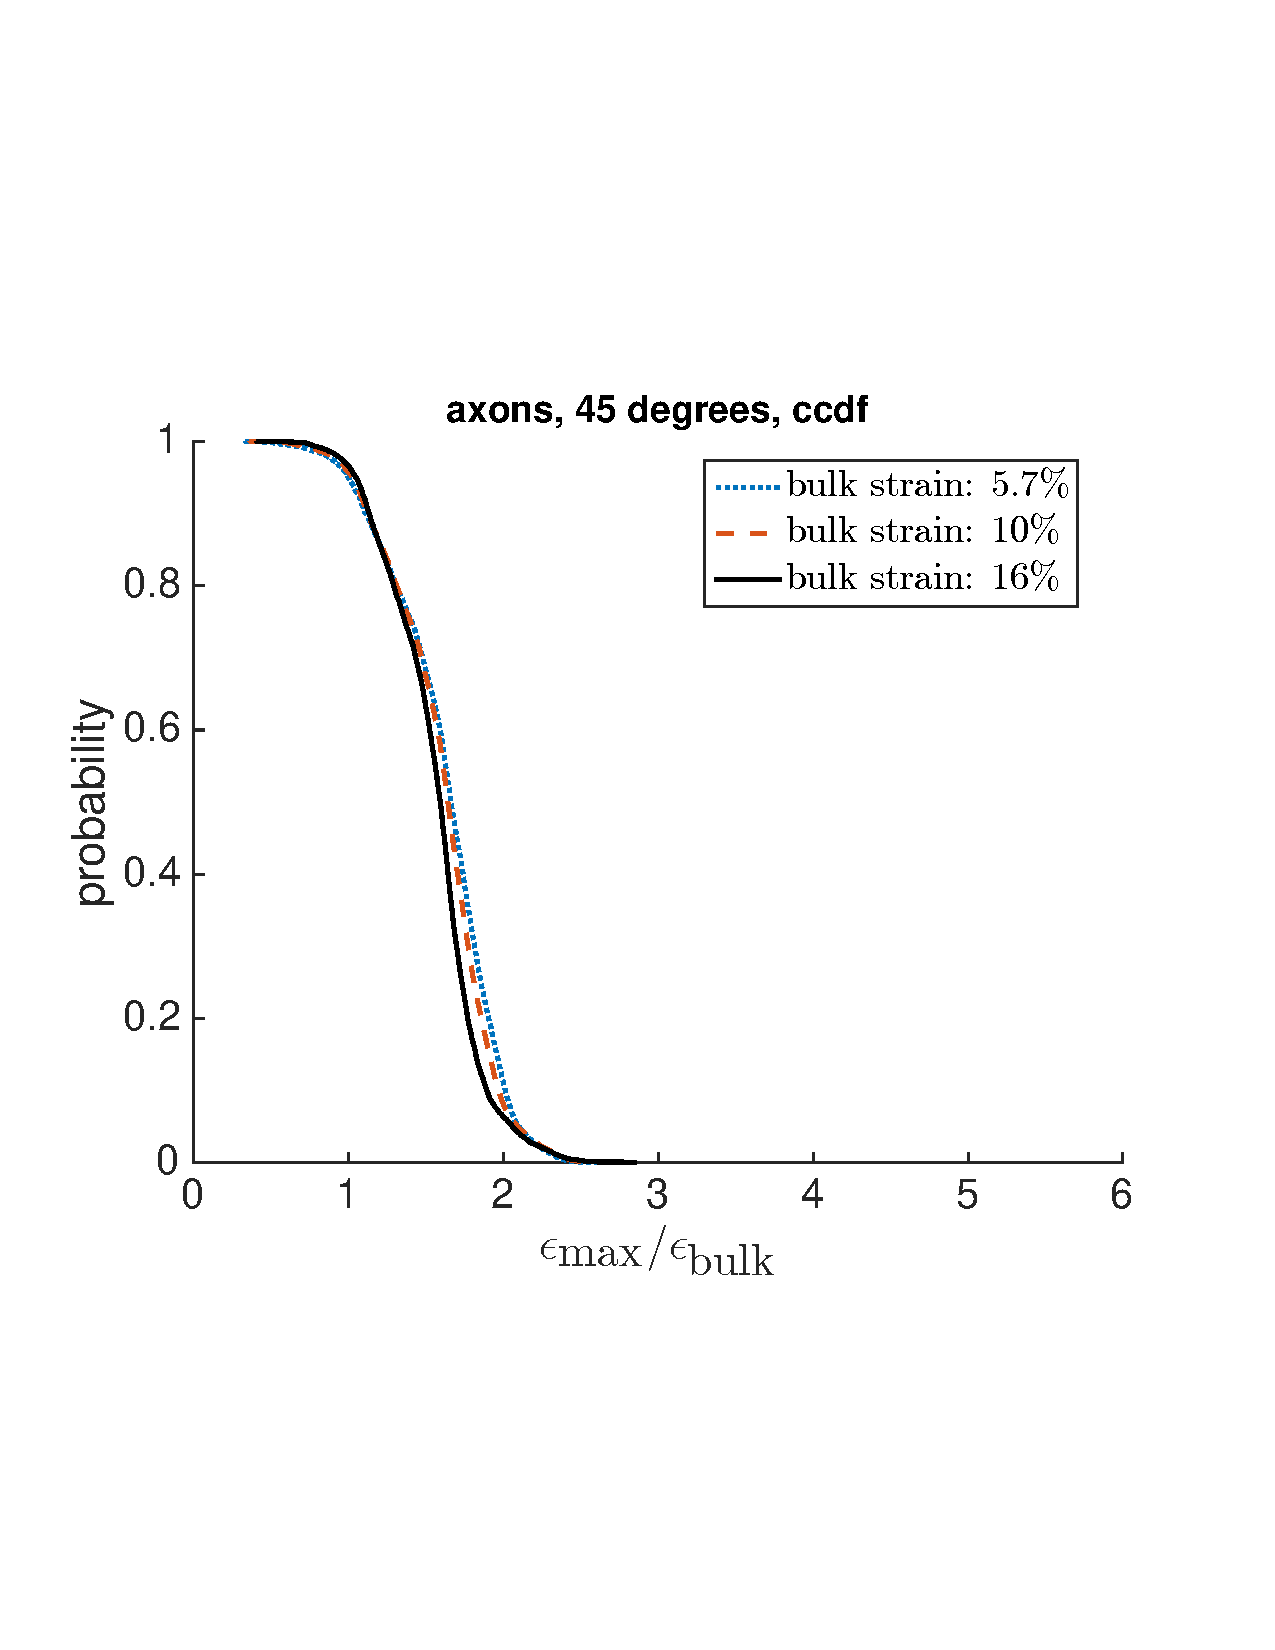
\includegraphics[height=4.5cm]{figure/rot45_FT50_128_1920_ccdf_axons_compare_stps.pdf} &
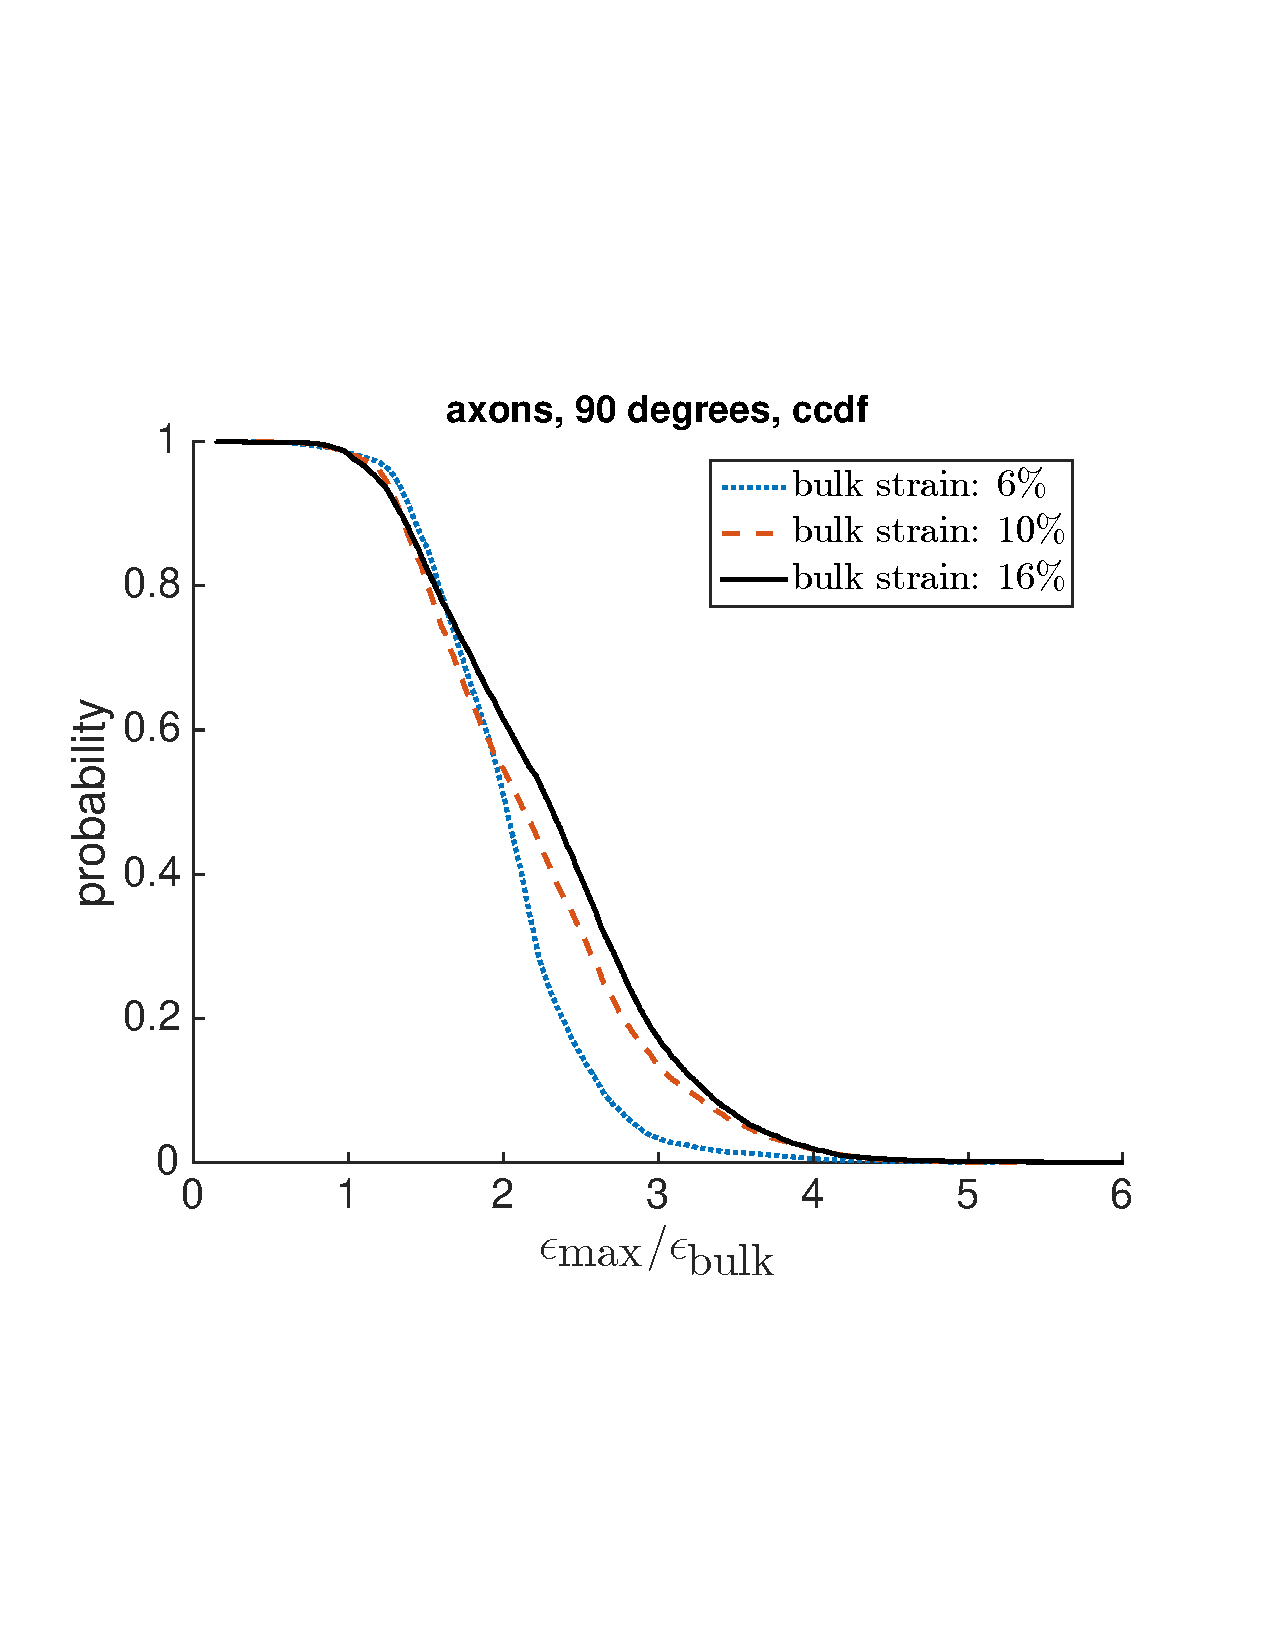
\includegraphics[height=4.5cm]{figure/rot90_FT_dspBC50_a30_128_1920_ccdf_axons_compare_stps_farfield.pdf} \\
(d) & (e) & (f)
\end{array}
$
\end{center}
\caption{\label{fig:rgns_ccdf_mps} Distributions of maximum principal strain (ccdf) in the cell bodies (top row) and axons (bottom row) for loading angles of (a,d) 0 degrees, (b,e) 45 degrees, and (c,f) 90 degrees. For each loading angle, distributions for bulk strains of 5 - 6 $\%$ (dotted blue line), 10$\%$ (dashed red line), and 16$\%$ (solid black line) are plotted. The values of $\epsilon_{\text{max}}$ are normalized by the bulk strain, $\epsilon_{\text{bulk}}$.  }
\end{figure}
%

The separate distributions for the cell bodies and axons provide additional details about the variations in shape and spread of the neuron distributions in Fig.\ \ref{fig:neuron_ccdf_mps}. For the 0 degree loading case, variations in the distribution at different bulk strains become more apparent. For the cell bodies, the distribution shifts to the right for larger bulk strains indicating that the amplification in the local strain becomes larger with more deformation in the surrounding gel. On the contrary, the middle portion of the axon distribution shifts to the left with increasing bulk strains indicating that the local strain amplification decreases with more deformation in the surrounding gel. The response in the cell bodies and axons cancel out resulting in only slight variations in the overall neuron strain distribution.

For the 45 degree loading case, variations only arise in the axon distribution. Therefore, the variations seen in the overall neuron distribution is solely due to variations in the axon. As in the 0 degree loading case, the axon distribution shifts to the left with larger bulk strains indicating a decrease in the local strain amplification as the surrounding gel is increasingly deformed.

For the 90 degree loading case, large variations are seen in both the cell body and axon distributions. For the cell bodies, the subtle step feature seen in the overall neuron distribution becomes more apparent. This step feature corresponds to two regimes of strain which are clearly seen in the over plot of maximum principal strain on the neuron in Figs.\ \ref{fig:neuron_MPS}(e) and (f). For both the cell body and axon, the distributions shift to the right with increasing bulk strains indicating that the local strain amplification increases with increasing deformation in the surrounding gel. 

The results above indicate that the local strains experienced by the neuron is significantly larger than the applied load on the surrounding gel. The extent of local strain amplification depends on the configuration of the neuron relative to the loading angle. To clarify the cause of local strain amplification in the neuron, the axial strains along a region of the neuron structure are examined.

%=========================================================================================================
\subsection{Axial Strain Distributions}
The axial strains in the region of the neuron highlighted in Fig.\ \ref{fig:axial_schematic} are examined - these axes are also specified in Fig.\ \ref{fig:axial_schematic}. The strain distributions for this region of the neuron are plotted in Fig.\ \ref{fig:axial_mps_distr}. 
%
\begin{figure}[ht]
\begin{center}
$
\begin{array}{c}
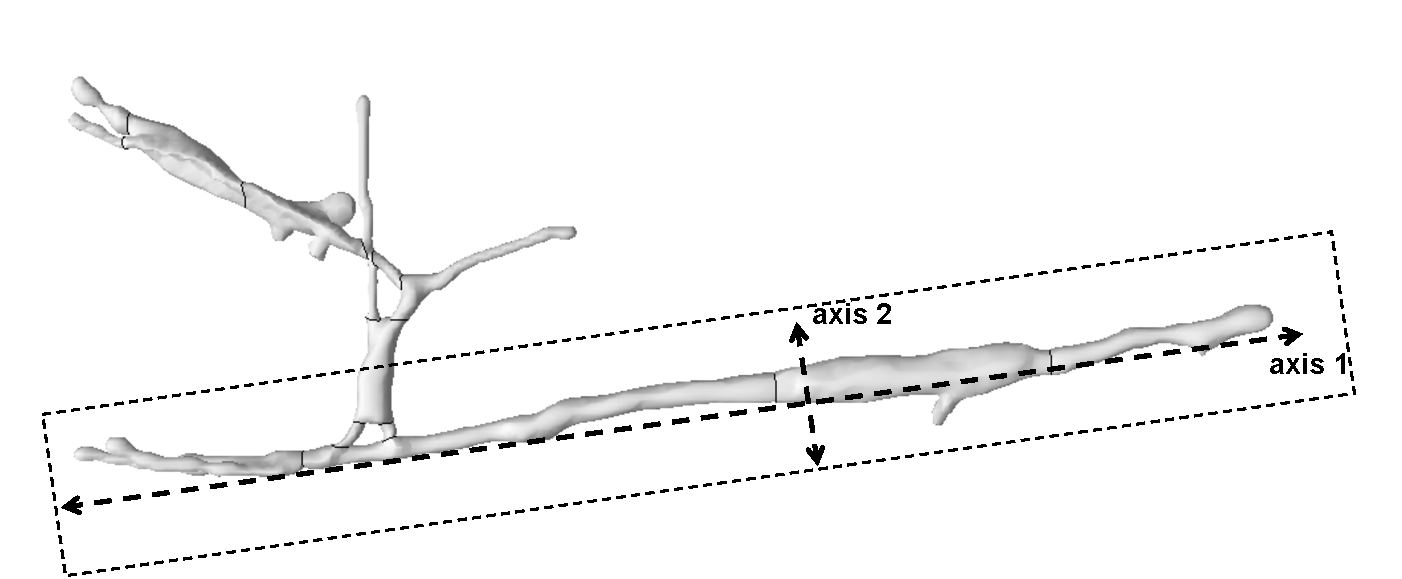
\includegraphics[height=4cm]{figure/axial_coords_schematic.pdf} 
\end{array}
$
\end{center}
\caption{\label{fig:axial_schematic} Schematic showing the region (rectangular box) and the axes (dashed lines) that are examined.}
\end{figure}
%
The three angles of applied load schematically shown in Fig.\ \ref{fig:analysis_schematic} are considered. Depending on the loading angle, axes 1 and 2 will experience either tensile or compressive axial strains. For tensile strains, the complementary cumulative distribution function (ccdf), Eq.\ \eqref{eq:comp_cdf}, is applied so that one can read ``X percent (ordinate) of the structure contains \textit{at least} Y tensile strain (abscissa)" from the distribution plot. On the other hand, for compressive strains, which are negative in value, the cumulative distribution function (cdf) is applied so that one similarly can read ``X percent (ordinate) of the structure contains \textit{at least} (with respect to magnitude) Y compressive strain (abscissa)" from the distribution plot. In the case where load is applied at 0 degrees, axes 1 and 2 experience tensile and compressive axial strains, respectively. Similarly, when load is applied at 45 degrees, axis 1 experiences tensile axial strains while axis 2 experiences mostly compressive axial strains with a small fraction of the structure experiencing tensile strains. On the other hand, when load is applied at 90 degrees, axes 1 and 2 experience compressive and axial strains, respectively.  
%
\begin{figure}[ht]
\begin{center}
$
\begin{array}{ccc}
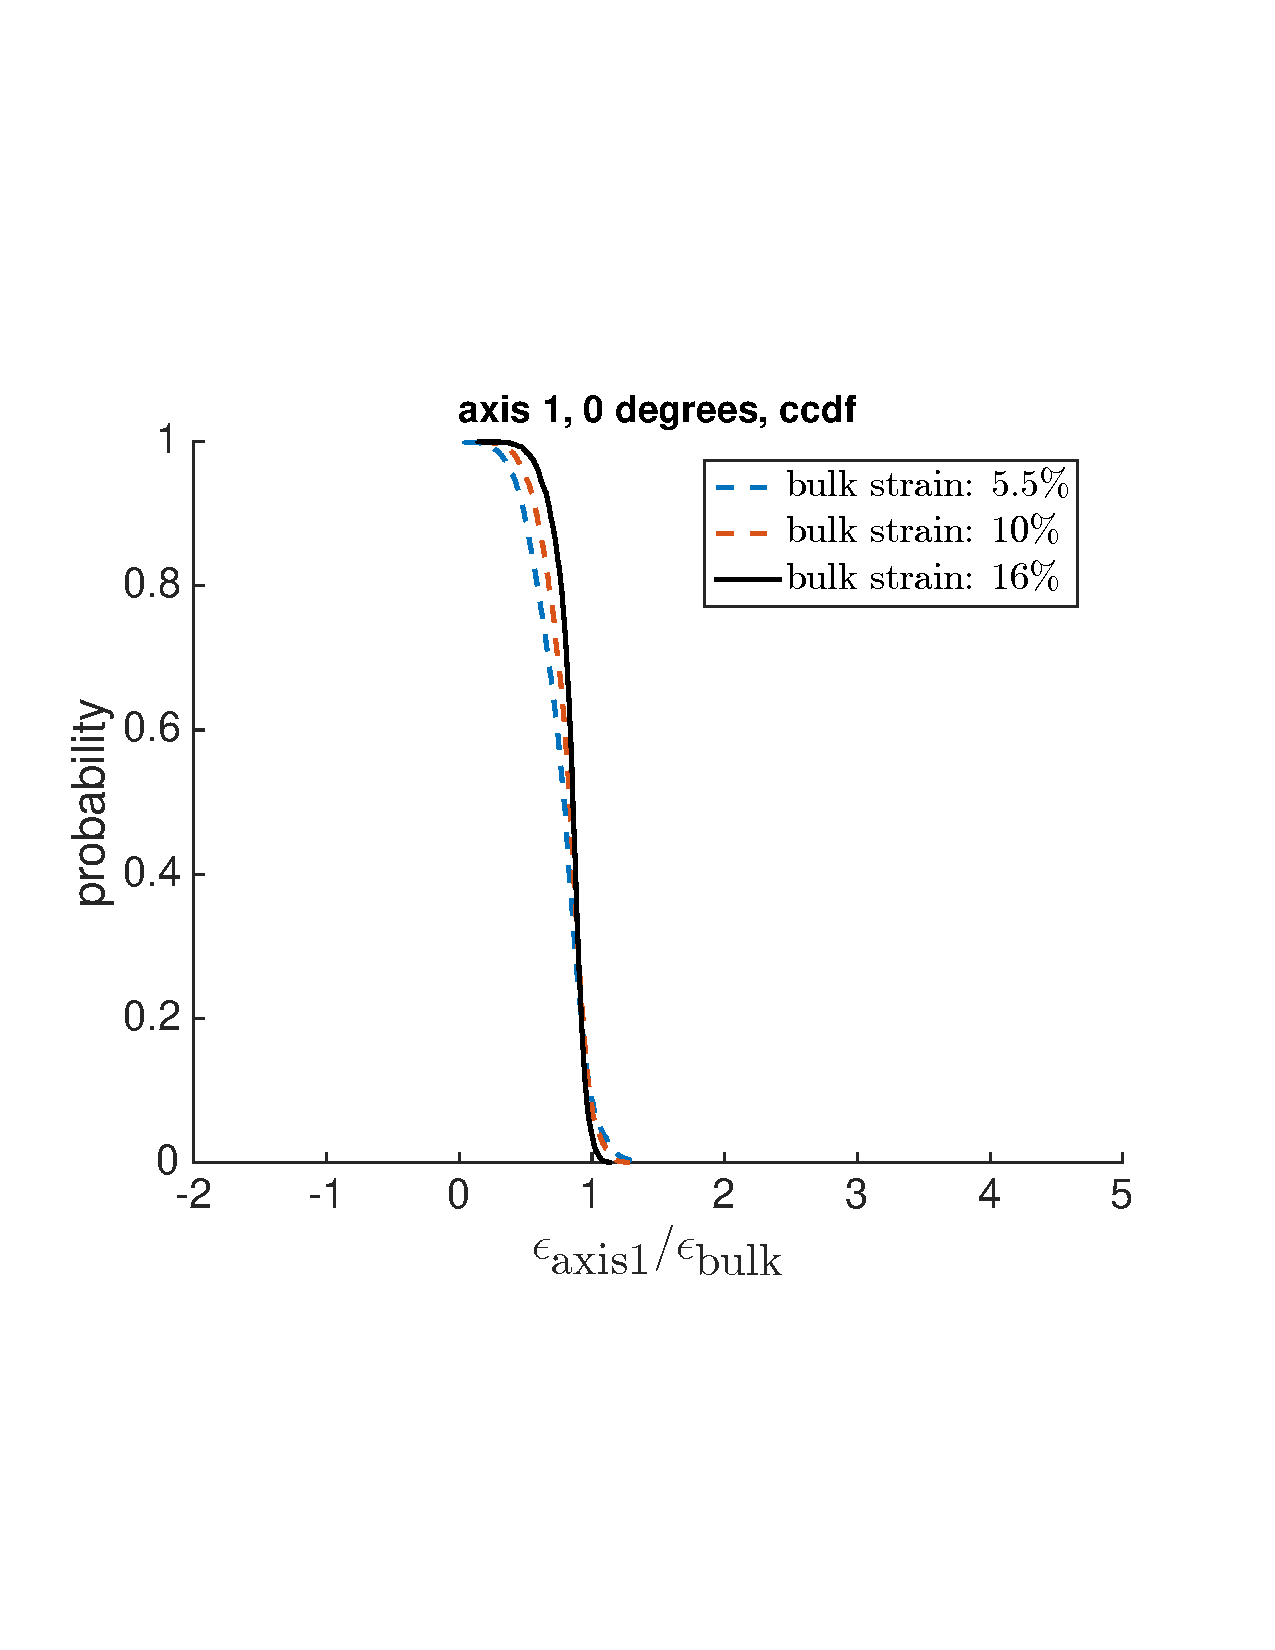
\includegraphics[height=4.5cm]{figure/rot0_FT50_strn11_128_1920_axial_ccdf_axis1_compare_stps.pdf} & 
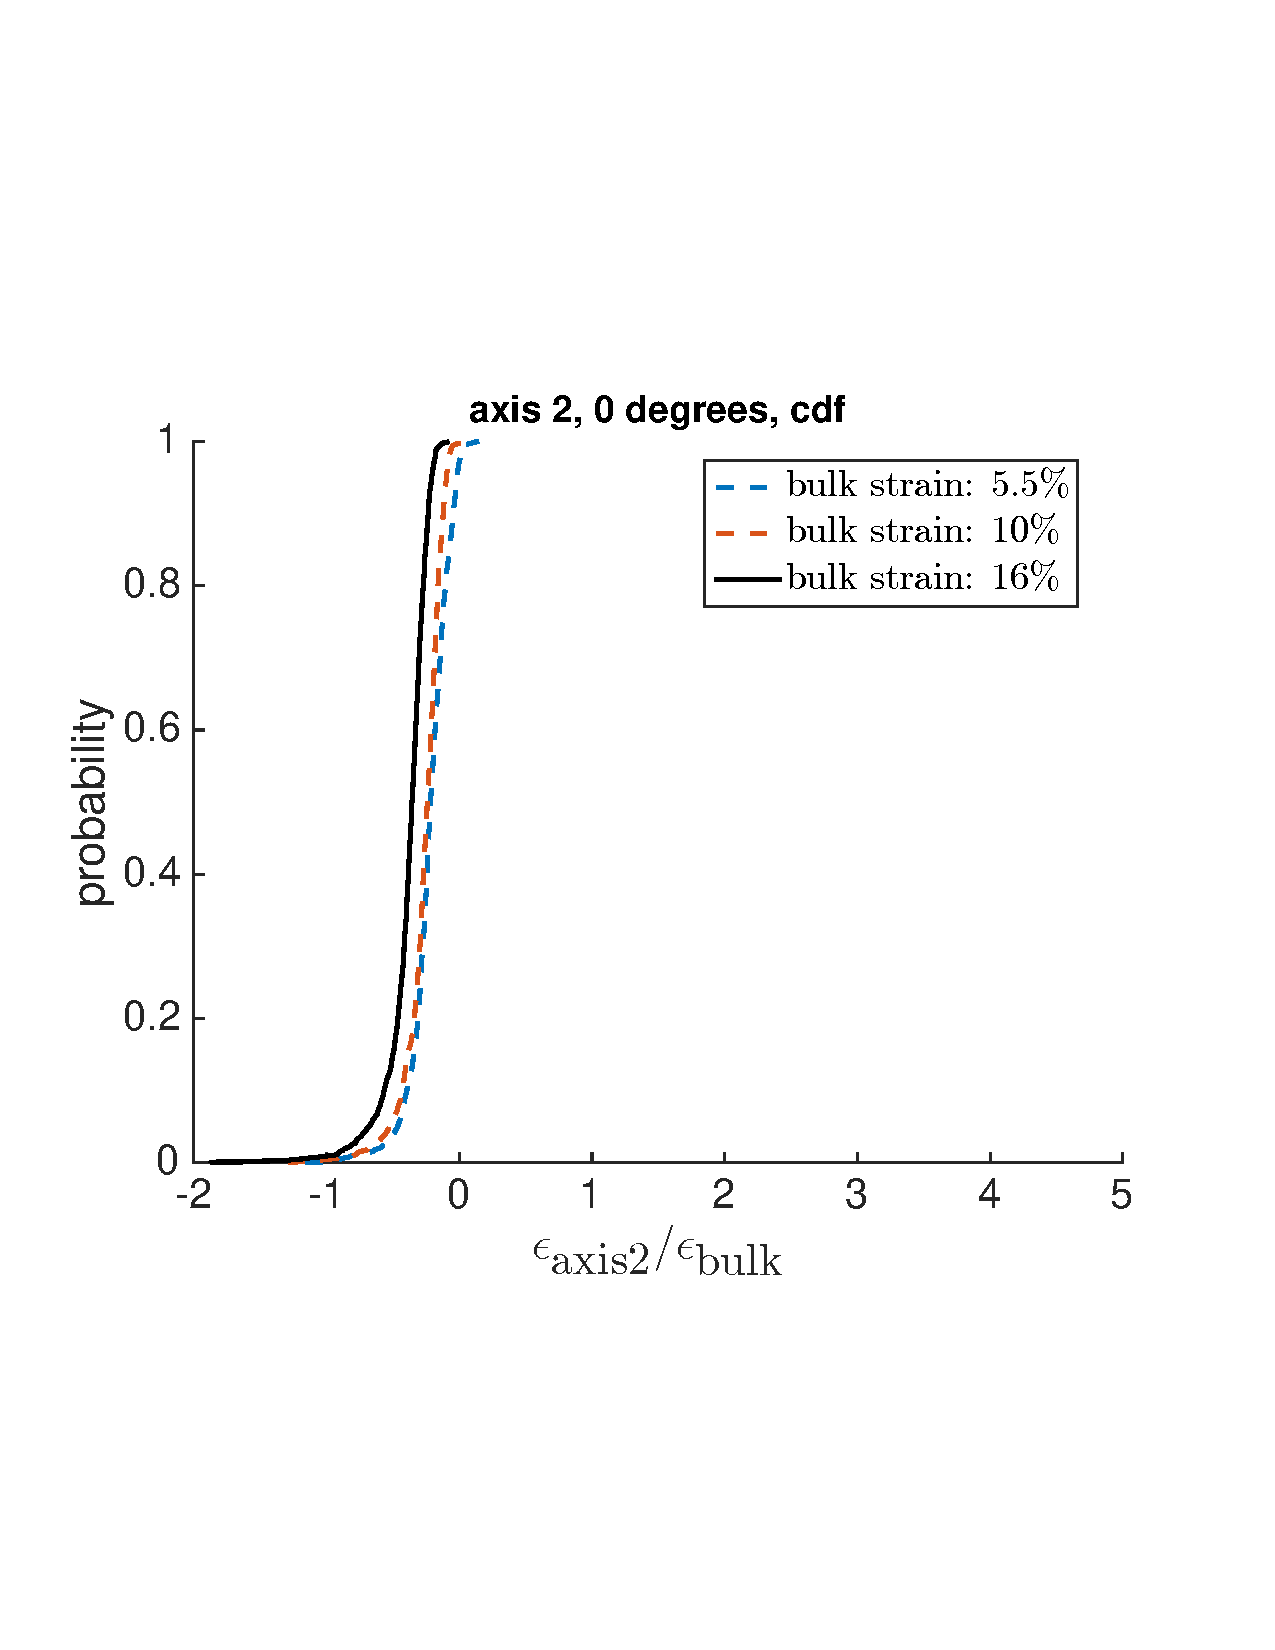
\includegraphics[height=4.5cm]{figure/rot0_FT50_strn22_128_1920_axial_cdf_axis1_compare_stps.pdf} & 
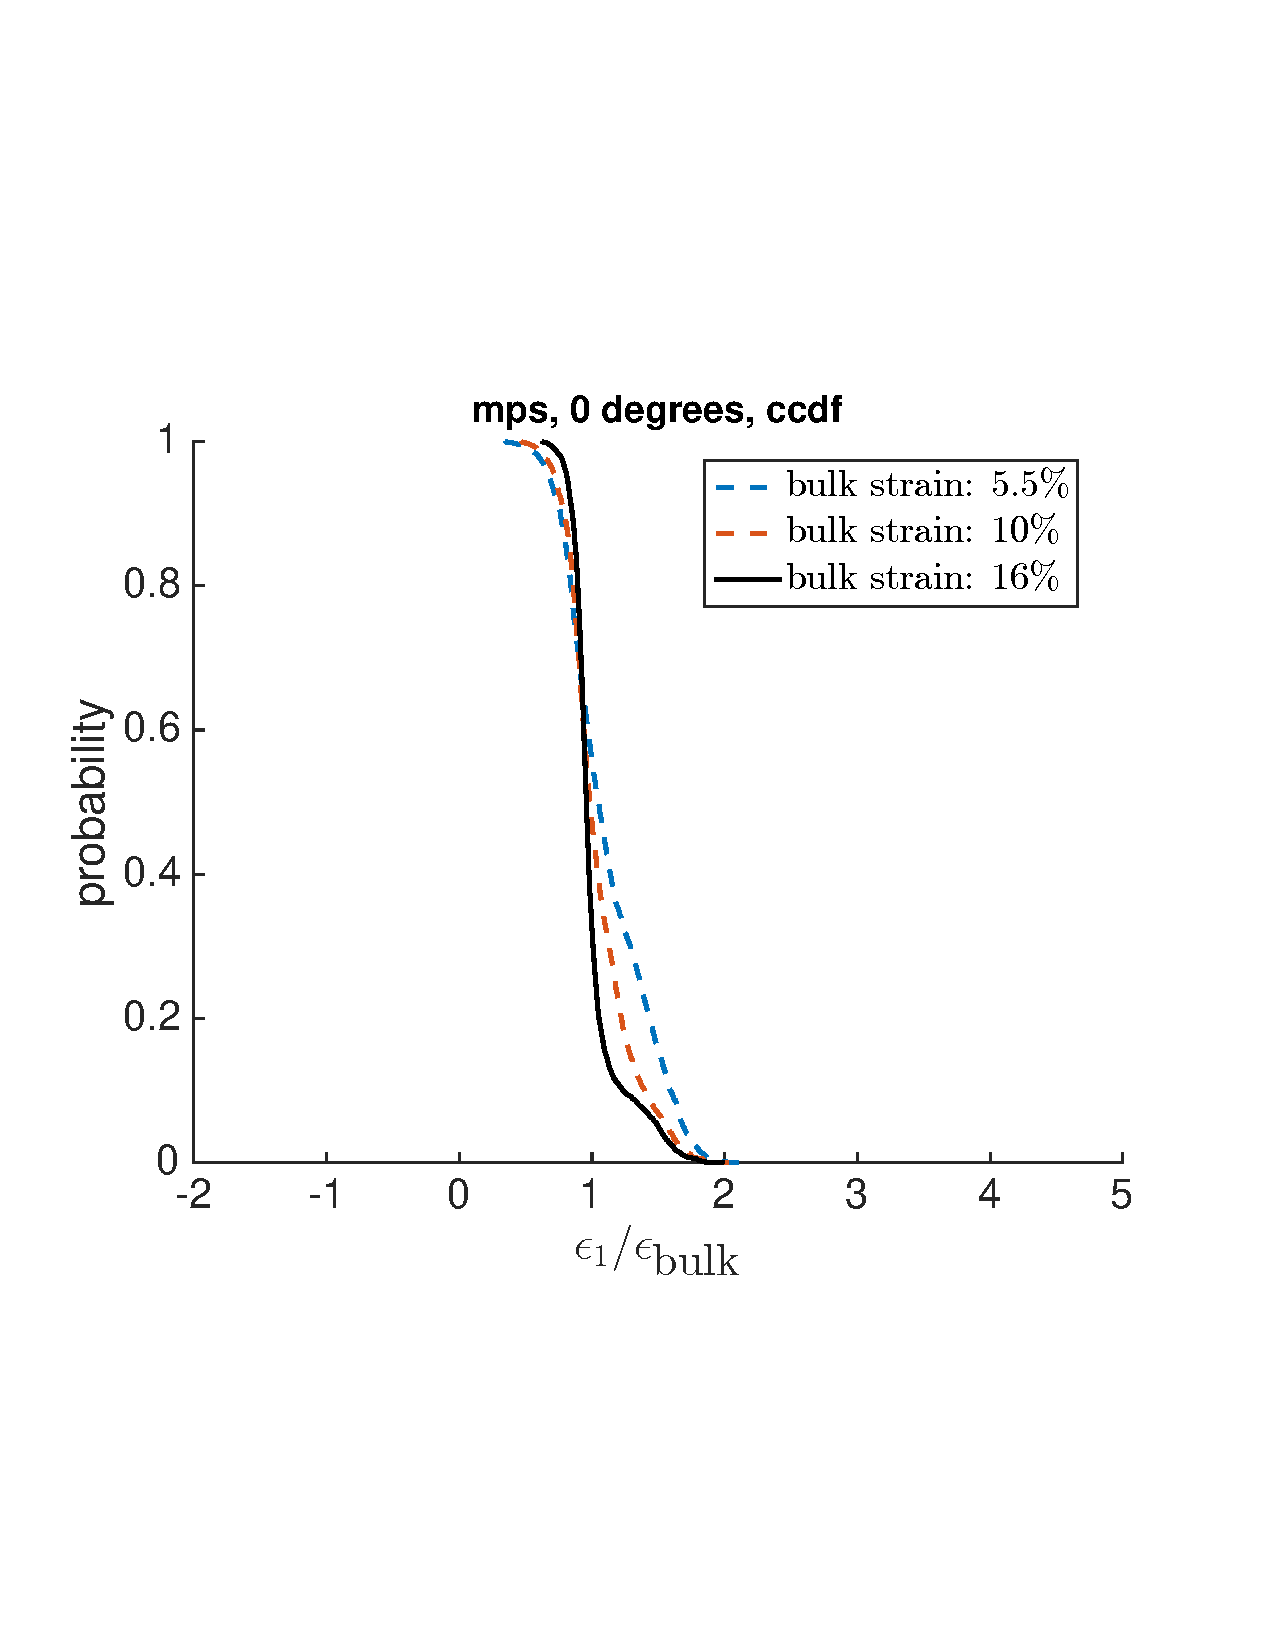
\includegraphics[height=4.5cm]{figure/rot0_FT50_strn11_128_1920_mps_ccdf_axis1_compare_stps.pdf} \\
(a) & (b) & (c) \\ 
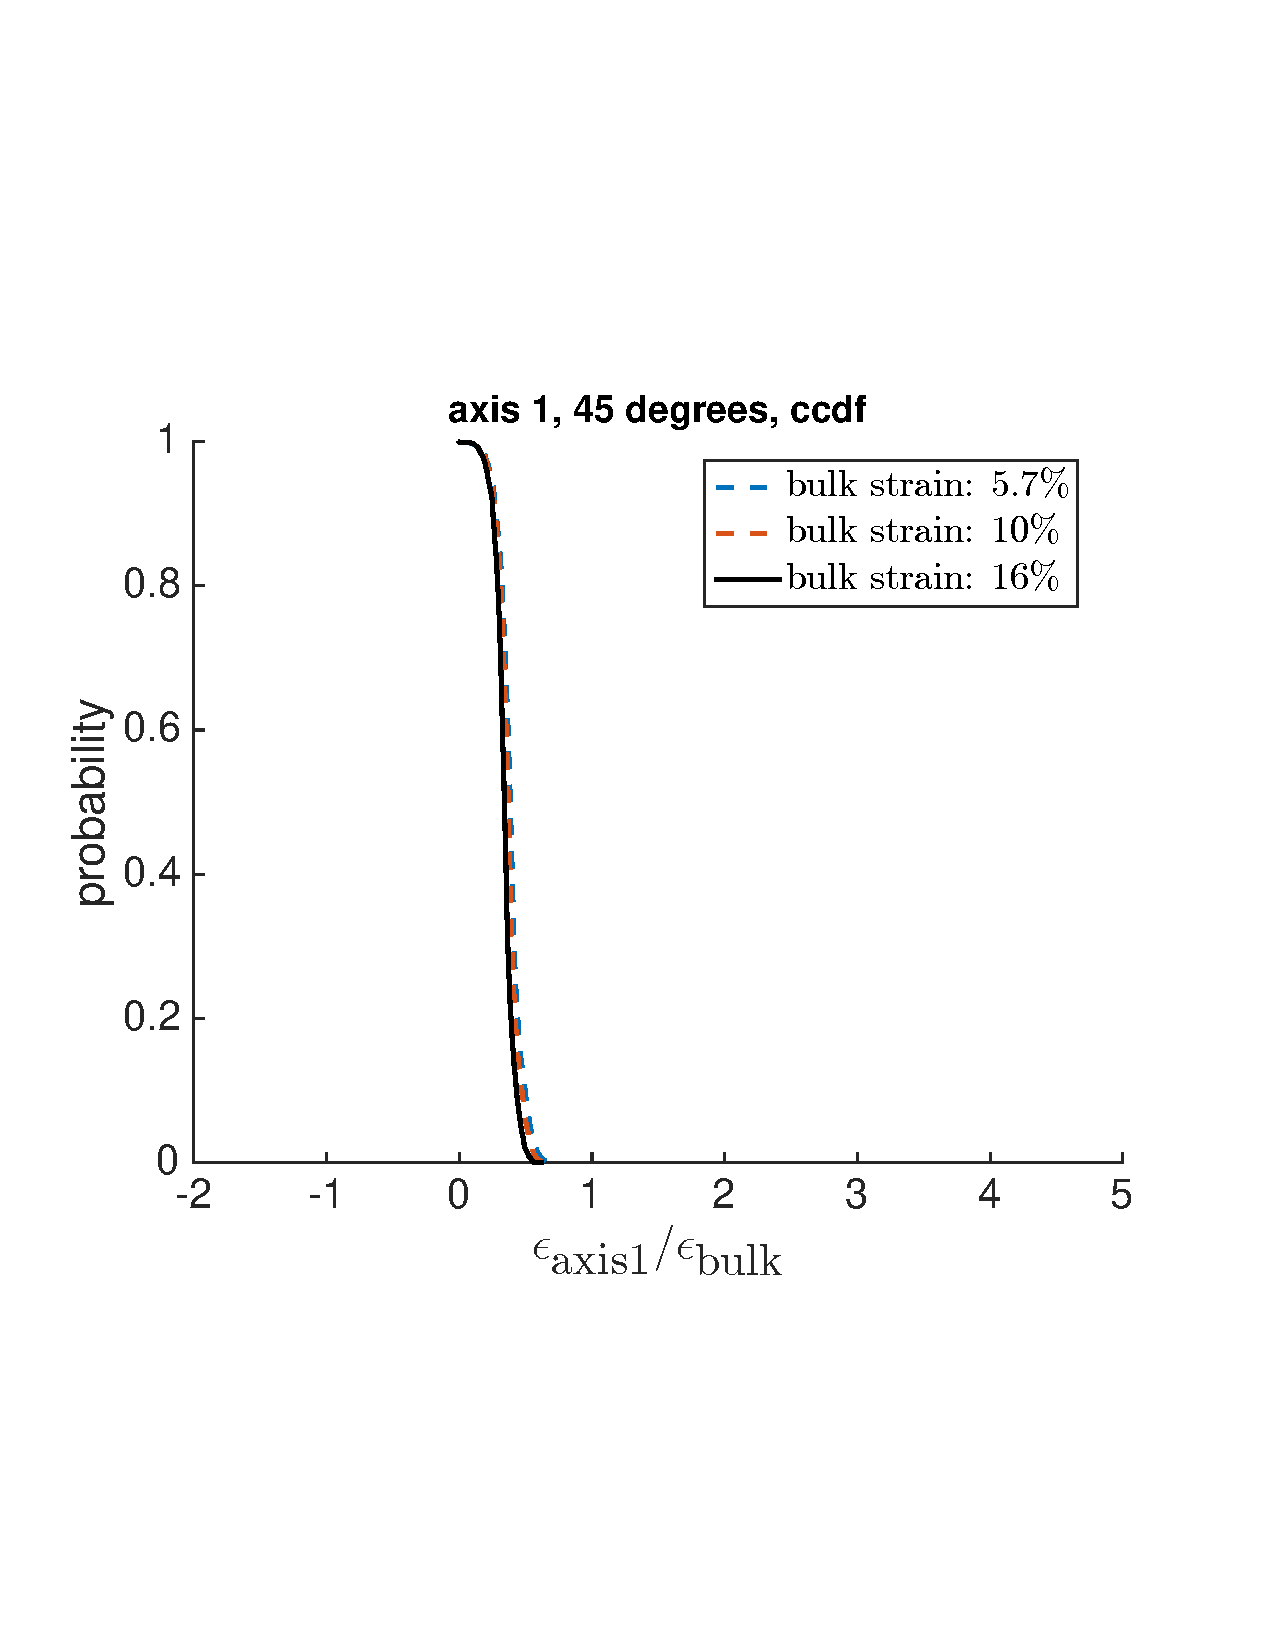
\includegraphics[height=4.5cm]{figure/rot45_FT50_strn11_128_1920_axial_ccdf_axis1_compare_stps.pdf} & 
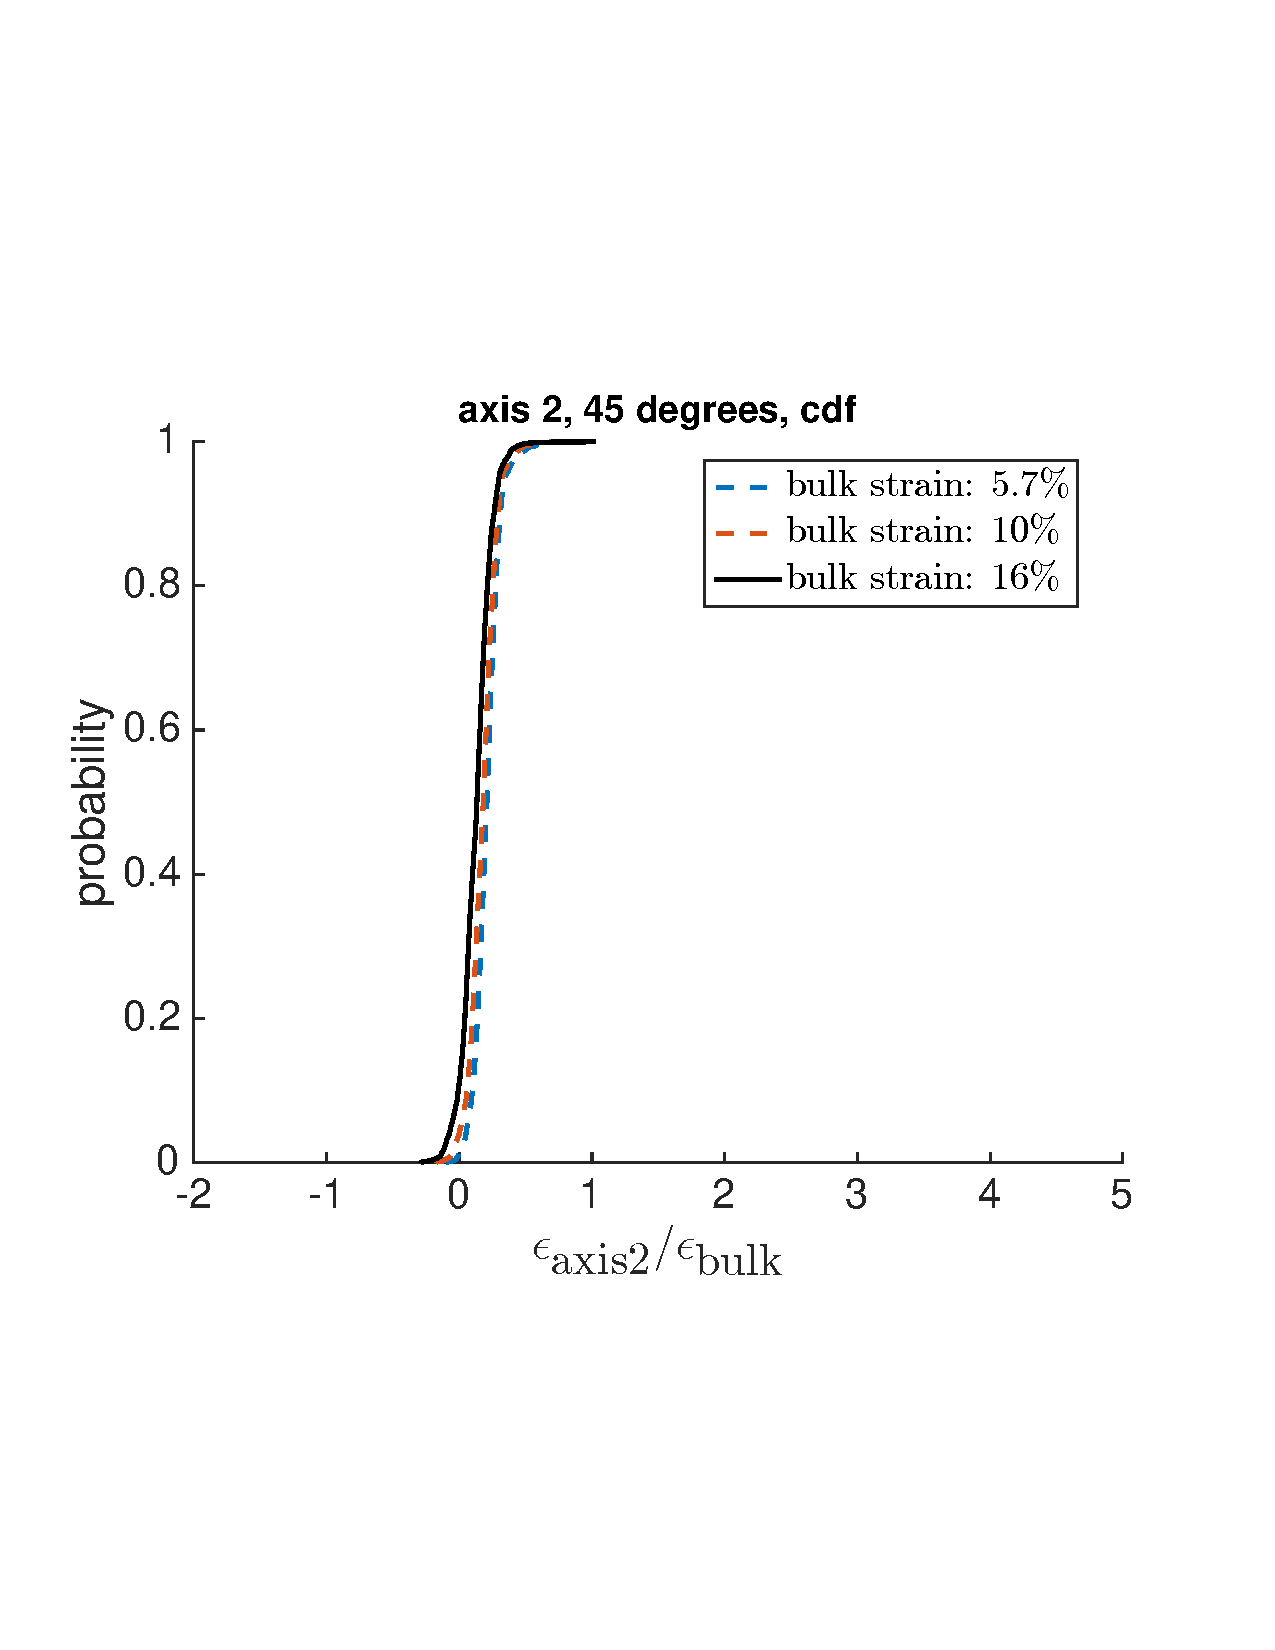
\includegraphics[height=4.5cm]{figure/rot45_FT50_strn22_128_1920_axial_cdf_axis1_compare_stps.pdf} & 
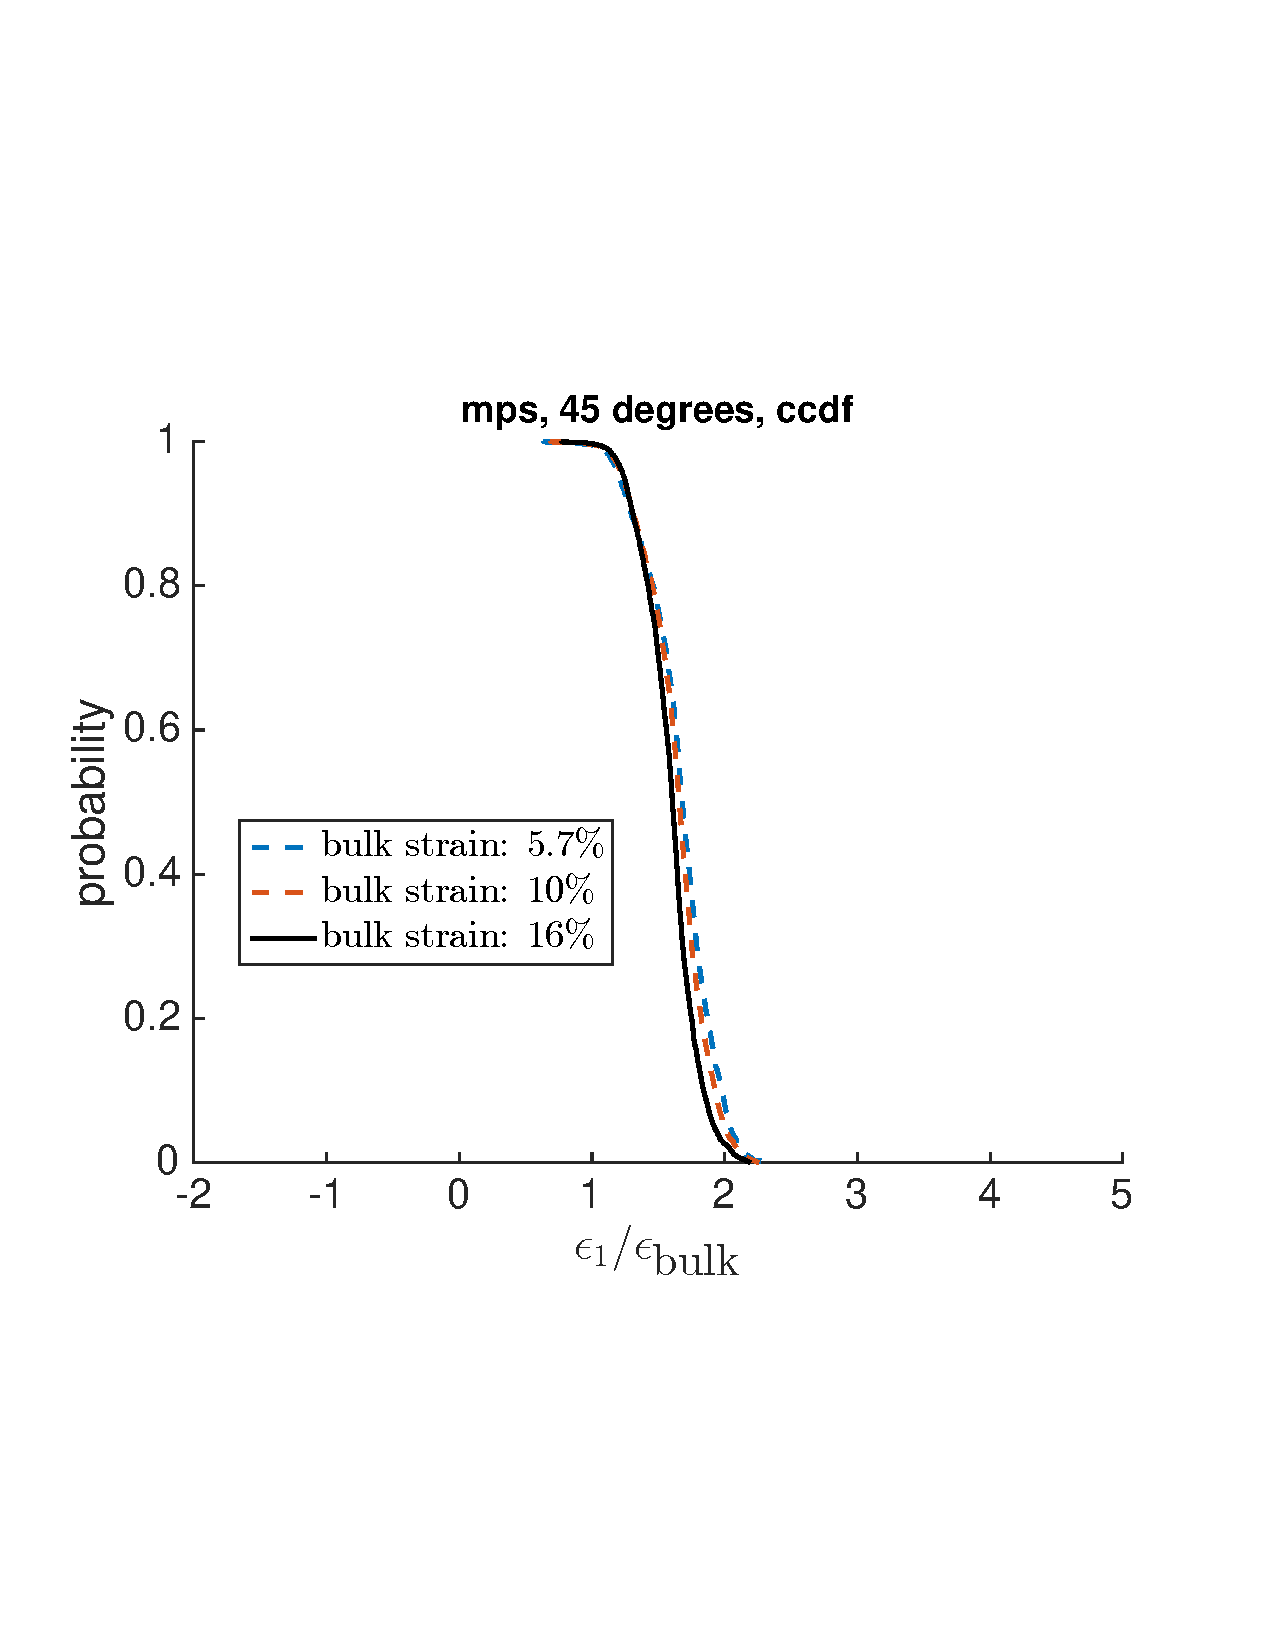
\includegraphics[height=4.5cm]{figure/rot45_FT50_strn11_128_1920_mps_ccdf_axis1_compare_stps.pdf} \\
(d) & (e) & (f) \\
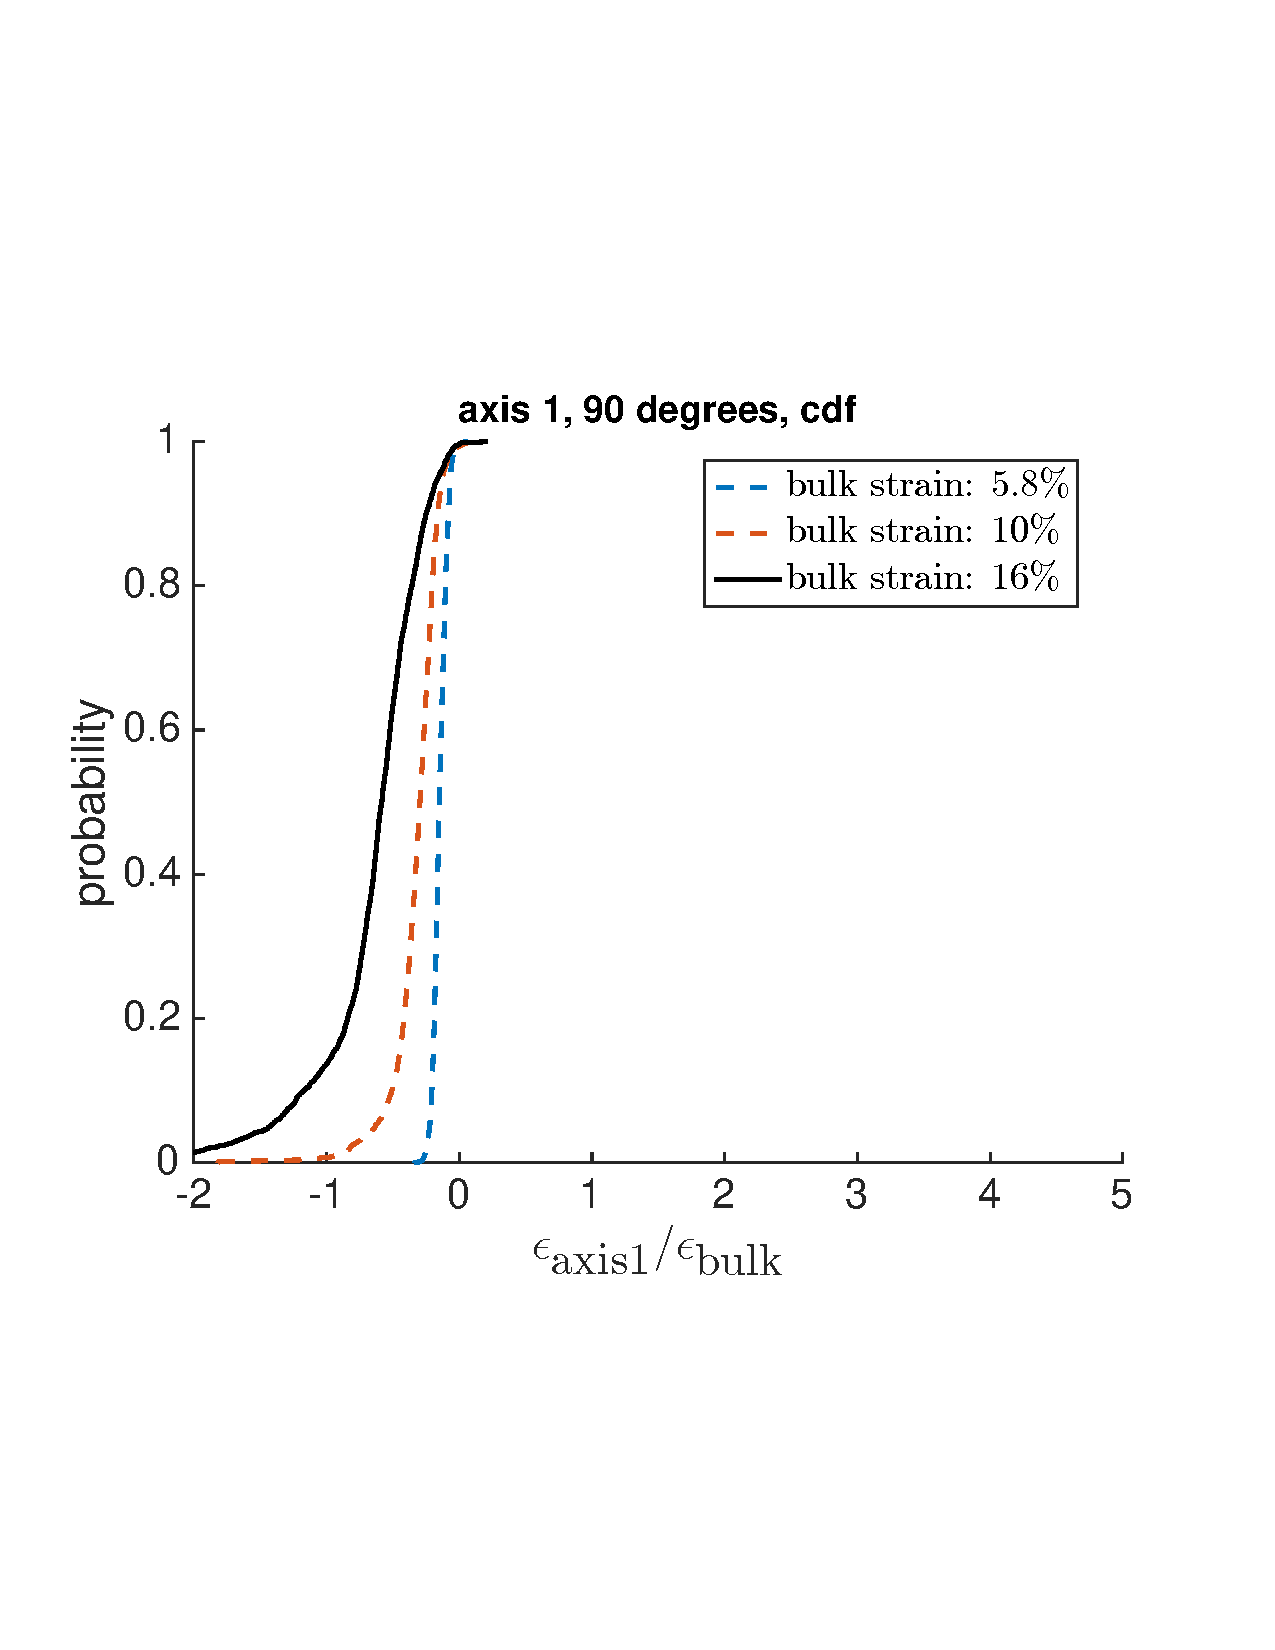
\includegraphics[height=4.5cm]{figure/rot90_FT50_strn11_128_1920_axial_cdf_axis1_compare_stps.pdf} & 
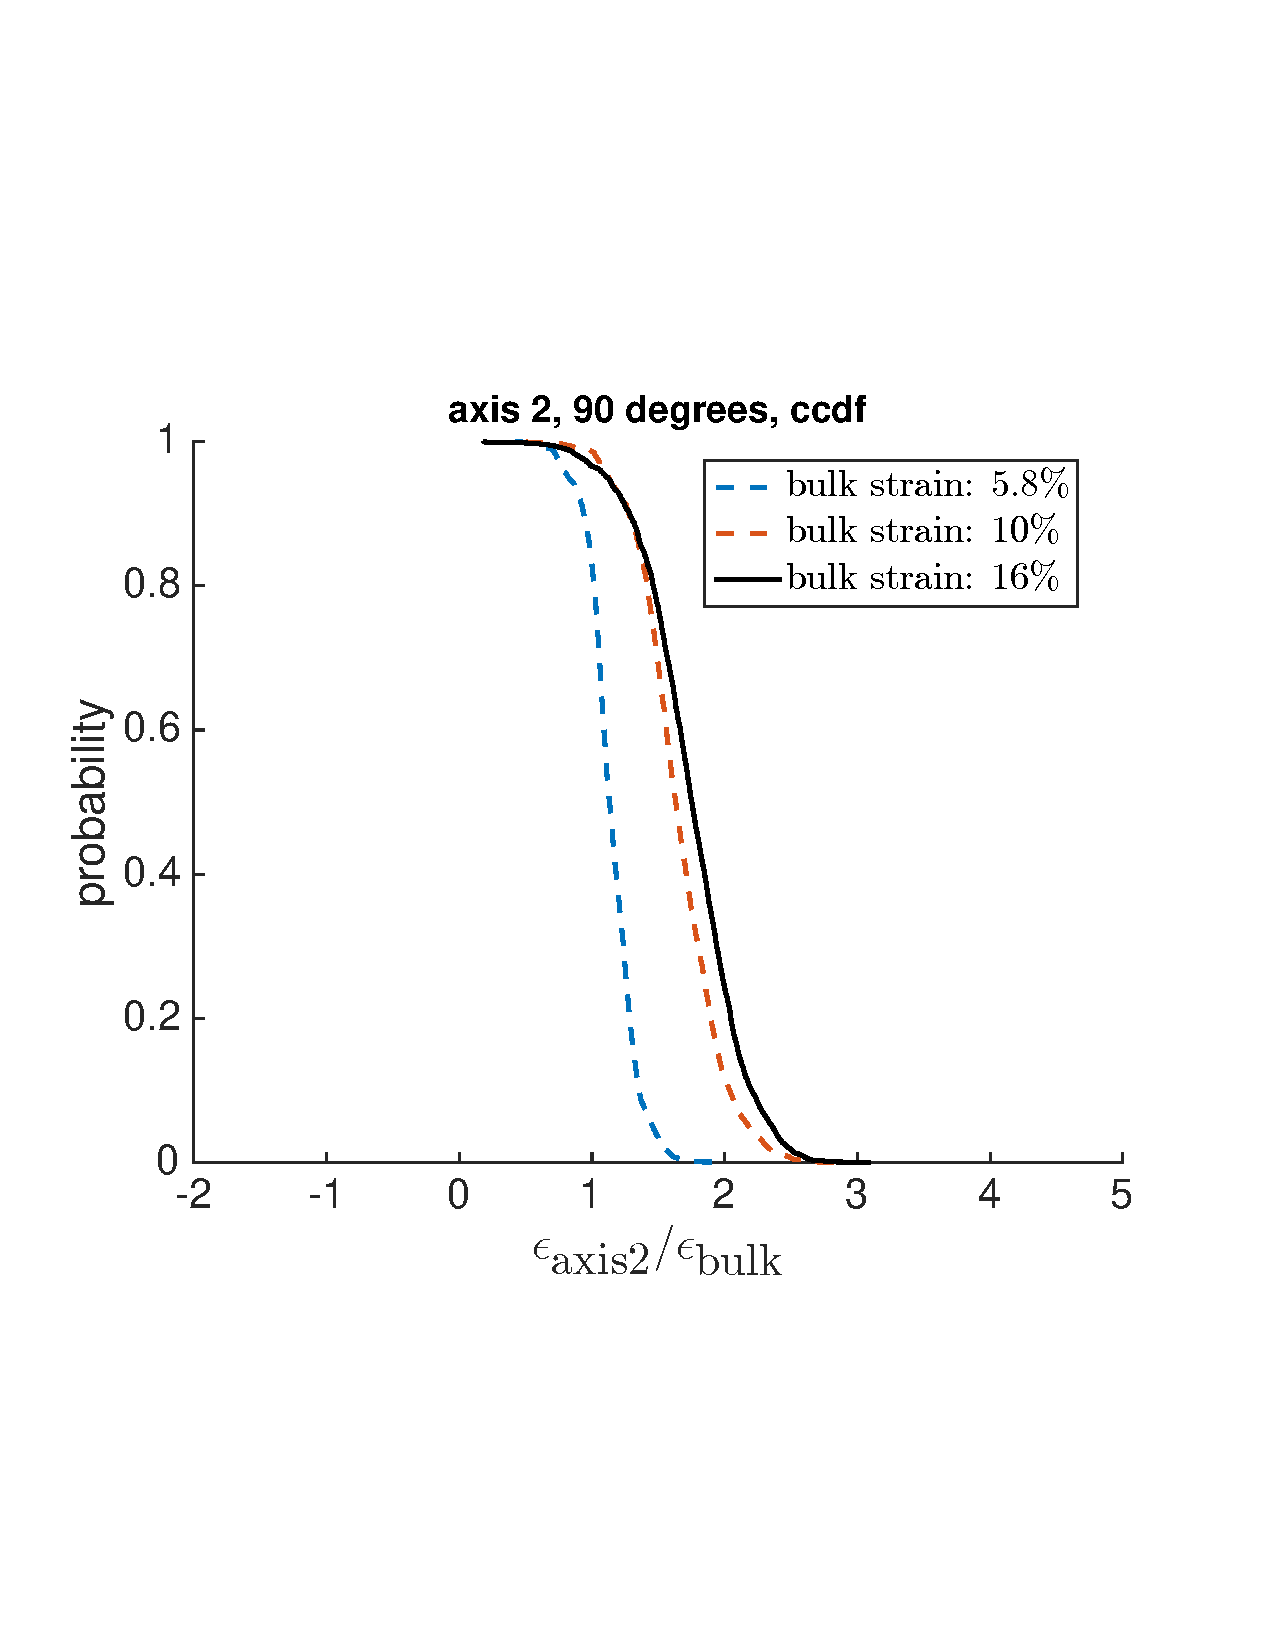
\includegraphics[height=4.5cm]{figure/rot90_FT50_strn22_ptdata_128_1920_axial_ccdf_axis1_compare_stps.pdf} & 
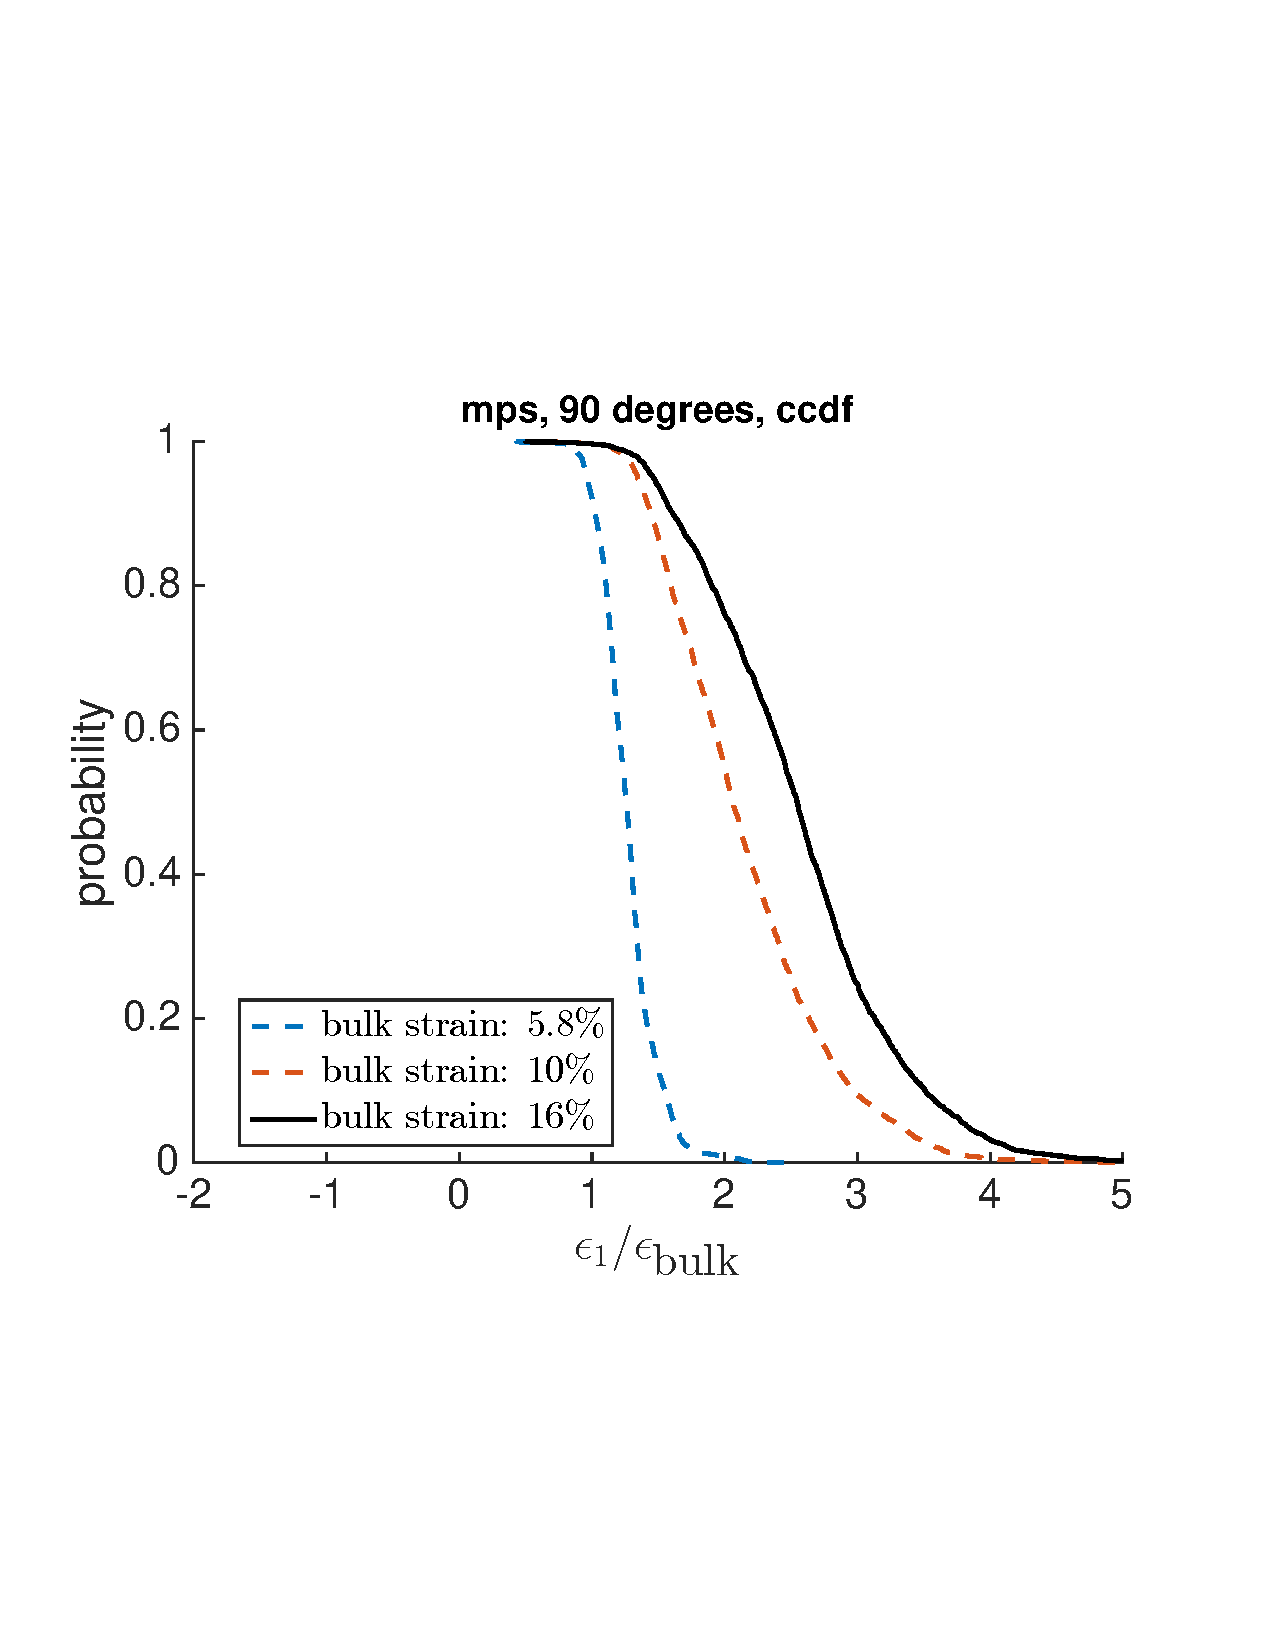
\includegraphics[height=4.5cm]{figure/rot90_FT50_strn11_128_1920_mps_ccdf_axis1_compare_stps.pdf} \\
(g) & (h) & (i) 
\end{array}
$
\end{center}
\caption{\label{fig:axial_mps_distr} Distributions of axial strain along axis 1 (left column), axial strain along axis 2 (middle column), and maximum principal strain (right column). The ccdf is plotted for tensile strains, while the cdf is plotted for compressive strains. Distributions for three bulk strains are shown in each plot.}
\end{figure}
%

As seen in Fig.\ \ref{fig:axial_mps_distr}, the strain distributions (axial and maximum principal strains) vary most significantly for the 90 degree loading case where  strains increase in magnitude with bulk strain in the gel. On the other hand, only small variations are seen in the strain distributions for the 0 and 45 degree loading cases. The local-strain amplification corresponding to the portion of the structure that experiences the largest 5$\%$ strain (0.05 on ordinate of distributions in Fig.\ \ref{fig:axial_mps_distr}) are plotted as a function of bulk strain in Fig.\ \ref{fig:axial_mps_amp}. The local-strain amplification measures how the neuron deforms when a load is applied to the surrounding gel, which can provide physiological insight into how nerves can be damaged when the surrounding tissue is being deformed.
%
\begin{figure}[ht]
\begin{center}
$
\begin{array}{ccc}
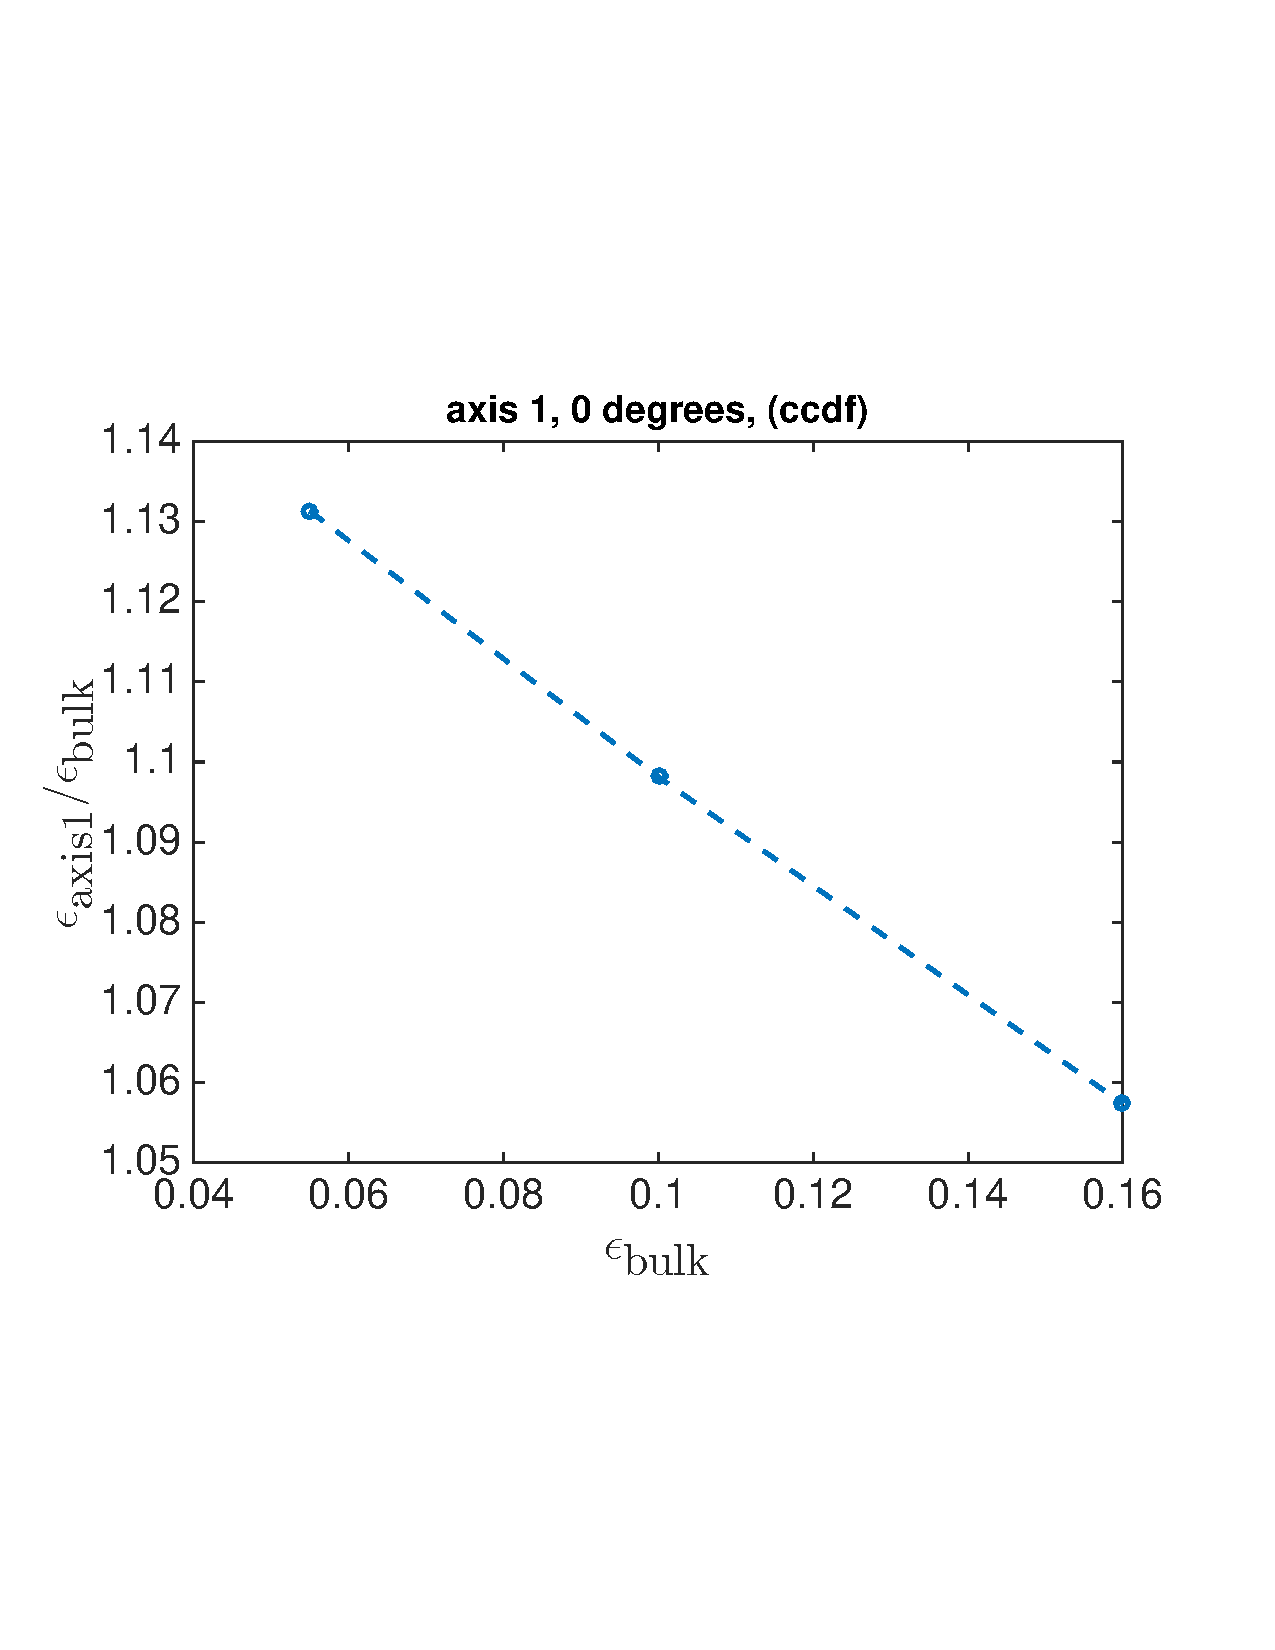
\includegraphics[height=4cm]{figure/rot0_FT50_strn11_128_1920_axial_ccdf_axis1_strn_amp.pdf} & 
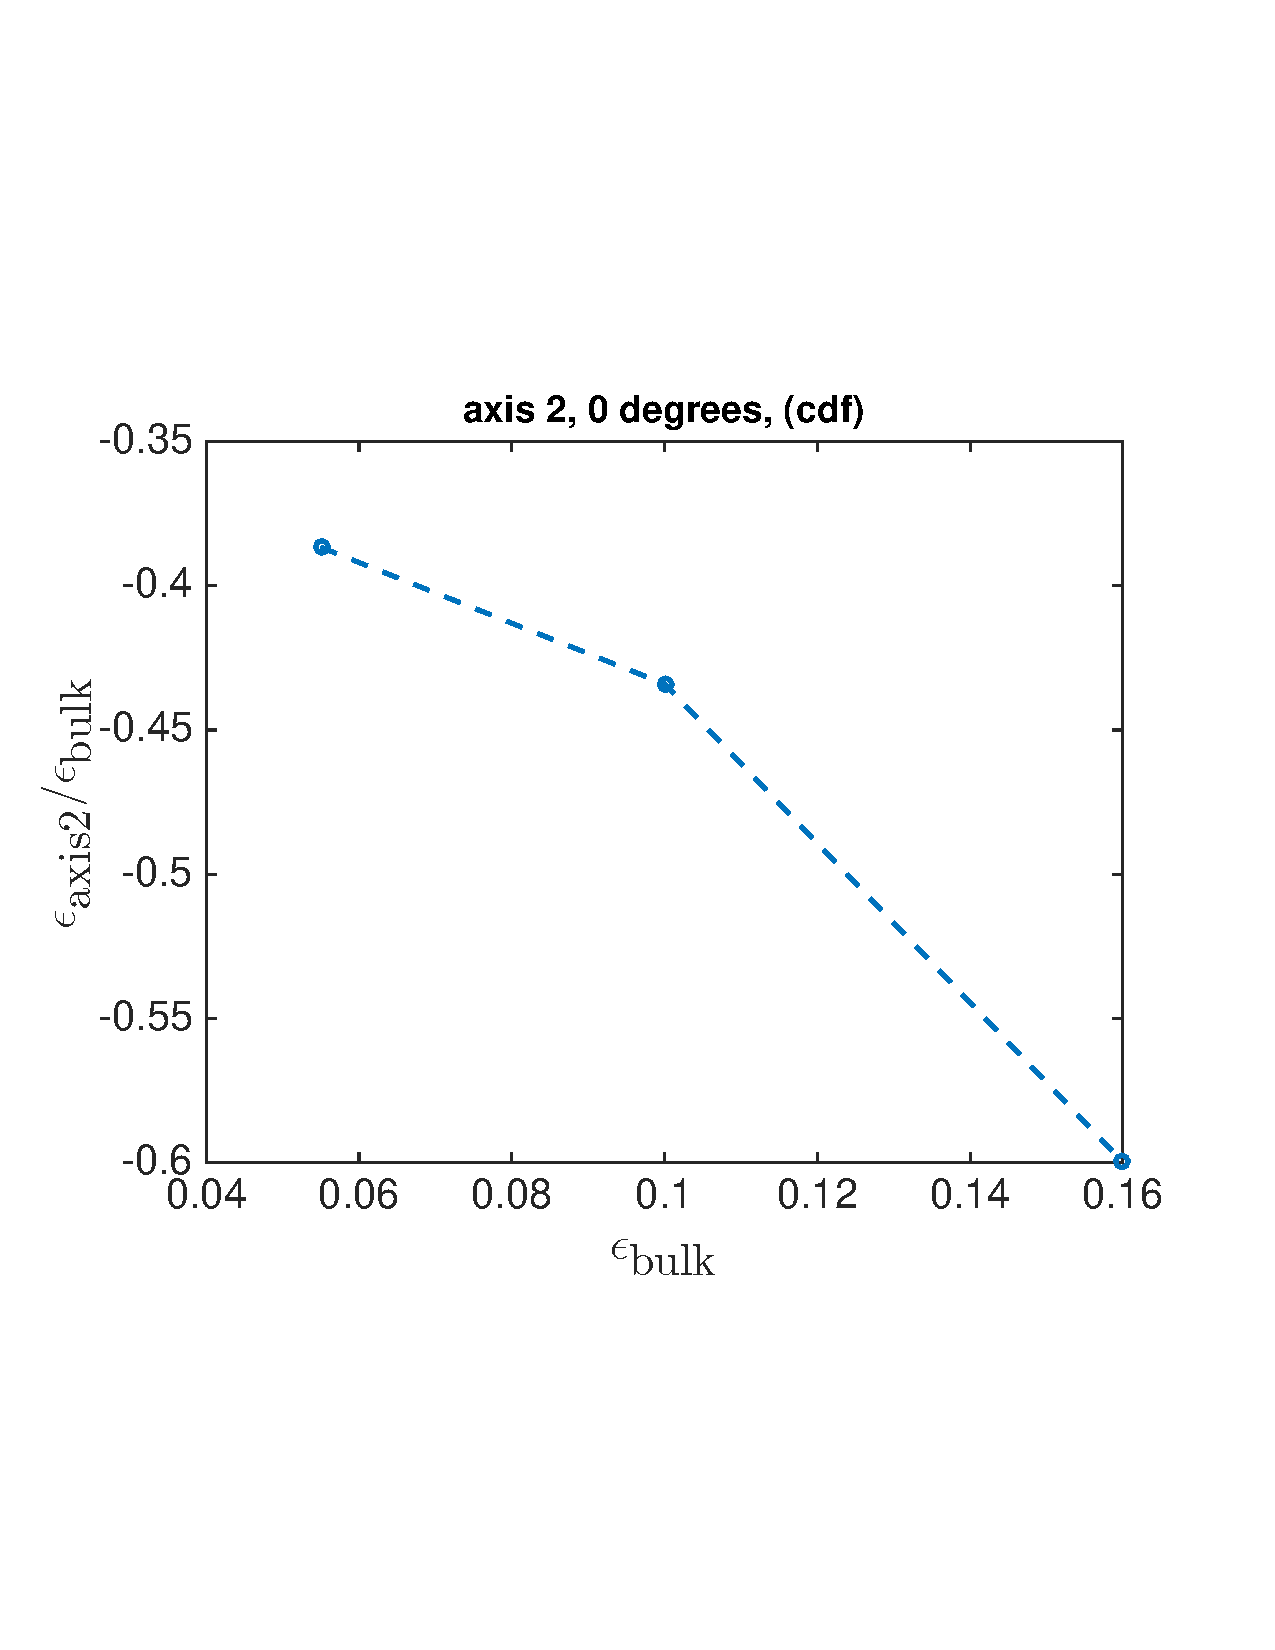
\includegraphics[height=4cm]{figure/rot0_FT50_strn22_128_1920_axial_cdf_axis1_strn_amp.pdf} & 
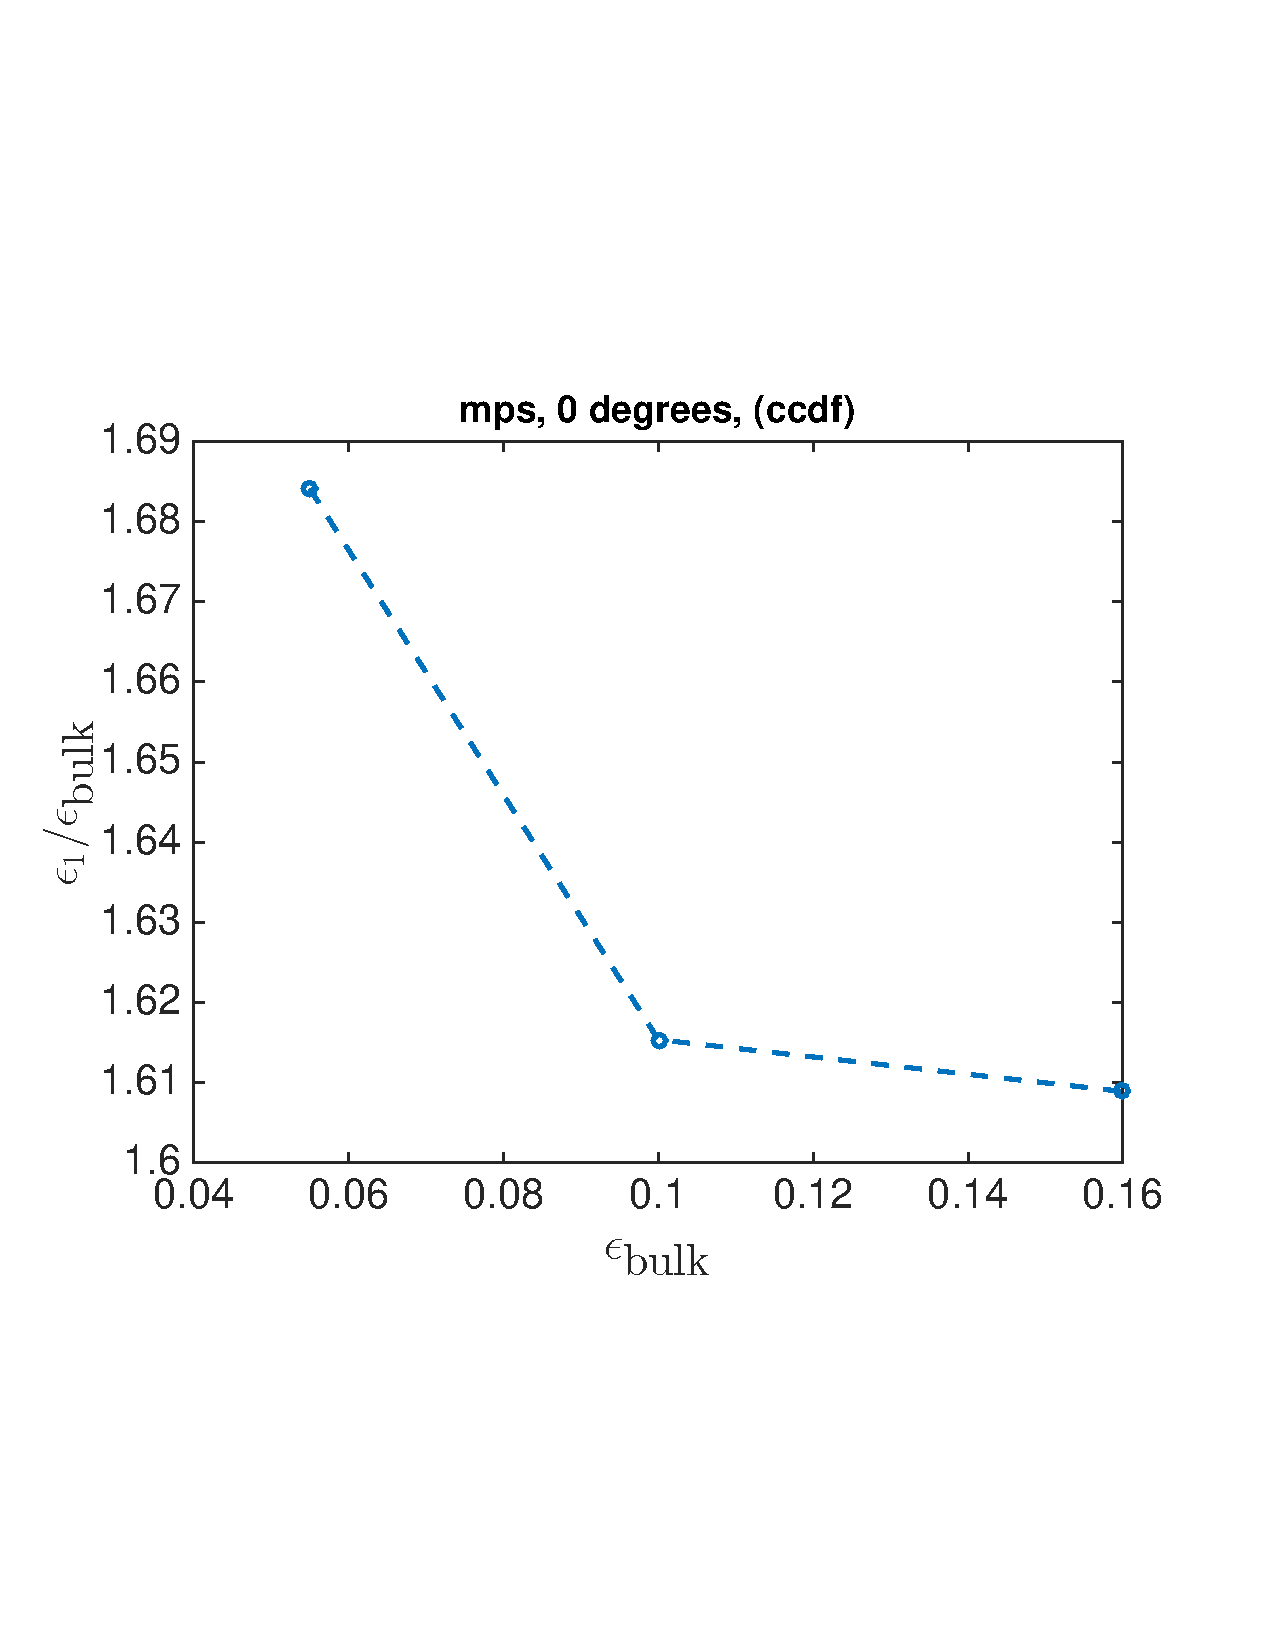
\includegraphics[height=4cm]{figure/rot0_FT50_strn11_128_1920_mps_ccdf_axis1_strn_amp.pdf} \\
(a) & (b) & (c) \\ 
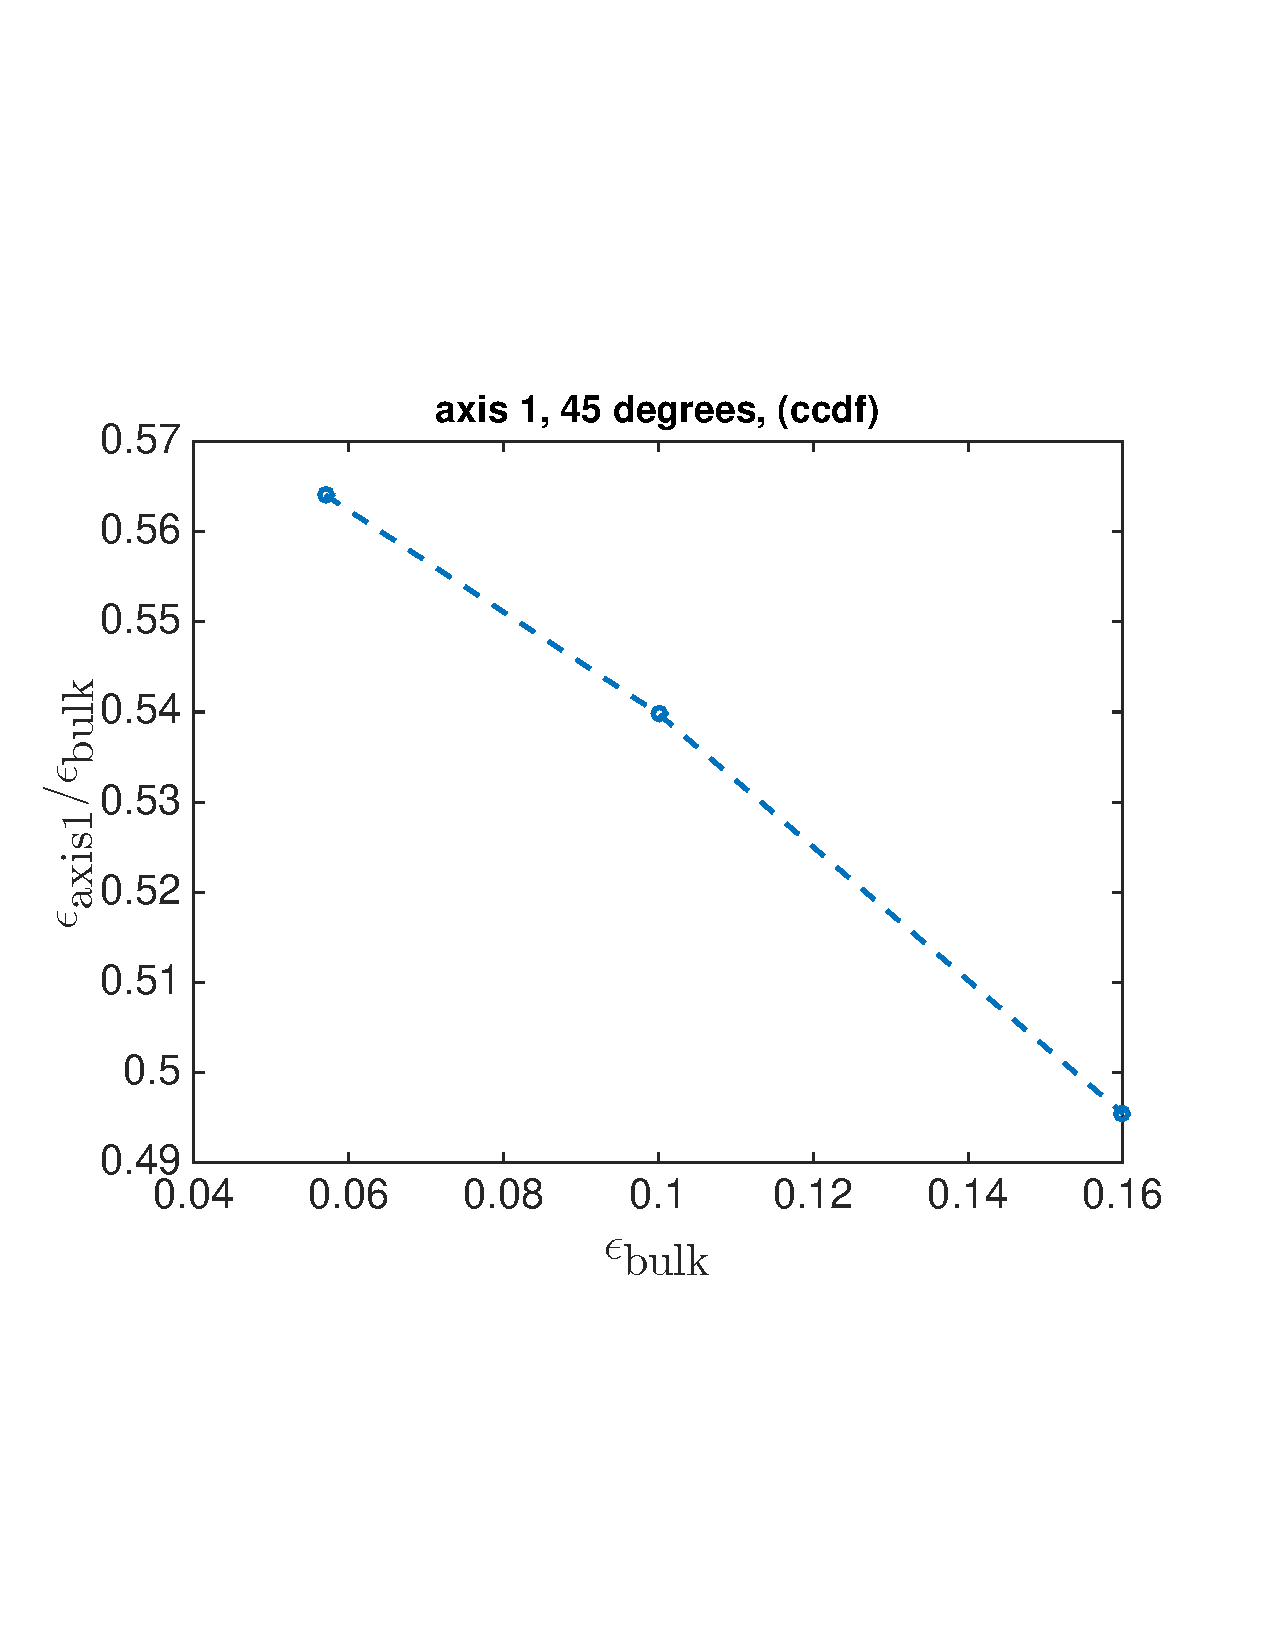
\includegraphics[height=4cm]{figure/rot45_FT50_strn11_128_1920_axial_ccdf_axis1_strn_amp.pdf} & 
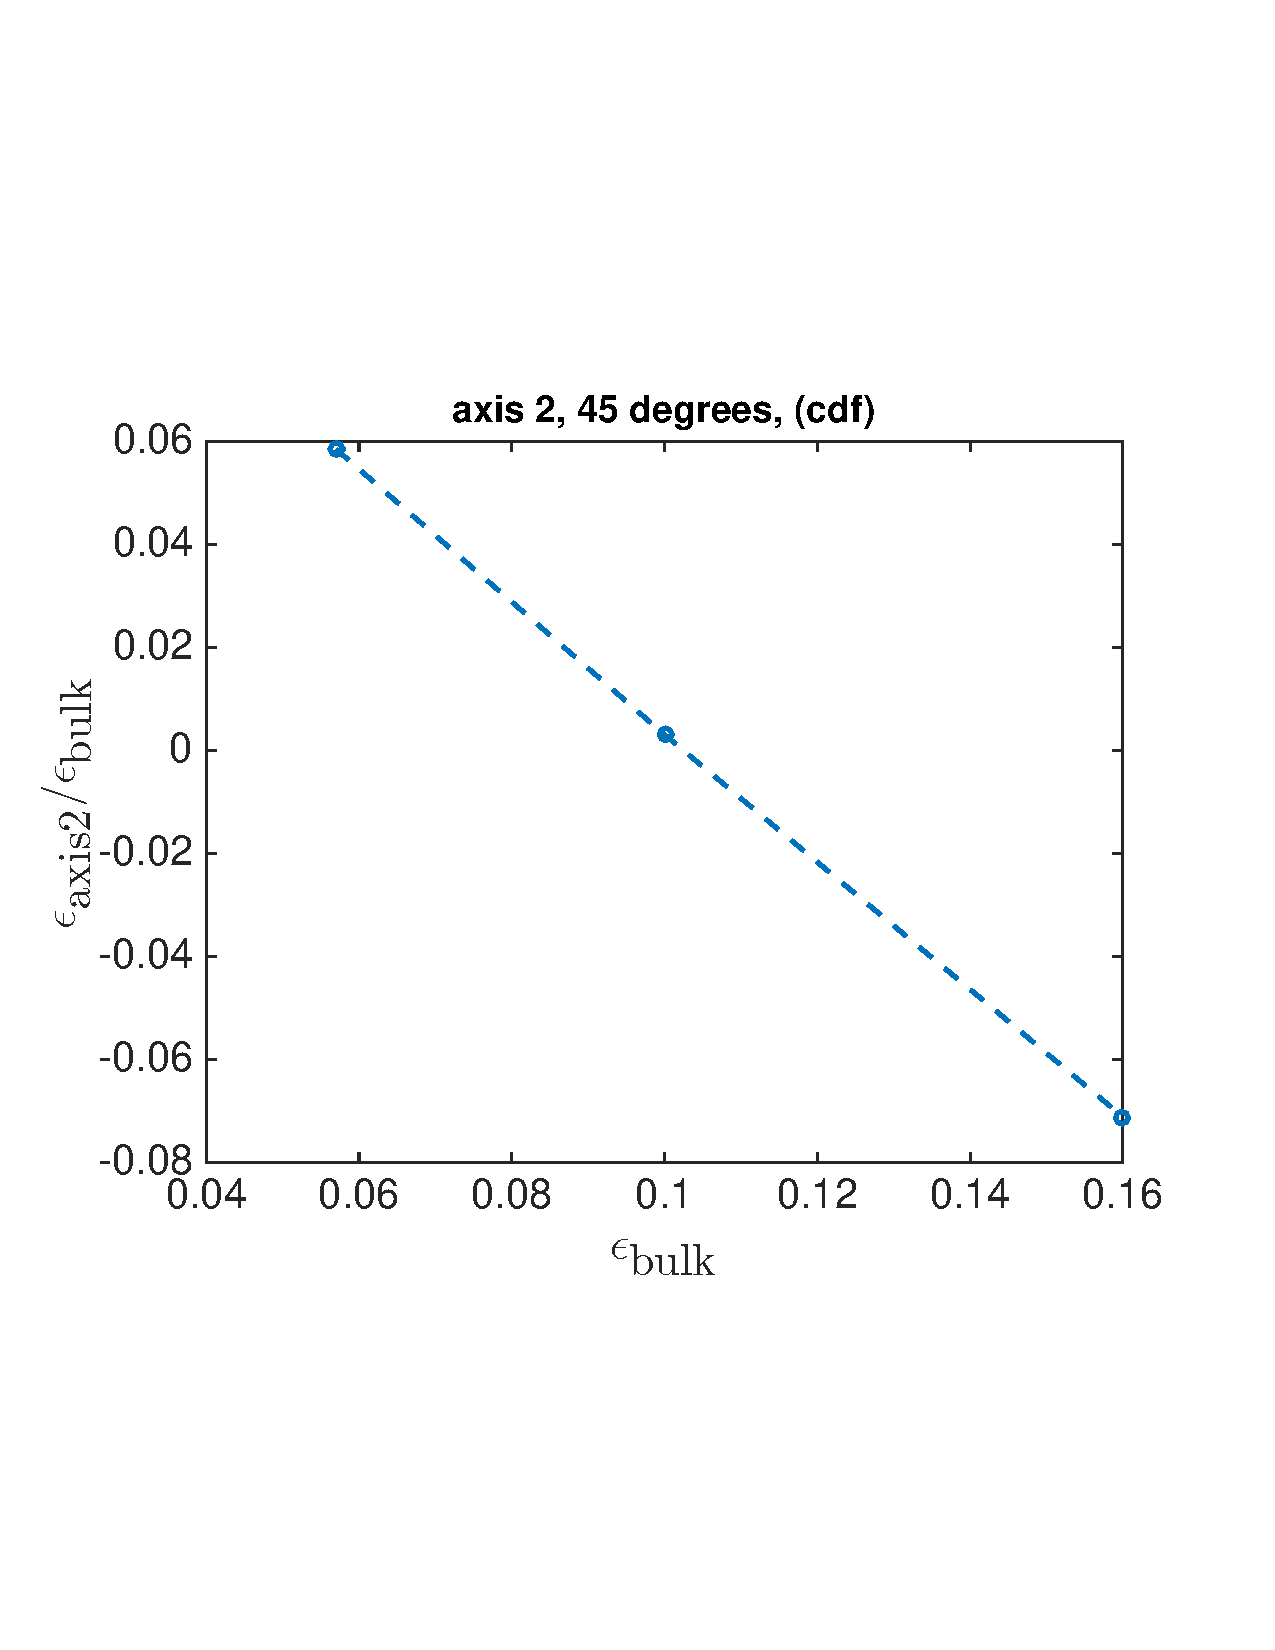
\includegraphics[height=4cm]{figure/rot45_FT50_strn22_128_1920_axial_cdf_axis1_strn_amp.pdf} & 
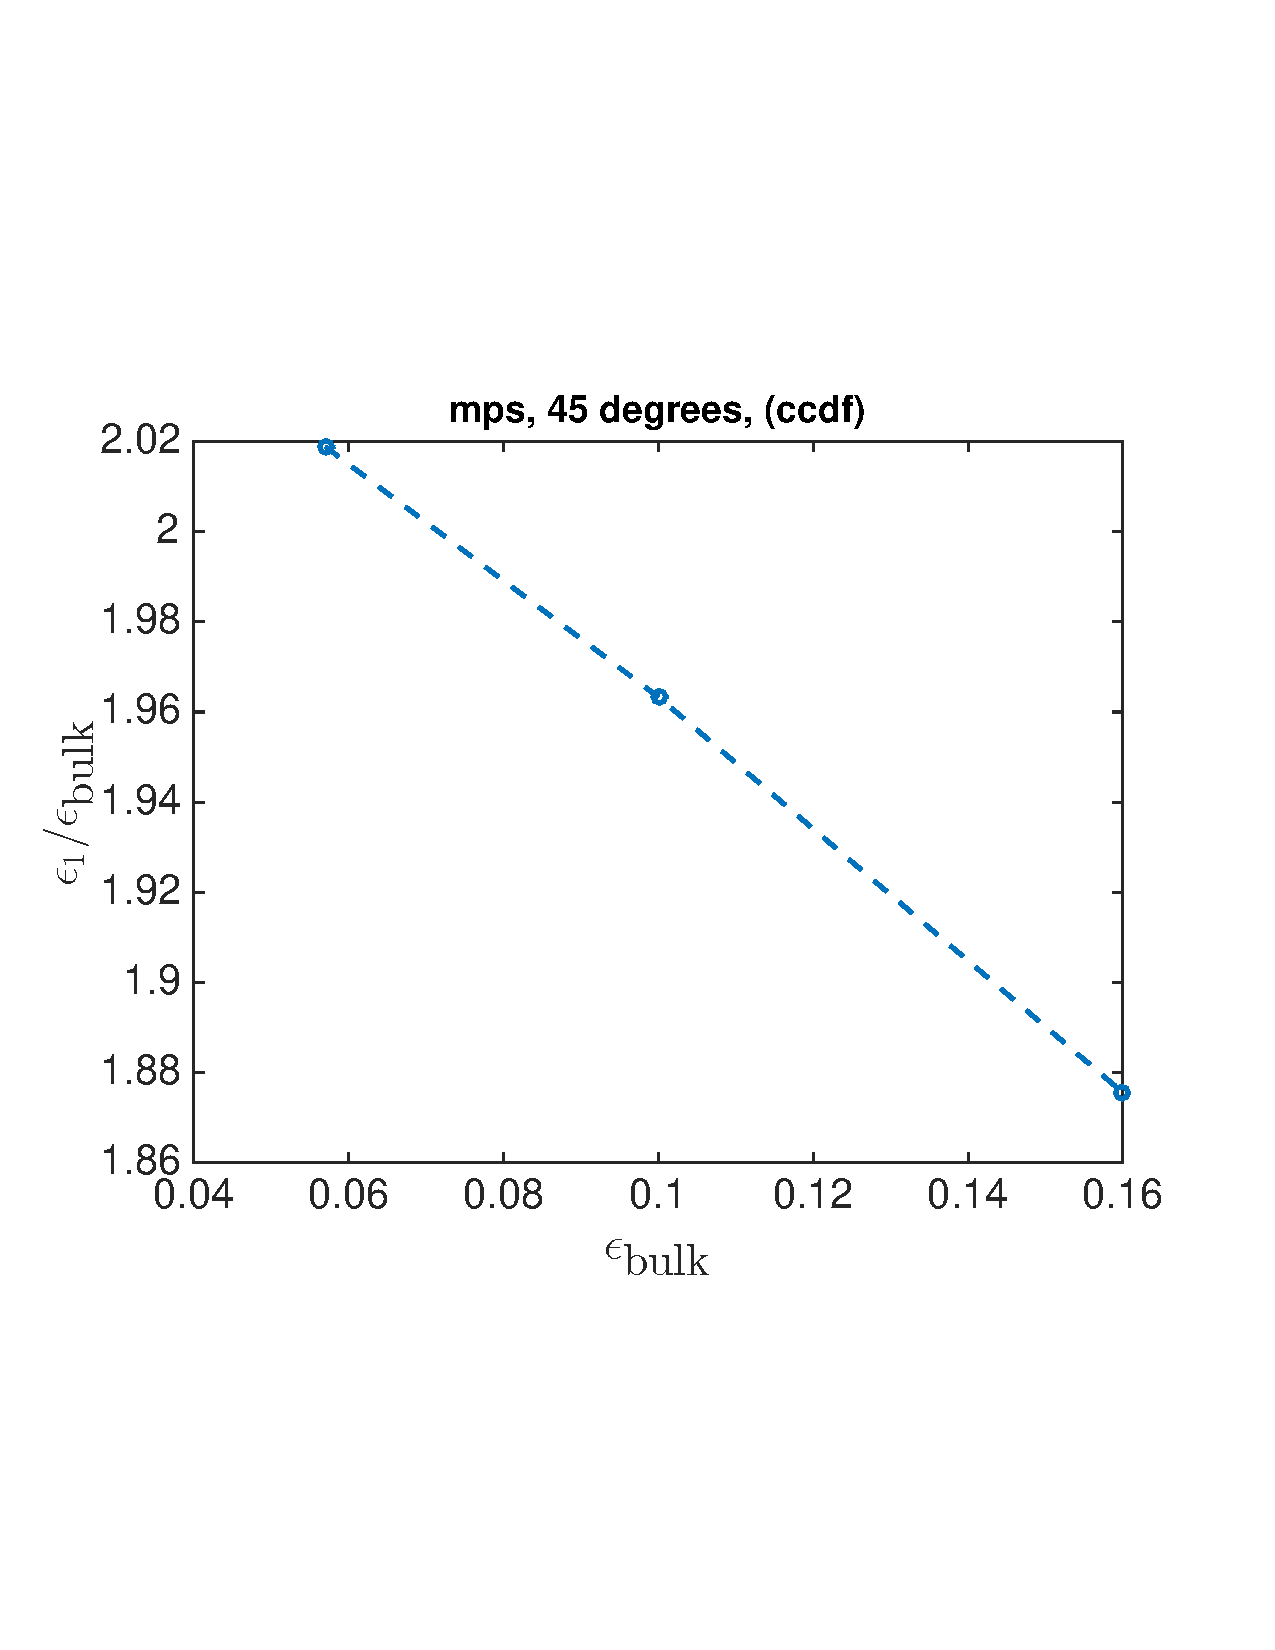
\includegraphics[height=4cm]{figure/rot45_FT50_strn11_128_1920_mps_ccdf_axis1_strn_amp.pdf} \\
(d) & (e) & (f) \\
\includegraphics[height=4cm]{figure/rot90_FT50_strn11_128_1920_axial_cdf_axis1_strn_amp.pdf} & 
\includegraphics[height=4cm]{figure/rot90_FT50_strn22_128_1920_axial_ccdf_axis1_strn_amp.pdf} & 
\includegraphics[height=4cm]{figure/rot90_FT50_strn11_128_1920_mps_ccdf_axis1_strn_amp.pdf} \\
(g) & (h) & (i) 
\end{array}
$
\end{center}
\caption{\label{fig:axial_mps_amp} Strain amplification corresponding to the portion of the neuron structure in Fig.\ \ref{fig:axial_schematic} that experiences the largest 5$\%$ strain (0.05 on ordinate of distributions in Fig.\ \ref{fig:axial_mps_distr}) as a function of bulk strain for different directions of loading.}
\end{figure}
%

To explain the trends seen in the local-strain amplification plots of Fig.\ \ref{fig:axial_mps_amp}, consider the following three major contributions when the a collagen gel surrounding the neuron structure in Fig.\ \ref{fig:axial_schematic}. Firstly, when the surrounding gel is deformed, the axial direction of embedded neuron structure becomes increasingly aligned with the direction of loading. Since the neuron structure is significantly stiffer in the axial direction, the relative stiffness of the neuron structure increases. Secondly, when the surrounding gel is deformed, the stiffness of the gel increases (see stress-strain curve in Fig.\ \ref{fig:fiber_param}(a)). The stiffening of the surrounding gel causes the neuron to become relatively softer. Thirdly, when the surrounding gel is deformed, the Poisson ratio of the gel increases (see Poisson ratio curve in Fig.\ \ref{fig:fiber_param2}(a)). The increase in the Poisson ratio results in an increasing lateral compressive strain when the gel is deformed. Note that the first and second contributions give rise to opposite effects, while the third contribution is related to deformations in the lateral directions of the applied load.

In the case of 0 degree loading, the decreasing local-strain amplification along axis 1 (Fig.\ \ref{fig:axial_mps_amp}(a)) indicates that the neuron structure becomes relatively stiffer than the gel as the gel is deformed. Physically, this suggests that the contribution from the alignment of the neuron structure is larger than the contribution from the gel becoming stiffer. The increasing compressive strain along axis 2 (Fig.\ \ref{fig:axial_mps_amp}(b)) is consistent with the fact that the Poisson ratio of the gel increases as the gel is deformed (third contribution). A similar trend to 0 degree loading is seen in axis 1 for the 45 degree loading case (Fig.\ \ref{fig:axial_mps_amp}(d)) where the first contribution from the alignment of the neuron structure is larger than the second contribution from the stiffening of the gel. The difference in magnitude of the amplification is due to the initial alignment of the neuron structure relative to the applied load. The trend is also similar to 0 degree loading in axis 2 for the 45 degree loading case (Fig.\ \ref{fig:axial_mps_amp}(e)), with the exception that axis 2 experiences some tensile strain at smaller bulk strains before the lateral compressive strains that arise from the Poisson ratio effect become large.

In the case of 90 degree loading, the strains experienced along axes 1 and 2 are switched relative to the 0 degree loading case because the load directions are orthogonal. Interestingly, contrary to the 0 degree loading case, the local-strain amplification along axis 2 (the tensile strain scenario) increases as deformation on the gel increases indicating that the neuron becomes relatively softer than the surrounding gel. Physically, this indicates that the second contribution of gel stiffening is much larger than that of the first contribution of the neuron structure aligning with the load direction. On the other hand, the amplification in the strains along axis 1 (the compressive strain scenario) is similar to that of the 0 degree loading case where the amplification of the compressive strain increases with gel deformation. \textcolor{red}{Additionally, softening of neuron structure in axis 2 gives rise to larger local compressive strain?}.

\subsection{Fiber Alignment in Collagen Gel}

%
\begin{figure}[ht]
\begin{center}
$
\begin{array}{ccc}
\includegraphics[height=4cm]{figure/rot0_FT50_128_1920_histo_gel_5.pdf} & 
\includegraphics[height=4cm]{figure/rot45_FT50_128_1920_histo_gel_8.pdf} &
\includegraphics[height=4cm]{figure/rot90_FT_dspBC50_a30_128_1920_histo_gel_27.pdf} \\
(a) & (b) & (c) \\ 
\includegraphics[height=4cm]{figure/rot0_FT50_128_1920_histo_gel_20.pdf} &
\includegraphics[height=4cm]{figure/rot45_FT50_128_1920_histo_gel_20.pdf} &
\includegraphics[height=4cm]{figure/rot90_FT_dspBC50_a30_128_1920_histo_gel_47.pdf} \\
(d) & (e) & (f)
\end{array}
$
\end{center}
\caption{\label{fig:gel_P2} Distribution of $P_2$ in collagen gel for applied loads at 0 degrees (left column), 45 degrees (middle column), and 90 degrees (right column). The distributions for 10$\%$ (top row) and 16$\%$ (bottom row) bulk strain are shown. $P_2$ is calculated relative to the [1,0,0] axis, i.e., the axis along the direction of 0 degrees applied load.}
\end{figure}
%

%
\begin{figure}[ht]
\begin{center}
$
\begin{array}{c}
\includegraphics[height=6cm]{figure/avgP2.pdf} 
\end{array}
$
\end{center}
\caption{\label{fig:avg_P2} Average of $P_2$ in the gel for applied loads at 0, 45, and 90 degrees. $P_2$ is calculated relative to the [1,0,0] axis, i.e., the axis along the direction of 0 degrees applied load.}
\end{figure}
%
%%%%%%%%%%%%%%%%%%%%%%%%%%%%%%%%%%%%%%%%%%%%%%%%%%%%%%%%%%%%%%%%%%%%%%
\section{Conclusion}

%%%%%%%%%%%%%%%%%%%%%%%%%%%%%%%%%%%%%%%%%%%%%%%%%%%%%%%%%%%%%%%%%%%%%%
\begin{acknowledgment}

\end{acknowledgment}

%%%%%%%%%%%%%%%%%%%%%%%%%%%%%%%%%%%%%%%%%%%%%%%%%%%%%%%%%%%%%%%%%%%%%%
% The bibliography is stored in an external database file
% in the BibTeX format (file_name.bib).  The bibliography is
% created by the following command and it will appear in this
% position in the document. You may, of course, create your
% own bibliography by using thebibliography environment as in
%
% \begin{thebibliography}{12}
% ...
% \bibitem{itemreference} D. E. Knudsen.
% {\em 1966 World Bnus Almanac.}
% {Permafrost Press, Novosibirsk.}
% ...
% \end{thebibliography}
\newpage
% Here's where you specify the bibliography style file.
% The full file name for the bibliography style file 
% used for an ASME paper is asmems4.bst.
\bibliographystyle{asmems4}

% Here's where you specify the bibliography database file.
% The full file name of the bibliography database for this
% article is asme2e.bib. The name for your database is up
% to you.
\bibliography{references}


\end{document}
